\chapter{Effects of placental structure on placental efficiency} \label{sec:nutrient-uptake}
    % \todoitemtwo{Simplify discussion of results}
    % \todoitemthree{Visualise artery width solutions}
    
    One of the main functions of the placenta is to deliver oxygen and nutrients to the developing fetus, with impaired delivery being characteristic of diseases such as fetal growth restriction (FGR) or pre-eclampsia (PE) \cite{jensenBloodFlowTransport2019,burtonRheologicalPhysiologicalConsequences2009,burtonPathophysiologyPlacentalderivedFetal2018,dellschaftHaemodynamicsHumanPlacenta2020,serovOptimalVilliDensity2015}. In this chapter, we will use the blood flow and oxygen transport models from Chapter \ref{sec:modelling} and numerical methods from Chapter \ref{sec:numerical-methods} to study changes in the flow and oxygen concentration fields due to structural variations in the placenta. We will primarily investigate changes to these fields via seven different proxy quantities that capture the main features of the flow and oxygen transport fields.
    
    In Chapter \ref{sec:introduction}, we commented on the difficulties in determining the number of vessels in the placenta. Several papers in the literature include measurements or estimates of the number of spiral arteries in the placenta, of which there are thought to be between $30$ and $150$ \cite{benirschkePathologyHumanPlacenta2012,chernyavskyMathematicalModelIntervillous2010,kaufmannPlacentalVascularizationBlood1988}. Information on the number of veins is scarcer: according to \citeauthor{chernyavskyMathematicalModelIntervillous2010} \cite{chernyavskyMathematicalModelIntervillous2010}, the placenta may contain between $50$ and $200$ veins in total. The wide range of numbers of arteries and veins suggests either a high variation in individual placentas or a lack of understanding. It is therefore important to understand how the numbers of arteries and veins, and the ratio between them, affects the placenta.
    
    As well as the number of vessels (where we refer to `vessels' as arteries and veins collectively), there is also uncertainty in their position. Most mathematical studies on vessels thus far have been limited to, for example, symmetric placement of basal plate veins \cite{chernyavskyMathematicalModelIntervillous2010}, or to study of the shape of arteries \cite{burtonRheologicalPhysiologicalConsequences2009,rothDynamicModelingUteroplacental2017}. \citeauthor{meklerImpactTissuePorosity2022} \cite{meklerImpactTissuePorosity2022} in \citeyear{meklerImpactTissuePorosity2022} took this a step further, investigating the effects of the number and asymmetric placement of basal plate veins; they found that higher numbers of veins placed symmetrically overall reduced oxygen concentration throughout the domain, which is likely related to the short-circuiting behaviour originally reported by \citeauthor{chernyavskyMathematicalModelIntervillous2010} \cite{chernyavskyMathematicalModelIntervillous2010}, where flow exits through veins soon after entering the placenta. We expand upon the work of \citeauthor{meklerImpactTissuePorosity2022} \cite{meklerImpactTissuePorosity2022} in \S\ref{sec:nutrient-uptake:variation-of-vessels} by considering variations in the number and placement of arteries and veins across a 2D slice of a placenta.

    In addition to the number and position of vessels, there are of course many other structural changes that have an impact on placental function. An example of this is the diameter of the spiral arteries, which is thought to play a role in diseased placentas. In healthy placentas, blood enters through a narrow artery of approximately \qty{0.5}{\milli\metre} that widens to \qtyrange{2}{3}{\milli\metre}, allowing upstream flow at approximately \qty{1}{\metre\per\second} to slow to approximately \qty{0.1}{\metre\per\second}; however in diseased cases, the failure to widen can result in flow at \qty{1}{\metre\per\second} to directly enter the placenta, causing damage to the villous tree material \cite{burtonRheologicalPhysiologicalConsequences2009}. 

    Another example of an impactful structural change is the density of the villous tree structure, which has been investigated mathematically. \citeauthor{serovOptimalVilliDensity2015} \cite{serovOptimalVilliDensity2015} used a stream-tube model of the villi to find an optimal villous tree density; in order to maximise oxygen uptake, they found a careful balance was required between the effects of reduced flow rates but increased uptake area from dense villous tree structure, and the effects of fast flow with a reduced uptake area from a coarse villous tree structure.

    Therefore, in addition to studying variations in the number and placement of vessels in \S\ref{sec:nutrient-uptake:variation-of-vessels}, we will also consider variations of seven other parameters in \S\ref{sec:nutrient-uptake:variation-of-other-parameters}: artery width, vein width, septal wall heights, oxygen diffusivity, oxygen uptake rate, permeability of the villous tree, and inlet blood speed.
    
    Firstly, in \S\ref{sec:nutrient-uptake:measures-of-efficiency}, we will define seven quantities to be used as a proxy for measuring placental efficiency. Secondly, in \S\ref{sec:nutrient-uptake:variation-of-vessels}, we will study how the number and positions of vessels affect placental efficiency; in particular, we will relax the assumption that arteries and veins are placed symmetrically in each placentone in specific positions. Thirdly, in \S\ref{sec:nutrient-uptake:variation-of-other-parameters}, we will study the dependence of placental efficiency due to changes in seven other parameters described above. Finally, we will conclude in \S\ref{sec:nutrient-uptake:summary} with an overview of the results and remarks on the physical consequences.
    
    \section{Measures of placental efficiency} \label{sec:nutrient-uptake:measures-of-efficiency}
        To investigate the effects of changes to placental structure and flow parameters on placental function, we introduce seven measures of placental efficiency. Each of these measures gives a single scalar value that characterises the flow and oxygen concentration fields; we use these measures on an ensemble of simulations to infer, for example, how the number of arteries may affect the amount of oxygen uptaken by the villous tree, or how the permeability of the villous tree affects the amount of slow flow in the placenta.
        
        The first gives a measure of blood flow speed by taking the integral average of the velocity magnitude over a given domain $\Omega$:
        \begin{equation}
            \bar{v}(\Omega) := \frac{1}{|\Omega|} \int_{\Omega} |\vec{u}| \diff \vec{x},
            \label{eq:eff-v}
        \end{equation}
        where $\vec{u}$ is the velocity of the blood flow, and $|\Omega| := \int_\Omega \diff \vec{x}$. The second measures the fraction of `slow flow' in the domain, i.e., the area fraction in which the flow speed is below a threshold, $V~\unit{\metre\per\second}$:
        \begin{equation}
            v_\text{slow}(V) := \frac{1}{|\Omega|} \int_\Omega \mathds{1}(|\vec{u}| < V) \diff \vec{x},
            \label{eq:eff-v-slow}
        \end{equation}
        where $\mathds{1}(|\vec{u}| < V)$ denotes the indicator function\footnote{The indicator function is defined at a point as $\mathds{1}(|\vec{u}| < V) := \begin{cases}1 & \text{if } |\vec{u}| < V, \\0 & \text{if } |\vec{u}| \geq V.\end{cases}$}. The third measures the flux of blood through a given surface:
        \begin{equation}
            v_\text{flux}(S) := \frac{1}{|S|} \int_S \vec{u} \cdot \vec{n} \diff S,
            \label{eq:eff-v-flux}
        \end{equation}
        where $|S| := \int_S \diff S$, and when $S \subseteq \partial\Omega$, $\vec{n}$ denotes the unit normal in the outward-facing direction; when $S$ lies in the interior of $\Omega$, we take $\vec{n}$ to be the unit normal in the increasing $x$-direction (pointing to the right in Figure \ref{fig:inverted-circle-slice-6-flat:dimensions}). By taking the boundary between neighbouring placentones, where the six placentones are labelled $\{ \Omega_1, \Omega_2, ..., \Omega_6 \}$, we compute our fourth measure, which we will refer to as the `cross-flow flux':
        \begin{equation}
            v_\text{cross} := \sum_{i=1}^5 |v_\text{flux}(\Omega_i \cap \Omega_{i+1})|.
            \label{eq:eff-v-cross}
        \end{equation}
        
        The next two measures are related to the oxygen $c$ transported by the blood flow. To measure the amount of oxygen uptaken by the entire villous tree, we define:
        \begin{equation}
            \bar{c} := \frac{R}{|\Omega|} \int_\Omega \Psi c \diff \vec{x},
            \label{eq:eff-c}
        \end{equation}
        where $R$ is the uptake rate of the villous tree from Table \ref{tab:problem-parameters}, and $\Psi$ defines the smooth transition region described in \S\ref{sec:modelling:blood-flow}. We also introduce a measure of the oxygen flux through a given surface:
        \begin{equation}
            c_\text{flux}(S) := \frac{1}{|S|} \int_S c ~ (\vec{u} \cdot \vec{n}) \diff S.
            \label{eq:eff-c-flux}
        \end{equation}
        
        The final measure is to do with the energy flux of the flow. Quantities related to energy fluxes have been useful in informing clinical care of the heart. Patients with heart defects have benefitted from procedures that overall minimises the energy flux loss, thereby ensuring efficient cardiac output \cite{rijnbergEnergeticsBloodFlow2018,whiteheadNonlinearPowerLoss2007}. We therefore apply a measure to study the kinetic energy flux in the context of the placenta, and is given through a surface by
        \begin{equation}
            E_\text{kinetic}(S) := \int_S \frac{1}{2} \rho \, |\vec{u}|^2 ~ (\vec{u} \cdot \vec{n}) \diff S.
            \label{eq:eff-e-kinetic}
        \end{equation}

        Previous studies have indicated that structural changes to the placenta play a role in the development of disease. The choice of these seven measures provide a low-dimensional view of the flow and oxygen transport fields, and therefore help us easily quantify important flow and oxygenation characteristics.
        
        For the remainder of this chapter, we investigate the dependence of the measures described above on placental structure via ensembles of blood flow and oxygen transport simulations in which the structural features are varied uniformly-at-random (i.e., both randomly and uniformly). In \S\ref{sec:nutrient-uptake:variation-of-vessels} we study how variations in the numbers and positions of vessels affect these measures, whilst in \S\ref{sec:nutrient-uptake:variation-of-other-parameters} we study how variations in seven other model parameters affect the measures. \S\ref{sec:nutrient-uptake:summary} ends the chapter with a summary of results.
    
    \section{Variation of number and position of vessels} \label{sec:nutrient-uptake:variation-of-vessels}
        \citeauthor{chernyavskyMathematicalModelIntervillous2010} \cite{chernyavskyMathematicalModelIntervillous2010}, and more recently \citeauthor{meklerImpactTissuePorosity2022} \cite{meklerImpactTissuePorosity2022}, studied the effect that basal plate vein position has on nutrient uptake within a single placentone by varying the distance from the artery to neighbouring veins; they found that a careful balance was required between uptake rate and distance between the artery and veins in order to permit deep perfusion of nutrients, and that veins too close to arteries can provide a `short circuit' for blood from the artery to the vein \cite{chernyavskyMathematicalModelIntervillous2010,meklerImpactTissuePorosity2022}. Literature modelling the maternal blood flow in placentones has thus far generally taken a 1:2 ratio of artery-to-veins placed symmetrically about the inlet artery \cite{chernyavskyMathematicalModelIntervillous2010,lecarpentierComputationalFluidDynamic2016,erianMaternalPlacentalBlood1977}, or have placed veins exclusively on the basal plate at specific distances from the artery \cite{meklerImpactTissuePorosity2022}. To overcome some of these restrictions, we will relax the assumption that basal plate vessels must be placed symmetrically and in specific locations, and we will also include veins on septal walls. We will therefore use the placenta geometry from \S\ref{sec:modelling:geometries:2d-placenta} with various numbers of arteries, basal plate veins, and septal wall veins; we will also vary the positions of all of these vessels. We will, however, assume that the marginal sinus veins are always present for simplicity.

        \begin{figure}
            \centering
            

\tikzset{every picture/.style={line width=0.75pt}} %set default line width to 0.75pt        

\begin{tikzpicture}[x=0.75pt,y=0.75pt,yscale=-1,xscale=1]
%uncomment if require: \path (0,398); %set diagram left start at 0, and has height of 398

%Image [id:dp80183306204371] 
\draw (331.09,278) node  {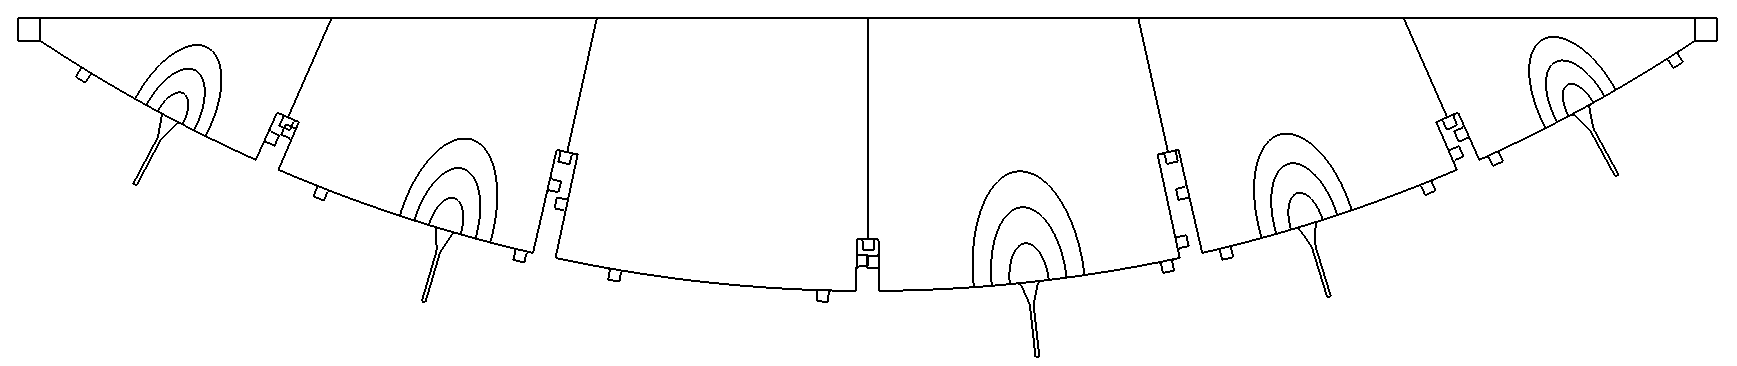
\includegraphics[width=473.38pt,height=100.5pt]{diagrams/placenta-geometry-diagrams/mesh_inverted-circle-slice-6-flat_normal-walls_septal-veins.png}};
%Shape: Polygon [id:ds599560967686122] 
\draw  [fill={rgb, 255:red, 155; green, 155; blue, 155 }  ,fill opacity=0.2 ] (436.42,180.33) -- (227,262.5) -- (215,262.5) -- (311.92,180.33) -- cycle ;
%Straight Lines [id:da3836552587833064] 
\draw [color={rgb, 255:red, 155; green, 155; blue, 155 }  ,draw opacity=1 ] [dash pattern={on 0.84pt off 2.51pt}]  (632.5,226.5) -- (632.5,345) ;
%Straight Lines [id:da8869549916108876] 
\draw [color={rgb, 255:red, 155; green, 155; blue, 155 }  ,draw opacity=1 ] [dash pattern={on 0.84pt off 2.51pt}]  (555,269) -- (555,345) ;
%Straight Lines [id:da08890647812691421] 
\draw [color={rgb, 255:red, 128; green, 128; blue, 128 }  ,draw opacity=1 ]   (558,345) -- (629.5,345) ;
\draw [shift={(632.5,345)}, rotate = 180] [fill={rgb, 255:red, 128; green, 128; blue, 128 }  ,fill opacity=1 ][line width=0.08]  [draw opacity=0] (7.14,-3.43) -- (0,0) -- (7.14,3.43) -- cycle    ;
\draw [shift={(555,345)}, rotate = 0] [fill={rgb, 255:red, 128; green, 128; blue, 128 }  ,fill opacity=1 ][line width=0.08]  [draw opacity=0] (7.14,-3.43) -- (0,0) -- (7.14,3.43) -- cycle    ;
%Straight Lines [id:da4569539433423251] 
\draw [color={rgb, 255:red, 155; green, 155; blue, 155 }  ,draw opacity=1 ] [dash pattern={on 0.84pt off 2.51pt}]  (545.5,273) -- (545.5,345) ;
%Straight Lines [id:da6425775020756577] 
\draw [color={rgb, 255:red, 155; green, 155; blue, 155 }  ,draw opacity=1 ] [dash pattern={on 0.84pt off 2.51pt}]  (453,303.5) -- (453,345) ;
%Straight Lines [id:da84971523704646] 
\draw [color={rgb, 255:red, 155; green, 155; blue, 155 }  ,draw opacity=1 ] [dash pattern={on 0.84pt off 2.51pt}]  (445.5,303.5) -- (445.5,344) ;
%Straight Lines [id:da4522901839526503] 
\draw [color={rgb, 255:red, 155; green, 155; blue, 155 }  ,draw opacity=1 ] [dash pattern={on 0.84pt off 2.51pt}]  (334.5,316) -- (334.5,344) ;
%Straight Lines [id:da886100326010987] 
\draw [color={rgb, 255:red, 128; green, 128; blue, 128 }  ,draw opacity=1 ]   (337.5,345) -- (442,345) ;
\draw [shift={(445,345)}, rotate = 180] [fill={rgb, 255:red, 128; green, 128; blue, 128 }  ,fill opacity=1 ][line width=0.08]  [draw opacity=0] (7.14,-3.43) -- (0,0) -- (7.14,3.43) -- cycle    ;
\draw [shift={(334.5,345)}, rotate = 0] [fill={rgb, 255:red, 128; green, 128; blue, 128 }  ,fill opacity=1 ][line width=0.08]  [draw opacity=0] (7.14,-3.43) -- (0,0) -- (7.14,3.43) -- cycle    ;
%Straight Lines [id:da2739622055496771] 
\draw [color={rgb, 255:red, 155; green, 155; blue, 155 }  ,draw opacity=1 ] [dash pattern={on 0.84pt off 2.51pt}]  (28.5,226.5) -- (28.5,345) ;
%Straight Lines [id:da8223757430798608] 
\draw [color={rgb, 255:red, 155; green, 155; blue, 155 }  ,draw opacity=1 ] [dash pattern={on 0.84pt off 2.51pt}]  (105.87,269.5) -- (105.87,345) ;
%Straight Lines [id:da9585020997428355] 
\draw [color={rgb, 255:red, 128; green, 128; blue, 128 }  ,draw opacity=1 ]   (102.87,345) -- (31.5,345) ;
\draw [shift={(28.5,345)}, rotate = 360] [fill={rgb, 255:red, 128; green, 128; blue, 128 }  ,fill opacity=1 ][line width=0.08]  [draw opacity=0] (7.14,-3.43) -- (0,0) -- (7.14,3.43) -- cycle    ;
\draw [shift={(105.87,345)}, rotate = 180] [fill={rgb, 255:red, 128; green, 128; blue, 128 }  ,fill opacity=1 ][line width=0.08]  [draw opacity=0] (7.14,-3.43) -- (0,0) -- (7.14,3.43) -- cycle    ;
%Straight Lines [id:da7396996741803523] 
\draw [color={rgb, 255:red, 155; green, 155; blue, 155 }  ,draw opacity=1 ] [dash pattern={on 0.84pt off 2.51pt}]  (115.35,273) -- (115.35,345) ;
%Straight Lines [id:da7690060794723255] 
\draw [color={rgb, 255:red, 155; green, 155; blue, 155 }  ,draw opacity=1 ] [dash pattern={on 0.84pt off 2.51pt}]  (207.7,303) -- (207.7,345) ;
%Straight Lines [id:da1750801006916194] 
\draw [color={rgb, 255:red, 155; green, 155; blue, 155 }  ,draw opacity=1 ] [dash pattern={on 0.84pt off 2.51pt}]  (215.19,305) -- (215.19,344) ;
%Straight Lines [id:da36519166335869224] 
\draw [color={rgb, 255:red, 155; green, 155; blue, 155 }  ,draw opacity=1 ] [dash pattern={on 0.84pt off 2.51pt}]  (326,316.5) -- (326,344) ;
%Straight Lines [id:da5227117484890365] 
\draw [color={rgb, 255:red, 128; green, 128; blue, 128 }  ,draw opacity=1 ]   (323,345) -- (218.69,345) ;
\draw [shift={(215.69,345)}, rotate = 360] [fill={rgb, 255:red, 128; green, 128; blue, 128 }  ,fill opacity=1 ][line width=0.08]  [draw opacity=0] (7.14,-3.43) -- (0,0) -- (7.14,3.43) -- cycle    ;
\draw [shift={(326,345)}, rotate = 180] [fill={rgb, 255:red, 128; green, 128; blue, 128 }  ,fill opacity=1 ][line width=0.08]  [draw opacity=0] (7.14,-3.43) -- (0,0) -- (7.14,3.43) -- cycle    ;
%Straight Lines [id:da9869684148666715] 
\draw [color={rgb, 255:red, 128; green, 128; blue, 128 }  ,draw opacity=1 ]   (204.2,345) -- (118.35,345) ;
\draw [shift={(115.35,345)}, rotate = 360] [fill={rgb, 255:red, 128; green, 128; blue, 128 }  ,fill opacity=1 ][line width=0.08]  [draw opacity=0] (7.14,-3.43) -- (0,0) -- (7.14,3.43) -- cycle    ;
\draw [shift={(207.2,345)}, rotate = 180] [fill={rgb, 255:red, 128; green, 128; blue, 128 }  ,fill opacity=1 ][line width=0.08]  [draw opacity=0] (7.14,-3.43) -- (0,0) -- (7.14,3.43) -- cycle    ;
%Shape: Rectangle [id:dp7784307888916284] 
\draw   (379,303.5) -- (396.5,303.5) -- (396.5,341.5) -- (379,341.5) -- cycle ;
%Shape: Rectangle [id:dp7413532166529391] 
\draw   (18,215.27) -- (35.5,215.27) -- (35.5,228.77) -- (18,228.77) -- cycle ;
%Shape: Rectangle [id:dp1083356594712217] 
\draw   (305.17,310.67) -- (322.67,310.67) -- (322.67,326.17) -- (305.17,326.17) -- cycle ;
%Shape: Polygon [id:ds13903772067200593] 
\draw  [fill={rgb, 255:red, 155; green, 155; blue, 155 }  ,fill opacity=0.2 ] (635,183) -- (396.5,303.5) -- (379,303.5) -- (463.75,183) -- cycle ;
%Shape: Polygon [id:ds6960752336656928] 
\draw  [fill={rgb, 255:red, 155; green, 155; blue, 155 }  ,fill opacity=0.2 ] (139.25,187.75) -- (35.5,215.27) -- (18,215.27) -- (14.75,187.75) -- cycle ;
%Shape: Polygon [id:ds16525050807756858] 
\draw  [fill={rgb, 255:red, 155; green, 155; blue, 155 }  ,fill opacity=0.2 ] (436.42,180.33) -- (322.67,310.67) -- (305.17,310.67) -- (311.92,180.33) -- cycle ;
%Shape: Rectangle [id:dp6070840373099016] 
\draw  [color={rgb, 255:red, 208; green, 2; blue, 27 }  ,draw opacity=1 ][fill={rgb, 255:red, 255; green, 255; blue, 255 }  ,fill opacity=1 ][line width=2.25] [blur shadow={shadow xshift=0pt,shadow yshift=0pt, shadow blur radius=1.5pt, shadow blur steps=4 ,shadow opacity=100}] (463.75,22.5) -- (635,22.5) -- (635,183) -- (463.75,183) -- cycle ;
%Image [id:dp7341682961381069] 
\draw (523.25,97.77) node  {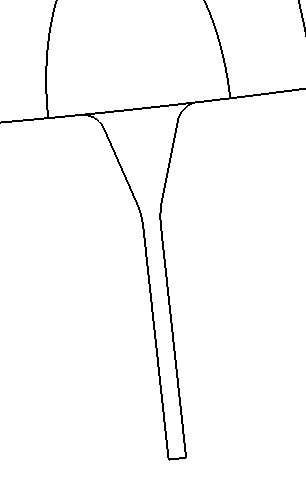
\includegraphics[width=54.75pt,height=89.28pt]{diagrams/placenta-geometry-diagrams/mesh_inverted-circle-slice-6-flat_normal-walls-septal-veins_artery.png}};
%Straight Lines [id:da2560686325124286] 
\draw [color={rgb, 255:red, 155; green, 155; blue, 155 }  ,draw opacity=1 ] [dash pattern={on 0.84pt off 2.51pt}]  (532.75,63) -- (575,57.75) ;
%Straight Lines [id:da862538474933769] 
\draw [color={rgb, 255:red, 155; green, 155; blue, 155 }  ,draw opacity=1 ] [dash pattern={on 0.84pt off 2.51pt}]  (531.25,150.75) -- (585.75,143.5) ;
%Straight Lines [id:da07631904575656989] 
\draw [color={rgb, 255:red, 128; green, 128; blue, 128 }  ,draw opacity=1 ]   (585.36,137.02) -- (575.64,61.98) ;
\draw [shift={(575.25,59)}, rotate = 82.61] [fill={rgb, 255:red, 128; green, 128; blue, 128 }  ,fill opacity=1 ][line width=0.08]  [draw opacity=0] (7.14,-3.43) -- (0,0) -- (7.14,3.43) -- cycle    ;
\draw [shift={(585.75,140)}, rotate = 262.61] [fill={rgb, 255:red, 128; green, 128; blue, 128 }  ,fill opacity=1 ][line width=0.08]  [draw opacity=0] (7.14,-3.43) -- (0,0) -- (7.14,3.43) -- cycle    ;
%Straight Lines [id:da9334742103638392] 
\draw [color={rgb, 255:red, 128; green, 128; blue, 128 }  ,draw opacity=1 ]   (526.19,150.18) -- (492.5,129.5) ;
\draw [shift={(528.75,151.75)}, rotate = 211.54] [fill={rgb, 255:red, 128; green, 128; blue, 128 }  ,fill opacity=1 ][line width=0.08]  [draw opacity=0] (6.25,-3) -- (0,0) -- (6.25,3) -- cycle    ;
%Straight Lines [id:da644000948100526] 
\draw [color={rgb, 255:red, 128; green, 128; blue, 128 }  ,draw opacity=1 ]   (535.18,86.02) -- (533.07,65.98) ;
\draw [shift={(532.75,63)}, rotate = 83.96] [fill={rgb, 255:red, 128; green, 128; blue, 128 }  ,fill opacity=1 ][line width=0.08]  [draw opacity=0] (5.36,-2.57) -- (0,0) -- (5.36,2.57) -- cycle    ;
\draw [shift={(535.5,89)}, rotate = 263.96] [fill={rgb, 255:red, 128; green, 128; blue, 128 }  ,fill opacity=1 ][line width=0.08]  [draw opacity=0] (5.36,-2.57) -- (0,0) -- (5.36,2.57) -- cycle    ;
%Straight Lines [id:da058958443439840025] 
\draw [color={rgb, 255:red, 155; green, 155; blue, 155 }  ,draw opacity=1 ] [dash pattern={on 0.84pt off 2.51pt}]  (526,89.75) -- (535.5,89) ;
%Straight Lines [id:da635774139796158] 
\draw [color={rgb, 255:red, 128; green, 128; blue, 128 }  ,draw opacity=1 ]   (528.02,57.33) -- (509.23,59.42) ;
\draw [shift={(506.25,59.75)}, rotate = 353.66] [fill={rgb, 255:red, 128; green, 128; blue, 128 }  ,fill opacity=1 ][line width=0.08]  [draw opacity=0] (5.36,-2.57) -- (0,0) -- (5.36,2.57) -- cycle    ;
\draw [shift={(531,57)}, rotate = 173.66] [fill={rgb, 255:red, 128; green, 128; blue, 128 }  ,fill opacity=1 ][line width=0.08]  [draw opacity=0] (5.36,-2.57) -- (0,0) -- (5.36,2.57) -- cycle    ;
%Shape: Rectangle [id:dp12087627646558885] 
\draw  [color={rgb, 255:red, 74; green, 144; blue, 226 }  ,draw opacity=1 ][fill={rgb, 255:red, 255; green, 255; blue, 255 }  ,fill opacity=1 ][line width=2.25] [blur shadow={shadow xshift=0pt,shadow yshift=0pt, shadow blur radius=1.5pt, shadow blur steps=4 ,shadow opacity=100}] (311.92,51.5) -- (436.42,51.5) -- (436.42,180.33) -- (311.92,180.33) -- cycle ;
%Image [id:dp11084122971065935] 
\draw (362.92,87.84) node  {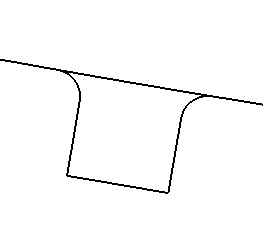
\includegraphics[width=56.25pt,height=51.76pt]{diagrams/placenta-geometry-diagrams/mesh_inverted-circle-slice-6-flat_normal-walls-septal-veins_vein.png}};
%Straight Lines [id:da4260411781736031] 
\draw [color={rgb, 255:red, 128; green, 128; blue, 128 }  ,draw opacity=1 ]   (371.2,114.18) -- (344.25,110.16) ;
\draw [shift={(341.28,109.72)}, rotate = 8.49] [fill={rgb, 255:red, 128; green, 128; blue, 128 }  ,fill opacity=1 ][line width=0.08]  [draw opacity=0] (5.36,-2.57) -- (0,0) -- (5.36,2.57) -- cycle    ;
\draw [shift={(374.17,114.63)}, rotate = 188.49] [fill={rgb, 255:red, 128; green, 128; blue, 128 }  ,fill opacity=1 ][line width=0.08]  [draw opacity=0] (5.36,-2.57) -- (0,0) -- (5.36,2.57) -- cycle    ;
%Straight Lines [id:da13622705064859697] 
\draw [color={rgb, 255:red, 128; green, 128; blue, 128 }  ,draw opacity=1 ]   (383.91,85.29) -- (380.42,105.63) ;
\draw [shift={(379.92,108.58)}, rotate = 279.73] [fill={rgb, 255:red, 128; green, 128; blue, 128 }  ,fill opacity=1 ][line width=0.08]  [draw opacity=0] (5.36,-2.57) -- (0,0) -- (5.36,2.57) -- cycle    ;
\draw [shift={(384.42,82.33)}, rotate = 99.73] [fill={rgb, 255:red, 128; green, 128; blue, 128 }  ,fill opacity=1 ][line width=0.08]  [draw opacity=0] (5.36,-2.57) -- (0,0) -- (5.36,2.57) -- cycle    ;
%Shape: Rectangle [id:dp043044360722185315] 
\draw  [color={rgb, 255:red, 74; green, 144; blue, 226 }  ,draw opacity=1 ][fill={rgb, 255:red, 255; green, 255; blue, 255 }  ,fill opacity=1 ][line width=2.25] [blur shadow={shadow xshift=0pt,shadow yshift=0pt, shadow blur radius=1.5pt, shadow blur steps=4 ,shadow opacity=100}] (14.75,110.5) -- (139.25,110.5) -- (139.25,187.75) -- (14.75,187.75) -- cycle ;
%Image [id:dp43909768466905374] 
\draw (88.25,149.86) node [xscale=-1] {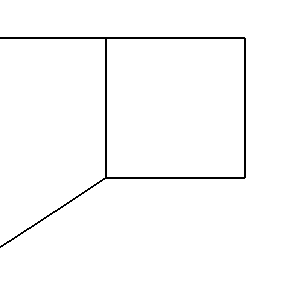
\includegraphics[width=52.5pt,height=53.05pt]{diagrams/placenta-geometry-diagrams/mesh_inverted-circle-slice-6-flat_normal-walls-septal-veins_marginal-sinus.png}};
%Straight Lines [id:da33088686310200743] 
\draw [color={rgb, 255:red, 128; green, 128; blue, 128 }  ,draw opacity=1 ]   (94,161.75) -- (66.75,161.75) ;
\draw [shift={(63.75,161.75)}, rotate = 360] [fill={rgb, 255:red, 128; green, 128; blue, 128 }  ,fill opacity=1 ][line width=0.08]  [draw opacity=0] (5.36,-2.57) -- (0,0) -- (5.36,2.57) -- cycle    ;
\draw [shift={(97,161.75)}, rotate = 180] [fill={rgb, 255:red, 128; green, 128; blue, 128 }  ,fill opacity=1 ][line width=0.08]  [draw opacity=0] (5.36,-2.57) -- (0,0) -- (5.36,2.57) -- cycle    ;
%Straight Lines [id:da3164833140775334] 
\draw [color={rgb, 255:red, 128; green, 128; blue, 128 }  ,draw opacity=1 ]   (57.75,125.5) -- (57.75,152.75) ;
\draw [shift={(57.75,155.75)}, rotate = 270] [fill={rgb, 255:red, 128; green, 128; blue, 128 }  ,fill opacity=1 ][line width=0.08]  [draw opacity=0] (5.36,-2.57) -- (0,0) -- (5.36,2.57) -- cycle    ;
\draw [shift={(57.75,122.5)}, rotate = 90] [fill={rgb, 255:red, 128; green, 128; blue, 128 }  ,fill opacity=1 ][line width=0.08]  [draw opacity=0] (5.36,-2.57) -- (0,0) -- (5.36,2.57) -- cycle    ;
%Shape: Rectangle [id:dp3214087399382912] 
\draw  [color={rgb, 255:red, 65; green, 117; blue, 5 }  ,draw opacity=1 ][dash pattern={on 2.53pt off 3.02pt}][line width=2.25]  (264.5,303) -- (281.5,303) -- (281.5,320) -- (264.5,320) -- cycle ;
%Shape: Axis 2D [id:dp5493960903283415] 
\draw  (10.68,368.48) -- (43.48,368.48)(13.96,338.96) -- (13.96,371.76) (36.48,363.48) -- (43.48,368.48) -- (36.48,373.48) (8.96,345.96) -- (13.96,338.96) -- (18.96,345.96)  ;

%Straight Lines [id:da8673543563072263] 
\draw [color={rgb, 255:red, 65; green, 117; blue, 5 }  ,draw opacity=1 ]   (244.5,173) -- (273.01,293.58) ;
\draw [shift={(273.7,296.5)}, rotate = 256.7] [fill={rgb, 255:red, 65; green, 117; blue, 5 }  ,fill opacity=1 ][line width=0.08]  [draw opacity=0] (8.93,-4.29) -- (0,0) -- (8.93,4.29) -- cycle    ;
%Straight Lines [id:da15777572686334396] 
\draw [color={rgb, 255:red, 128; green, 128; blue, 128 }  ,draw opacity=1 ]   (456.5,345) -- (542.5,345) ;
\draw [shift={(545.5,345)}, rotate = 180] [fill={rgb, 255:red, 128; green, 128; blue, 128 }  ,fill opacity=1 ][line width=0.08]  [draw opacity=0] (7.14,-3.43) -- (0,0) -- (7.14,3.43) -- cycle    ;
\draw [shift={(453.5,345)}, rotate = 0] [fill={rgb, 255:red, 128; green, 128; blue, 128 }  ,fill opacity=1 ][line width=0.08]  [draw opacity=0] (7.14,-3.43) -- (0,0) -- (7.14,3.43) -- cycle    ;
%Straight Lines [id:da20967786638483576] 
\draw [color={rgb, 255:red, 128; green, 128; blue, 128 }  ,draw opacity=1 ]   (126.53,260.24) -- (121.97,270.51) ;
\draw [shift={(120.75,273.25)}, rotate = 293.96] [fill={rgb, 255:red, 128; green, 128; blue, 128 }  ,fill opacity=1 ][line width=0.08]  [draw opacity=0] (3.57,-1.72) -- (0,0) -- (3.57,1.72) -- cycle    ;
\draw [shift={(127.75,257.5)}, rotate = 113.96] [fill={rgb, 255:red, 128; green, 128; blue, 128 }  ,fill opacity=1 ][line width=0.08]  [draw opacity=0] (3.57,-1.72) -- (0,0) -- (3.57,1.72) -- cycle    ;
%Straight Lines [id:da999991789814658] 
\draw [color={rgb, 255:red, 128; green, 128; blue, 128 }  ,draw opacity=1 ]   (228.14,272.19) -- (222.1,301.15) ;
\draw [shift={(221.49,304.09)}, rotate = 281.77] [fill={rgb, 255:red, 128; green, 128; blue, 128 }  ,fill opacity=1 ][line width=0.08]  [draw opacity=0] (3.57,-1.72) -- (0,0) -- (3.57,1.72) -- cycle    ;
\draw [shift={(228.75,269.25)}, rotate = 101.77] [fill={rgb, 255:red, 128; green, 128; blue, 128 }  ,fill opacity=1 ][line width=0.08]  [draw opacity=0] (3.57,-1.72) -- (0,0) -- (3.57,1.72) -- cycle    ;
%Shape: Rectangle [id:dp842610769802747] 
\draw   (215,262.5) -- (227,262.5) -- (227,272.5) -- (215,272.5) -- cycle ;
%Shape: Rectangle [id:dp34481258515956204] 
\draw  [color={rgb, 255:red, 65; green, 117; blue, 5 }  ,draw opacity=1 ][dash pattern={on 2.53pt off 3.02pt}][line width=2.25]  (94,260.5) -- (106,260.5) -- (106,272) -- (94,272) -- cycle ;
%Straight Lines [id:da484653672836302] 
\draw [color={rgb, 255:red, 65; green, 117; blue, 5 }  ,draw opacity=1 ]   (187.5,196.5) -- (107.93,254.24) ;
\draw [shift={(105.5,256)}, rotate = 324.03] [fill={rgb, 255:red, 65; green, 117; blue, 5 }  ,fill opacity=1 ][line width=0.08]  [draw opacity=0] (8.93,-4.29) -- (0,0) -- (8.93,4.29) -- cycle    ;

% Text Node
\draw (67.18,348.4) node [anchor=north] [inner sep=0.75pt]  [font=\footnotesize,color={rgb, 255:red, 128; green, 128; blue, 128 }  ,opacity=1 ]  {$28.65\ \text{mm}$};
% Text Node
\draw (161.28,348.4) node [anchor=north] [inner sep=0.75pt]  [font=\footnotesize,color={rgb, 255:red, 128; green, 128; blue, 128 }  ,opacity=1 ]  {$33.85\ \text{mm}$};
% Text Node
\draw (270.84,348.4) node [anchor=north] [inner sep=0.75pt]  [font=\footnotesize,color={rgb, 255:red, 128; green, 128; blue, 128 }  ,opacity=1 ]  {$40\ \text{mm}$};
% Text Node
\draw (389.75,348.4) node [anchor=north] [inner sep=0.75pt]  [font=\footnotesize,color={rgb, 255:red, 128; green, 128; blue, 128 }  ,opacity=1 ]  {$40\ \text{mm}$};
% Text Node
\draw (499.5,348.4) node [anchor=north] [inner sep=0.75pt]  [font=\footnotesize,color={rgb, 255:red, 128; green, 128; blue, 128 }  ,opacity=1 ]  {$33.85\ \text{mm}$};
% Text Node
\draw (593.75,348.4) node [anchor=north] [inner sep=0.75pt]  [font=\footnotesize,color={rgb, 255:red, 128; green, 128; blue, 128 }  ,opacity=1 ]  {$28.65\ \text{mm}$};
% Text Node
\draw (582.5,99.5) node [anchor=west] [inner sep=0.75pt]  [font=\footnotesize,color={rgb, 255:red, 128; green, 128; blue, 128 }  ,opacity=1 ]  {$10\ \text{mm}$};
% Text Node
\draw (512.64,126.72) node [anchor=south east] [inner sep=0.75pt]  [font=\scriptsize,color={rgb, 255:red, 128; green, 128; blue, 128 }  ,opacity=1 ]  {$0.5\ \text{mm}$};
% Text Node
\draw (536.13,76) node [anchor=west] [inner sep=0.75pt]  [font=\scriptsize,color={rgb, 255:red, 128; green, 128; blue, 128 }  ,opacity=1 ]  {$3\ \text{mm}$};
% Text Node
\draw (518.63,54.98) node [anchor=south] [inner sep=0.75pt]  [font=\scriptsize,color={rgb, 255:red, 128; green, 128; blue, 128 }  ,opacity=1 ]  {$2.4\ \text{mm}$};
% Text Node
\draw (80.38,165.15) node [anchor=north] [inner sep=0.75pt]  [font=\scriptsize,color={rgb, 255:red, 128; green, 128; blue, 128 }  ,opacity=1 ]  {$3\ \text{mm}$};
% Text Node
\draw (55.75,139.13) node [anchor=east] [inner sep=0.75pt]  [font=\scriptsize,color={rgb, 255:red, 128; green, 128; blue, 128 }  ,opacity=1 ]  {$3\ \text{mm}$};
% Text Node
\draw (357.22,115.53) node [anchor=north] [inner sep=0.75pt]  [font=\scriptsize,color={rgb, 255:red, 128; green, 128; blue, 128 }  ,opacity=1 ,rotate=-8.49]  {$1.5\ \text{mm}$};
% Text Node
\draw (384.14,95.75) node [anchor=west] [inner sep=0.75pt]  [font=\scriptsize,color={rgb, 255:red, 128; green, 128; blue, 128 }  ,opacity=1 ,rotate=-8.49]  {$1.5\ \text{mm}$};
% Text Node
\draw (46.86,365) node [anchor=west] [inner sep=0.75pt]  [font=\footnotesize]  {$x$};
% Text Node
\draw (15,332.55) node [anchor=south] [inner sep=0.75pt]  [font=\footnotesize]  {$y$};
% Text Node
\draw (373.4,139.41) node [anchor=north] [inner sep=0.75pt]  [font=\small] [align=left] {\textcolor[rgb]{0.29,0.56,0.89}{basal plate and}\\\textcolor[rgb]{0.29,0.56,0.89}{septal wall veins}};
% Text Node
\draw (545.5,174.4) node [anchor=south] [inner sep=0.75pt]  [font=\small,color={rgb, 255:red, 208; green, 2; blue, 27 }  ,opacity=1 ] [align=left] {spiral artery};
% Text Node
\draw (126.02,266.74) node [anchor=west] [inner sep=0.75pt]  [font=\tiny,color={rgb, 255:red, 128; green, 128; blue, 128 }  ,opacity=1 ,rotate=-23.4]  {$6.90\ \text{mm}$};
% Text Node
\draw (227.07,287.11) node [anchor=west] [inner sep=0.75pt]  [font=\tiny,color={rgb, 255:red, 128; green, 128; blue, 128 }  ,opacity=1 ,rotate=-12.55]  {$14.07\ \text{mm}$};
% Text Node
\draw (202.23,156.01) node [anchor=north west][inner sep=0.75pt]  [font=\small,color={rgb, 255:red, 65; green, 117; blue, 5 }  ,opacity=1 ] [align=left] {omitted artery};
% Text Node
\draw (153.73,179.51) node [anchor=north west][inner sep=0.75pt]  [font=\small,color={rgb, 255:red, 65; green, 117; blue, 5 }  ,opacity=1 ] [align=left] {omitted vein};


\end{tikzpicture}

            \figureretag{fig:inverted-circle-slice-6-flat:dimensions}
            \caption{Diagram illustrating our 2D placenta geometry repeated from \S\ref{sec:modelling:geometries:2d-placenta}.}
        \end{figure}
    
        Throughout \S\ref{sec:nutrient-uptake:variation-of-vessels}, we will fix all parameter values from Tables \ref{tab:structural-parameters} and \ref{tab:problem-parameters}, and instead vary both the number and position of the arteries and veins. We vary uniformly-at-random the number and position of all arteries and veins, up to a maximum of $N_\text{A} = 6$ arteries (one per placentone) and $N_\text{V} = 27$ veins (2 per placentone, 3 per wall), where for simplicity we retain the $2$ larger marginal sinus veins in all simulations. The positions of arteries and veins are constrained to avoid overlap, and so that the central cavity associated with every given artery does not intersect with the chorionic plate and septal walls. Figure \ref{fig:inverted-circle-slice-6-flat:dimensions} (repeated here from \S\ref{sec:modelling:geometries:2d-placenta}) shows a sketch of an example domain illustrating the ways in which various arteries and veins may appear. The proceeding results are obtained from an ensemble of $N_\text{sim} = 1000$ realisations\footnote{An additional $100$ simulations are run specifically for $N_\text{A} = 6$ and $N_\text{V} = 27$ to ensure that there is a sufficiently large sample size for when we consider subsets of the data.} of the computational domain as described in Algorithm \ref{alg:generate-vessels}, where $\mathcal{U}(a, b)$ denotes the discrete uniform distribution, and $L, T, R$ respectively denote a `left', `top', and `right' position; $L,T,R \in \{0, 1\}$ and are used in the tuples on line 4 of Algorithm \ref{alg:generate-vessels} to denote chosen left and right veins on the basal plate of each placentone, and chosen left, top, and right veins on each septal wall. A `$0$' denotes a vein that is omitted, and a `$1$' denotes a vein that is present.

        \begin{algorithm}
            \For{$n=1$ \KwTo $N_\text{sim}$}{
                Sample $N_\text{A} \sim \mathcal{U}(1, 6)$ \\
                Sample $N_\text{V} \sim \mathcal{U}(0, 27)$ \\
                Uniformly-at-random select:
                \begin{itemize}
                    \item Number of arteries $n^i_\text{a} \in \{0, 1\}$ per placentone
                    \item Number of basal plate veins $n^{i}_\text{bp} = (L, R); L, R \in \{0, 1\}$ per placentone
                    \item Number of septal wall veins $n^{j}_\text{sw} = (L, T, R); L, T, R \in \{0, 1\}$ per wall
                \end{itemize}
                subject to $\sum_{i=1}^6 n^i_\text{a} = N_\text{A}$ and $\sum_{i=1}^6 |n^i_\text{bp}| + \sum_{j=1}^5 |n^j_\text{sw}| = N_\text{V}$ \\ \nl
                \For{$i=1$ \KwTo $6$ placentones}{
                    Place $n^i_\text{a}$ at continuously uniformly random positions along basal plate, such that:
                    \begin{itemize}
                        \item There is room for left and right basal plate veins, if they exist
                        \item There is room for the central cavity
                    \end{itemize} \nl
                    Place $n^i_\text{bp}$ at continuously uniformly random positions in the remaining space
                } \nl
                \For{$j=1$ \KwTo $5$ walls}{
                    Place $n^i_\text{sw}$ at continuously uniformly random positions along the left side, top, and right side of septal walls
                } \nl
                Generate mesh $\mathcal{T}_h$ with selected vessels and positions \\ \nl
                Compute $\vec{u}_h$ and $c_h$ from simulation, and compute all seven measures of placental efficiency%
            }%
            \caption{Algorithm to generate $N_\text{sim}$ simulations with varying numbers and positions of vessels.}%
            \label{alg:generate-vessels}
        \end{algorithm}

        Figures \ref{fig:mega-vessels1}--\ref{fig:mega-vessels5} present the main results of \S\ref{sec:nutrient-uptake:variation-of-vessels} for all seven efficiency measures, which we will discuss in depth throughout the remainder of \S\ref{sec:nutrient-uptake:variation-of-vessels}. We highlight that each individual graph presents data for the \textit{same} ensemble of simulations, but are visualised in several different ways.
        
        \subsection{Effects on \texorpdfstring{$\bar{v}(\Omega_\text{IVS})$}{average IVS speed} and \texorpdfstring{$\bar{c}$}{average oxygen concentration}} \label{sec:nutrient-uptake:average-velocity-and-concentration}
            We first discuss the influence of these structural variations on flow and oxygen uptake, as measured by $\bar{v}(\Omega_\text{IVS})$ and $\bar{c}$ (Equations \eqref{eq:eff-v} and \eqref{eq:eff-c}). We note that we have selected $\Omega_\text{IVS}$ in which to calculate $\bar{v}$, as flow in the central cavity can be much faster \cite{lecarpentierComputationalFluidDynamic2016}. Figure \ref{fig:mega-vessels1} summarises the results from all $N_\text{sim}$ simulations. Figure \ref{fig:mega-vessels1:results} shows the median values of $\bar{v}(\Omega_\text{IVS})$ and $\bar{c}$ obtained from our ensemble, plotted as a dashed blue line as a function of $N_\text{A}$, $N_\text{V}$, and the ratio $N_\text{V}/N_\text{A}$. The shaded region surrounding the median corresponds to the area between the $25$th and $75$th percentile of the data (i.e., the interquartile range). Individual outlier points are plotted outside this region. Orange lines denote subsets of the data, as indicated in the inset legends. We re-emphasise that the positions of the vessels are random and do not correlate to the choice of the number of vessels on the horizontal axes. The coloured crosses indicate specific realisations, for which we visualise the corresponding velocity and oxygen concentration fields in Figure \ref{fig:mega-vessels1:simulations}. These specific realisations are chosen in large part to demonstrate extreme choices in the number of vessels.

            \begin{figure}
                % Date generated: 2024-05-18 17:35:33
                % Commit: eac341b1ef691c92e8badeb0786f784648653b40
                % File run: ./drivers/variations_2024-03-21/vary_mega-vessels.py
                \centering
                \begin{subfigure}{\textwidth}
                    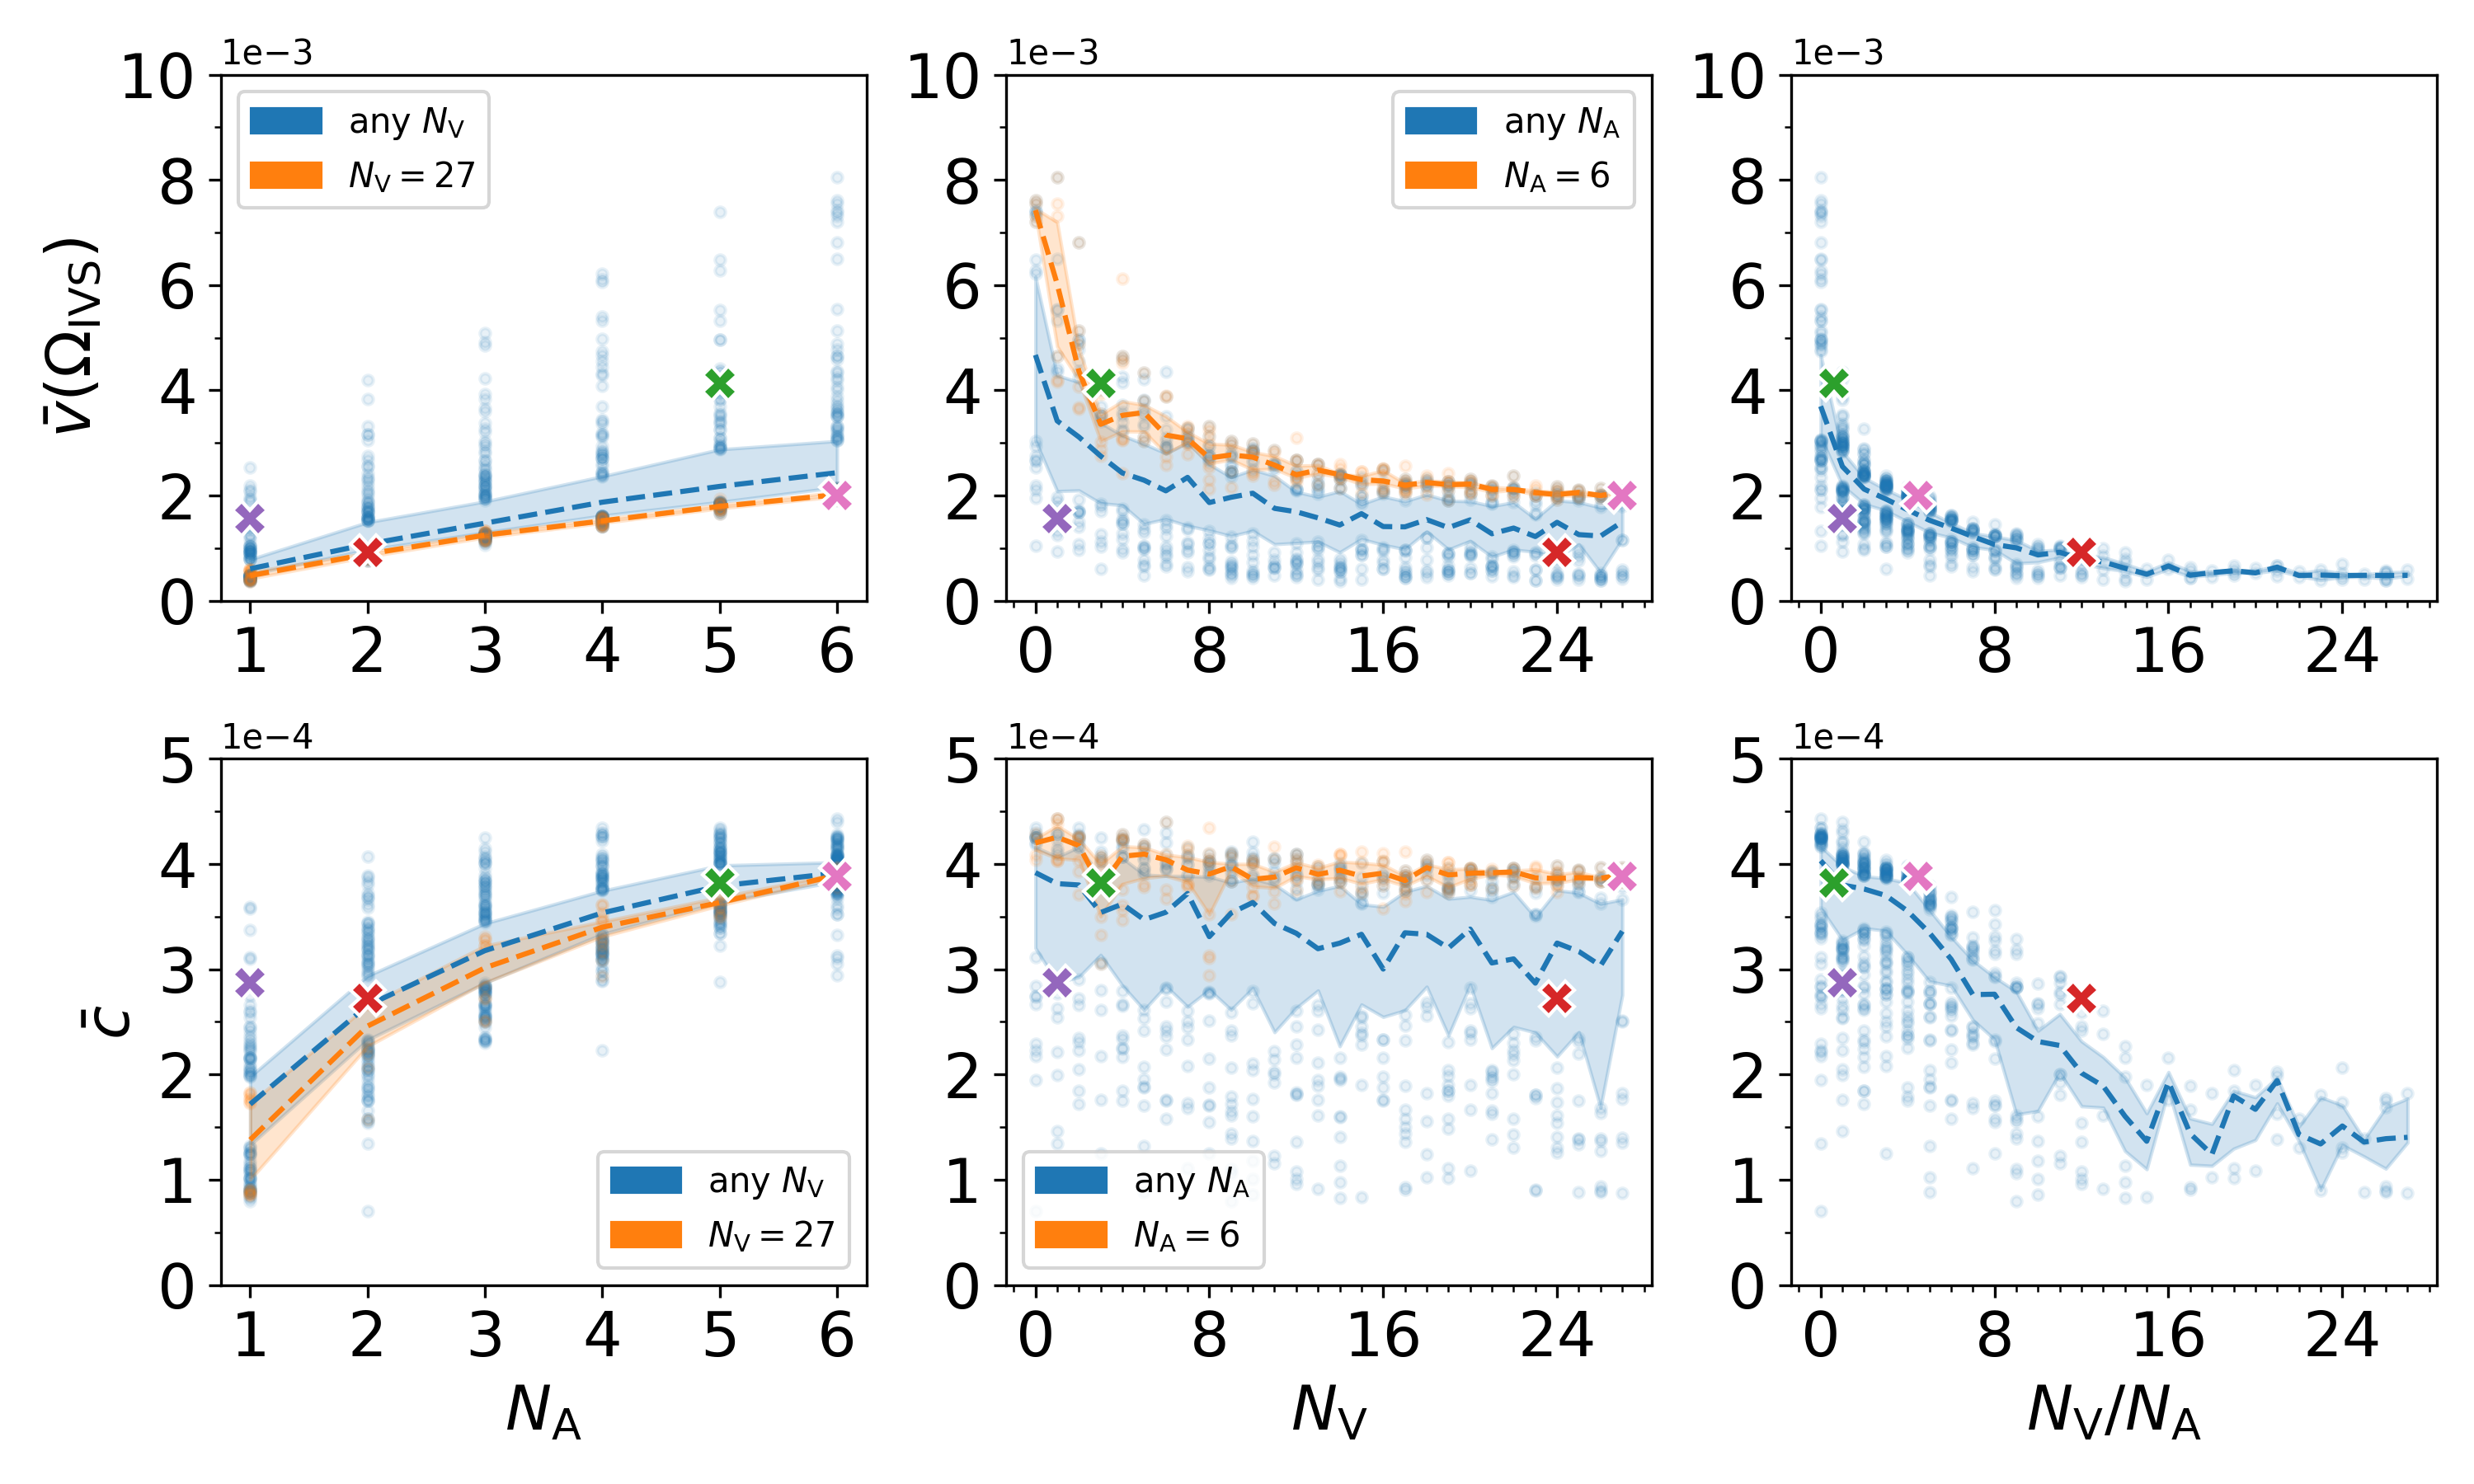
\includegraphics[width=\textwidth]{diagrams/results-variations/mega1_no-arteries_no-veins_veins-to-arteries.png}
                    \caption{}
                    \label{fig:mega-vessels1:results}
                \end{subfigure}
                \par\bigskip\bigskip
                \begin{subfigure}{\textwidth}
                    

\tikzset{every picture/.style={line width=0.75pt}} %set default line width to 0.75pt        

\begin{tikzpicture}[x=0.75pt,y=0.75pt,yscale=-1,xscale=1]
%uncomment if require: \path (0,319); %set diagram left start at 0, and has height of 319

%Shape: Rectangle [id:dp5853281871424232] 
\draw  [color={rgb, 255:red, 0; green, 128; blue, 2 }  ,draw opacity=1 ][line width=3.75]  (10.8,134.17) -- (330.77,134.17) -- (330.77,255) -- (10.8,255) -- cycle ;
%Shape: Rectangle [id:dp0668476806187166] 
\draw  [color={rgb, 255:red, 116; green, 73; blue, 156 }  ,draw opacity=1 ][line width=3.75]  (10.77,9.84) -- (330.44,9.84) -- (330.44,129) -- (10.77,129) -- cycle ;
%Shape: Rectangle [id:dp8412963857367168] 
\draw  [color={rgb, 255:red, 179; green, 0; blue, 2 }  ,draw opacity=1 ][line width=3.75]  (335.52,9.84) -- (655.19,9.84) -- (655.19,129) -- (335.52,129) -- cycle ;
%Shape: Rectangle [id:dp403011712811292] 
\draw  [color={rgb, 255:red, 192; green, 89; blue, 161 }  ,draw opacity=1 ][line width=3.75]  (335.75,134.09) -- (655.42,134.09) -- (655.42,255) -- (335.75,255) -- cycle ;
%Image [id:dp4663100234222186] 
\draw (135.5,43.75) node  {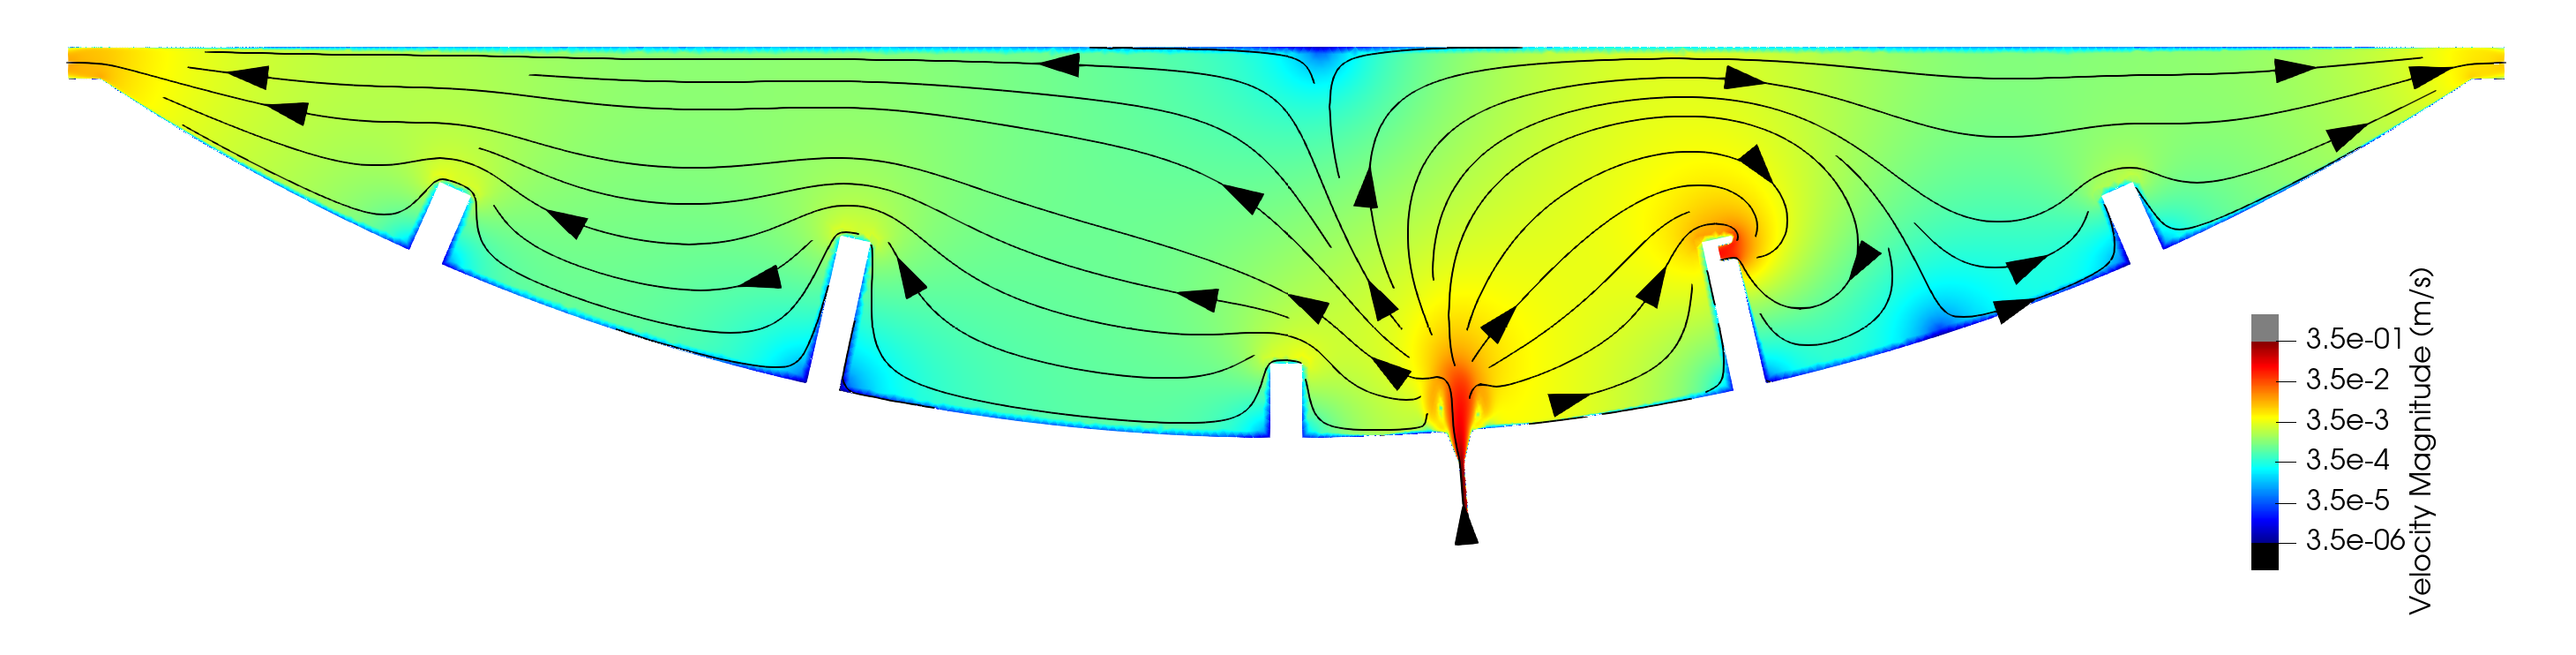
\includegraphics[width=181.5pt,height=46.12pt]{diagrams/results-variations/70-velocity.png}};
%Image [id:dp3190773005750116] 
\draw (135.01,98.75) node  {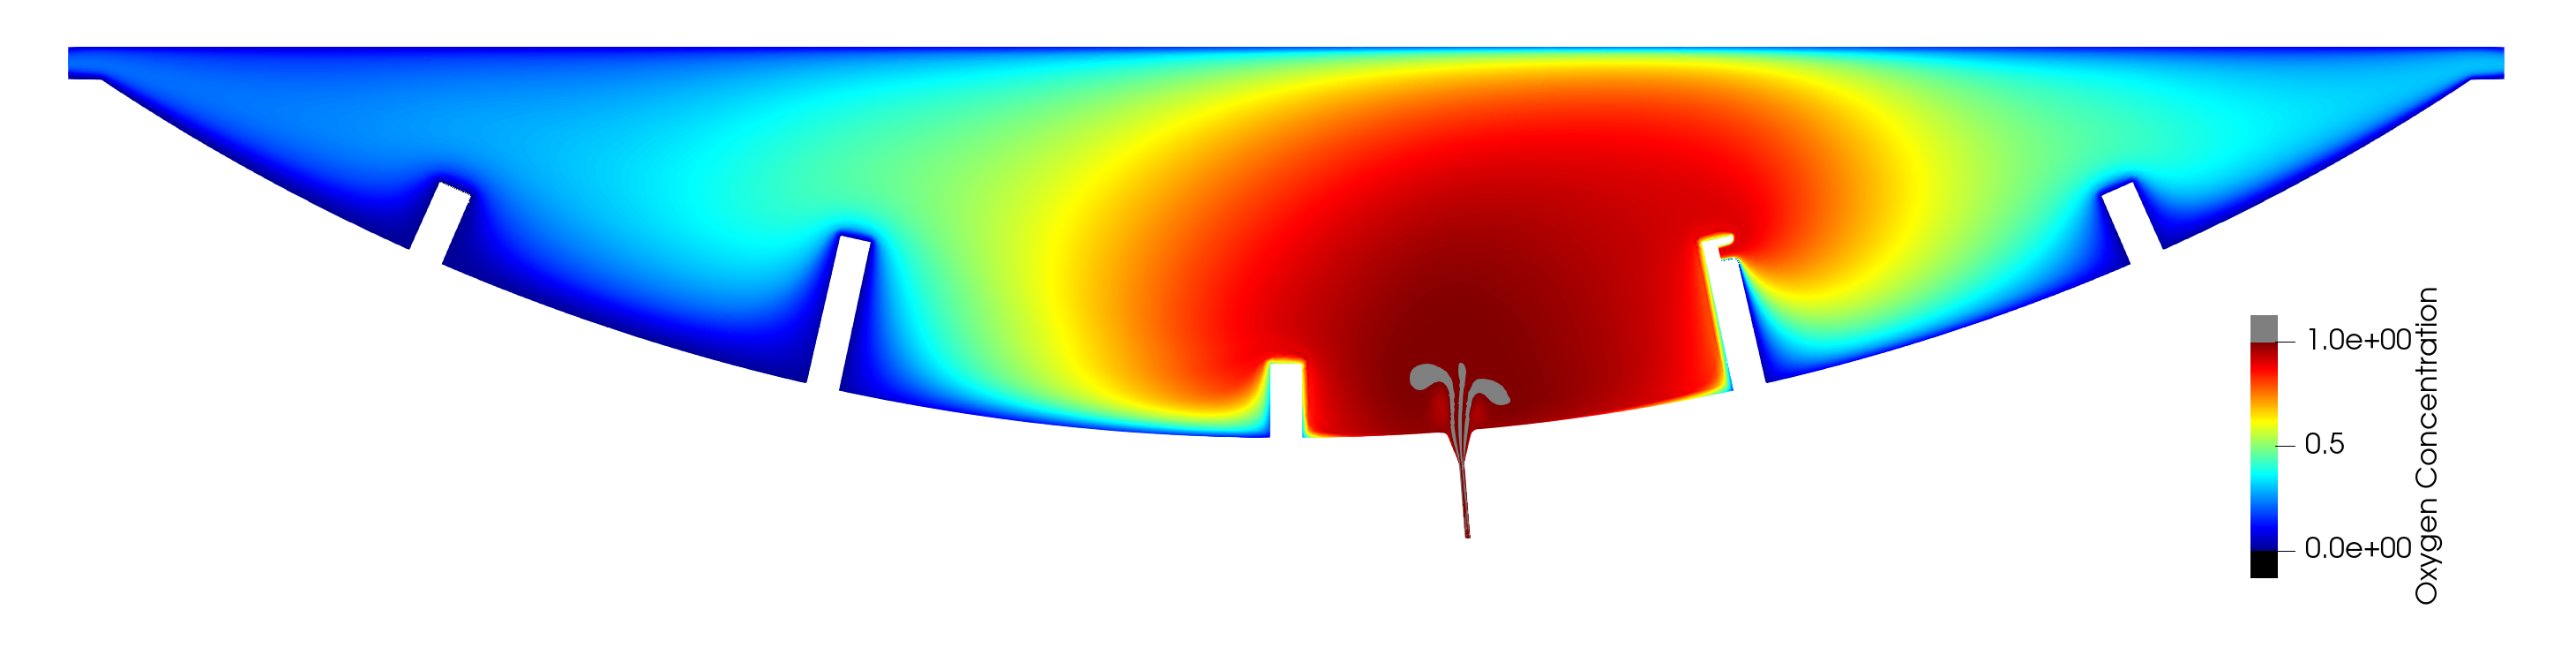
\includegraphics[width=181.52pt,height=46.13pt]{diagrams/results-variations/70-oxygen.png}};
%Image [id:dp5209728544208736] 
\draw (462,43.25) node  {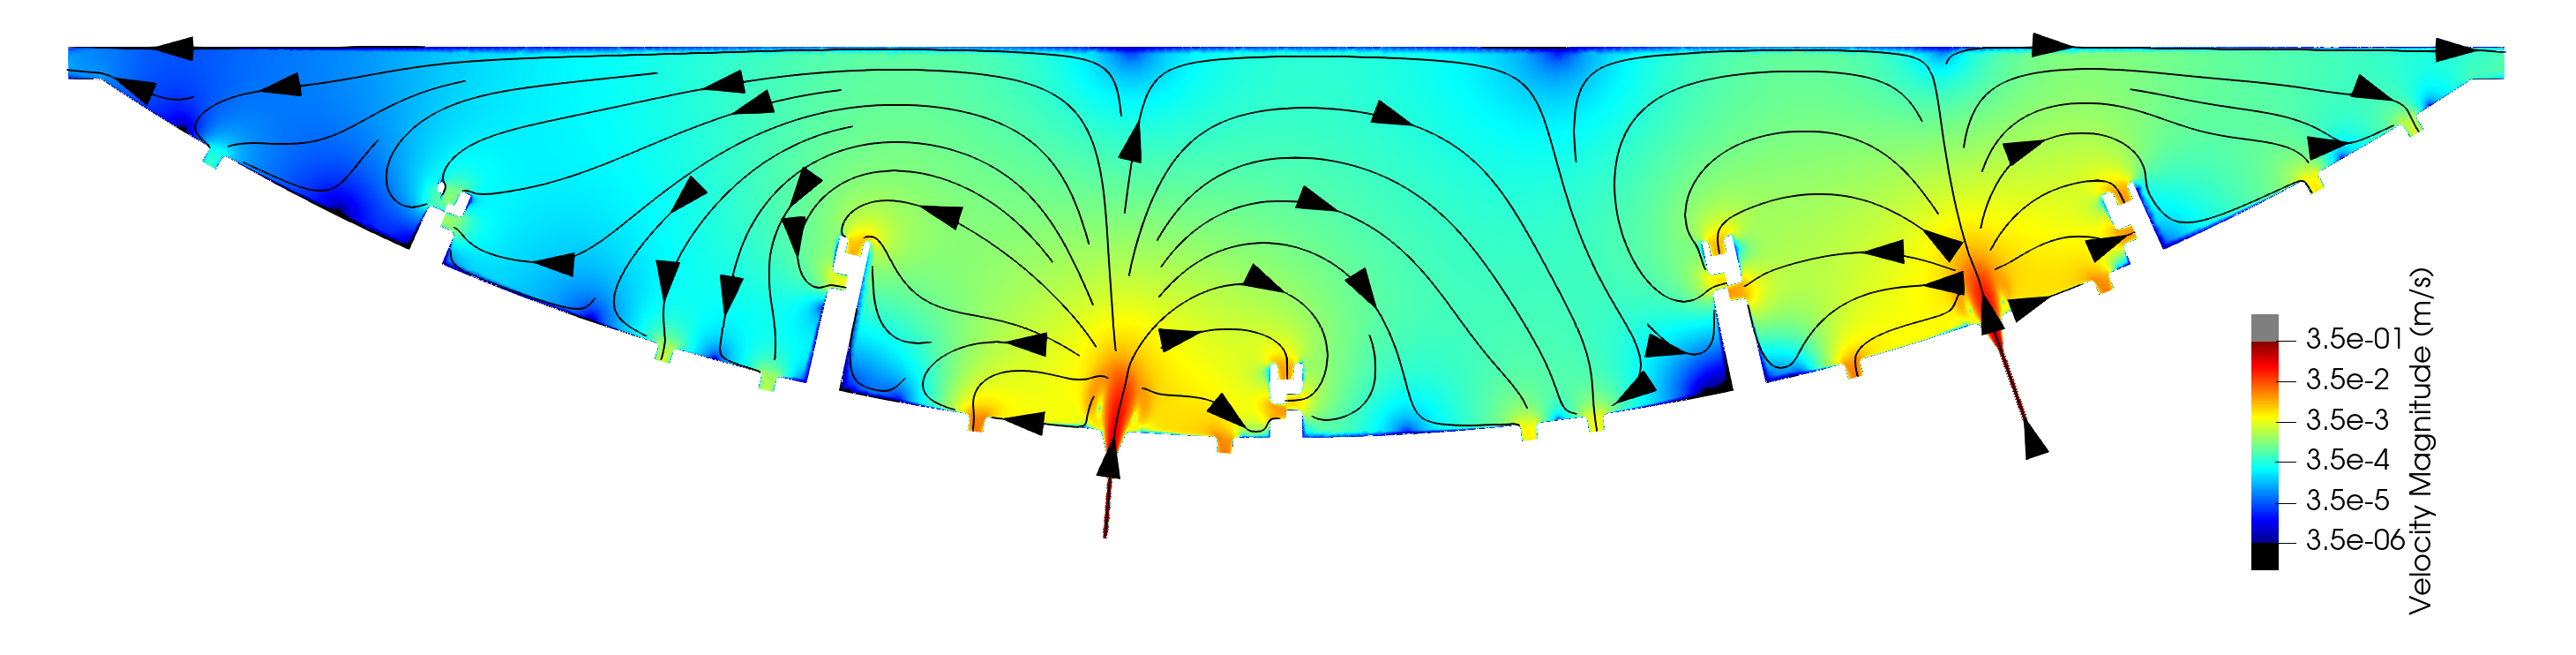
\includegraphics[width=181.5pt,height=46.12pt]{diagrams/results-variations/444-velocity.png}};
%Image [id:dp17912691189229846] 
\draw (461.51,98.25) node  {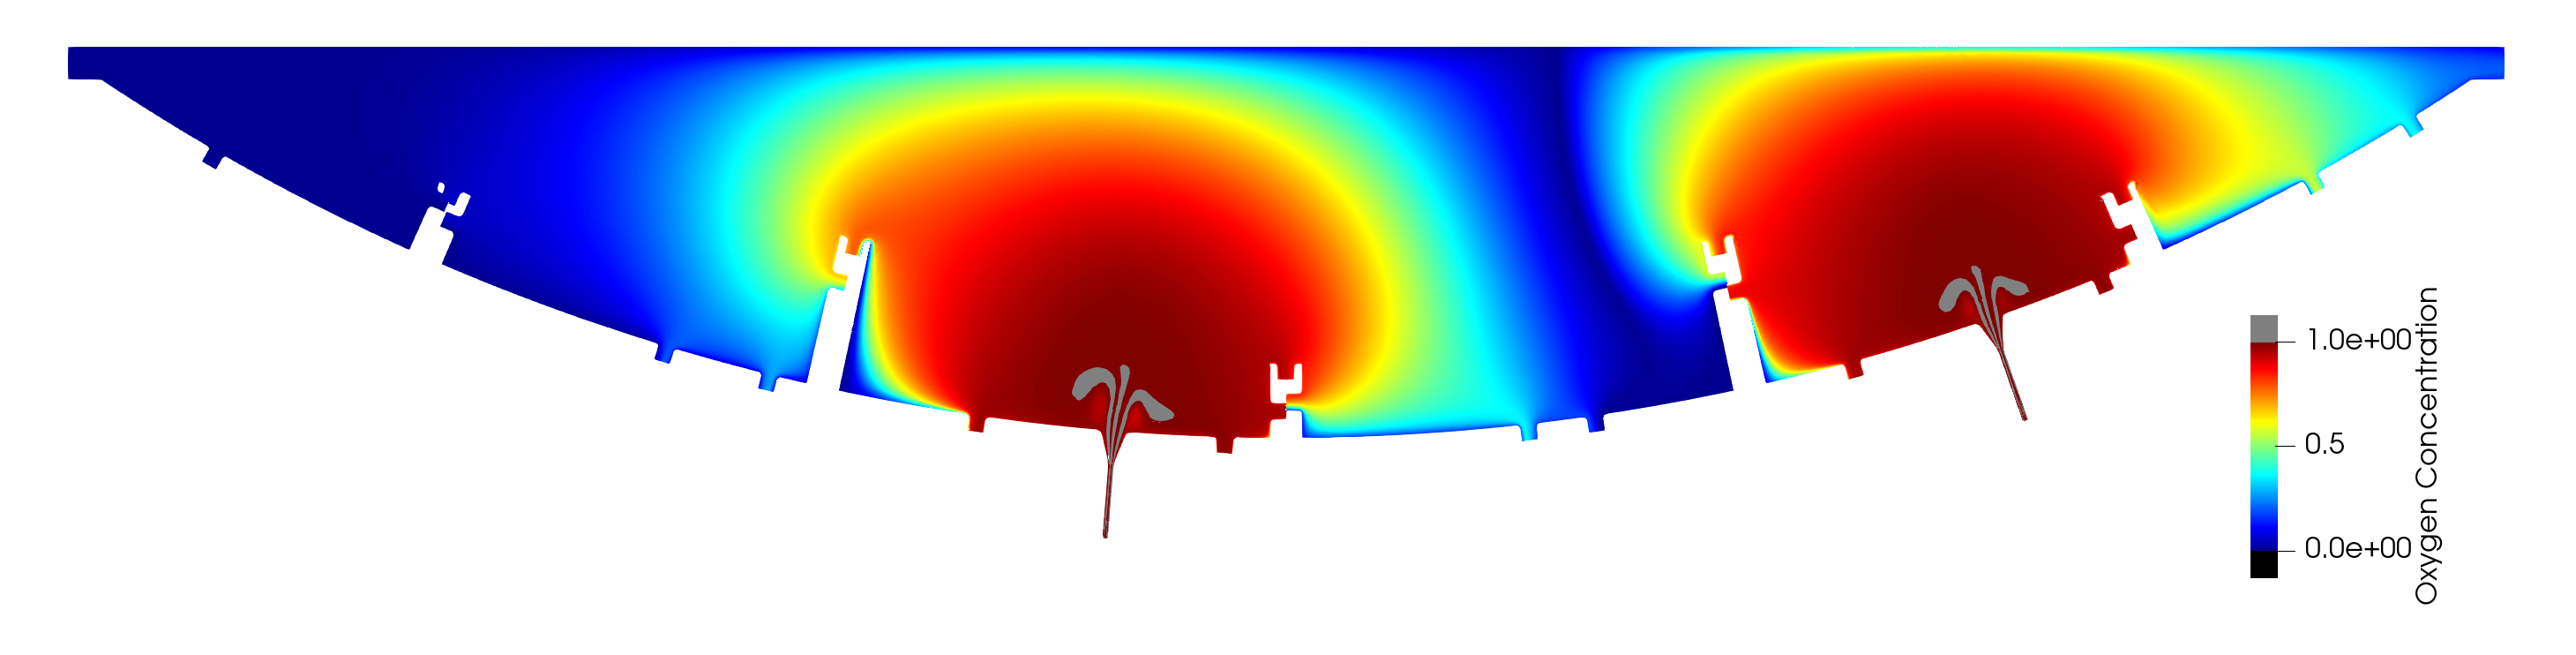
\includegraphics[width=181.52pt,height=46.13pt]{diagrams/results-variations/444-oxygen.png}};
%Image [id:dp7793537016904728] 
\draw (136,169.75) node  {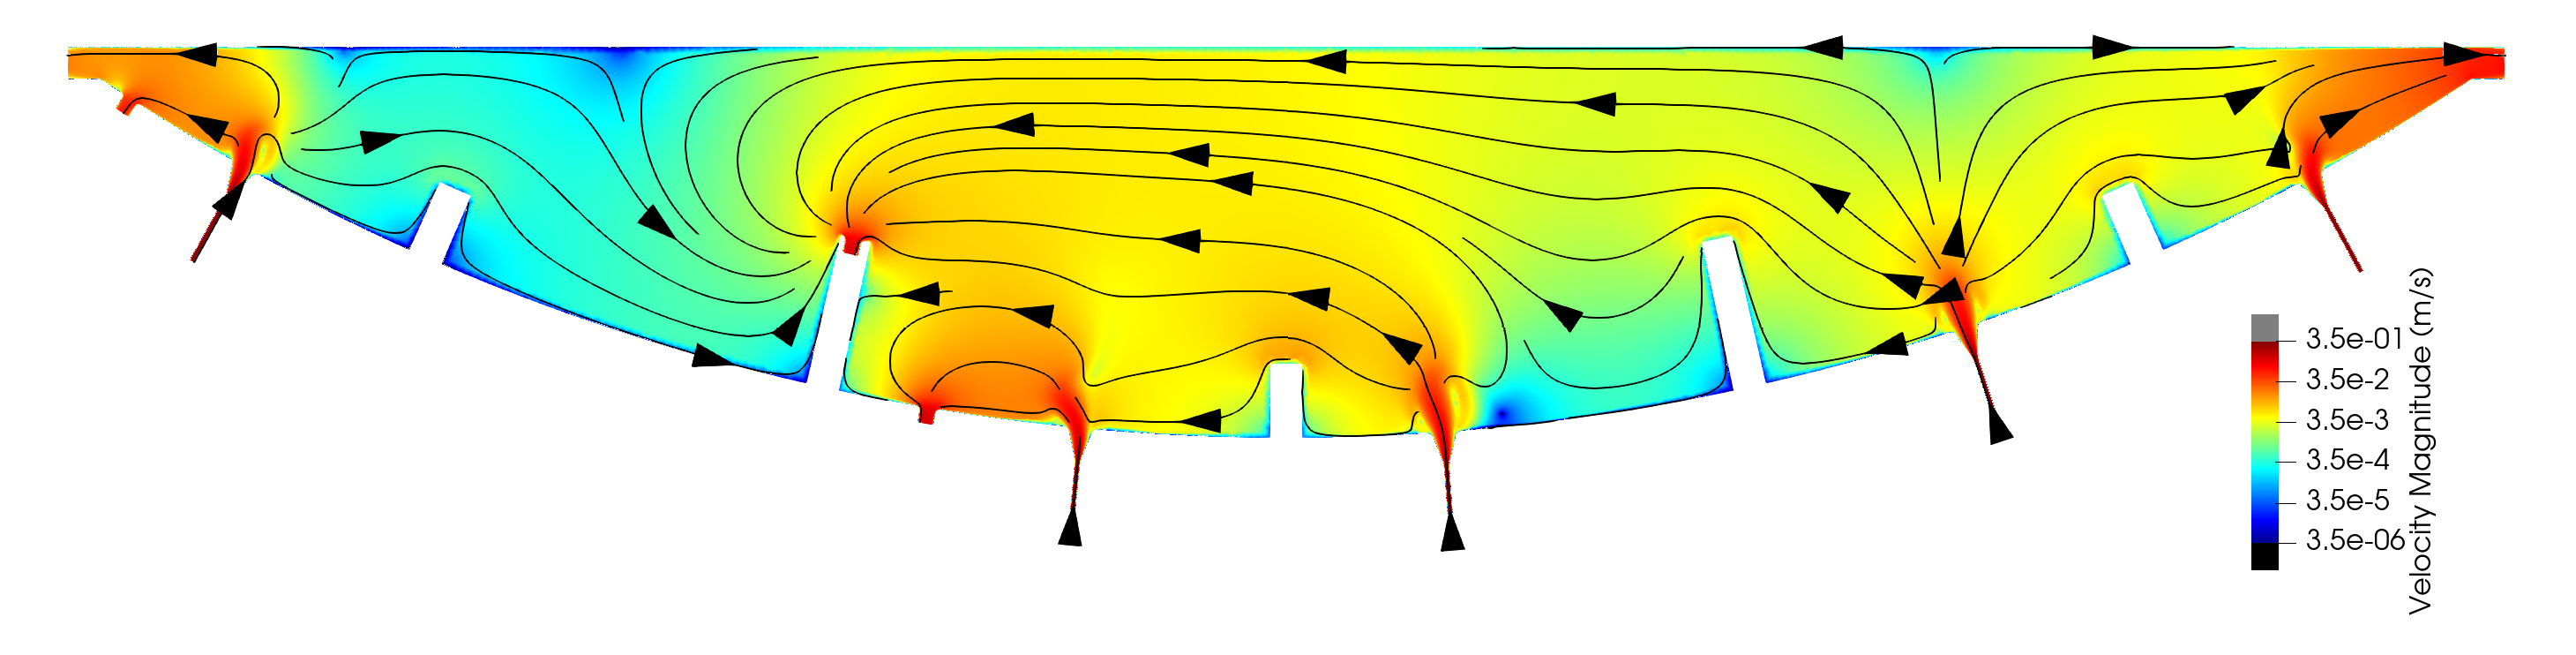
\includegraphics[width=181.5pt,height=46.12pt]{diagrams/results-variations/122-velocity.png}};
%Image [id:dp12012060465786312] 
\draw (135.51,224.75) node  {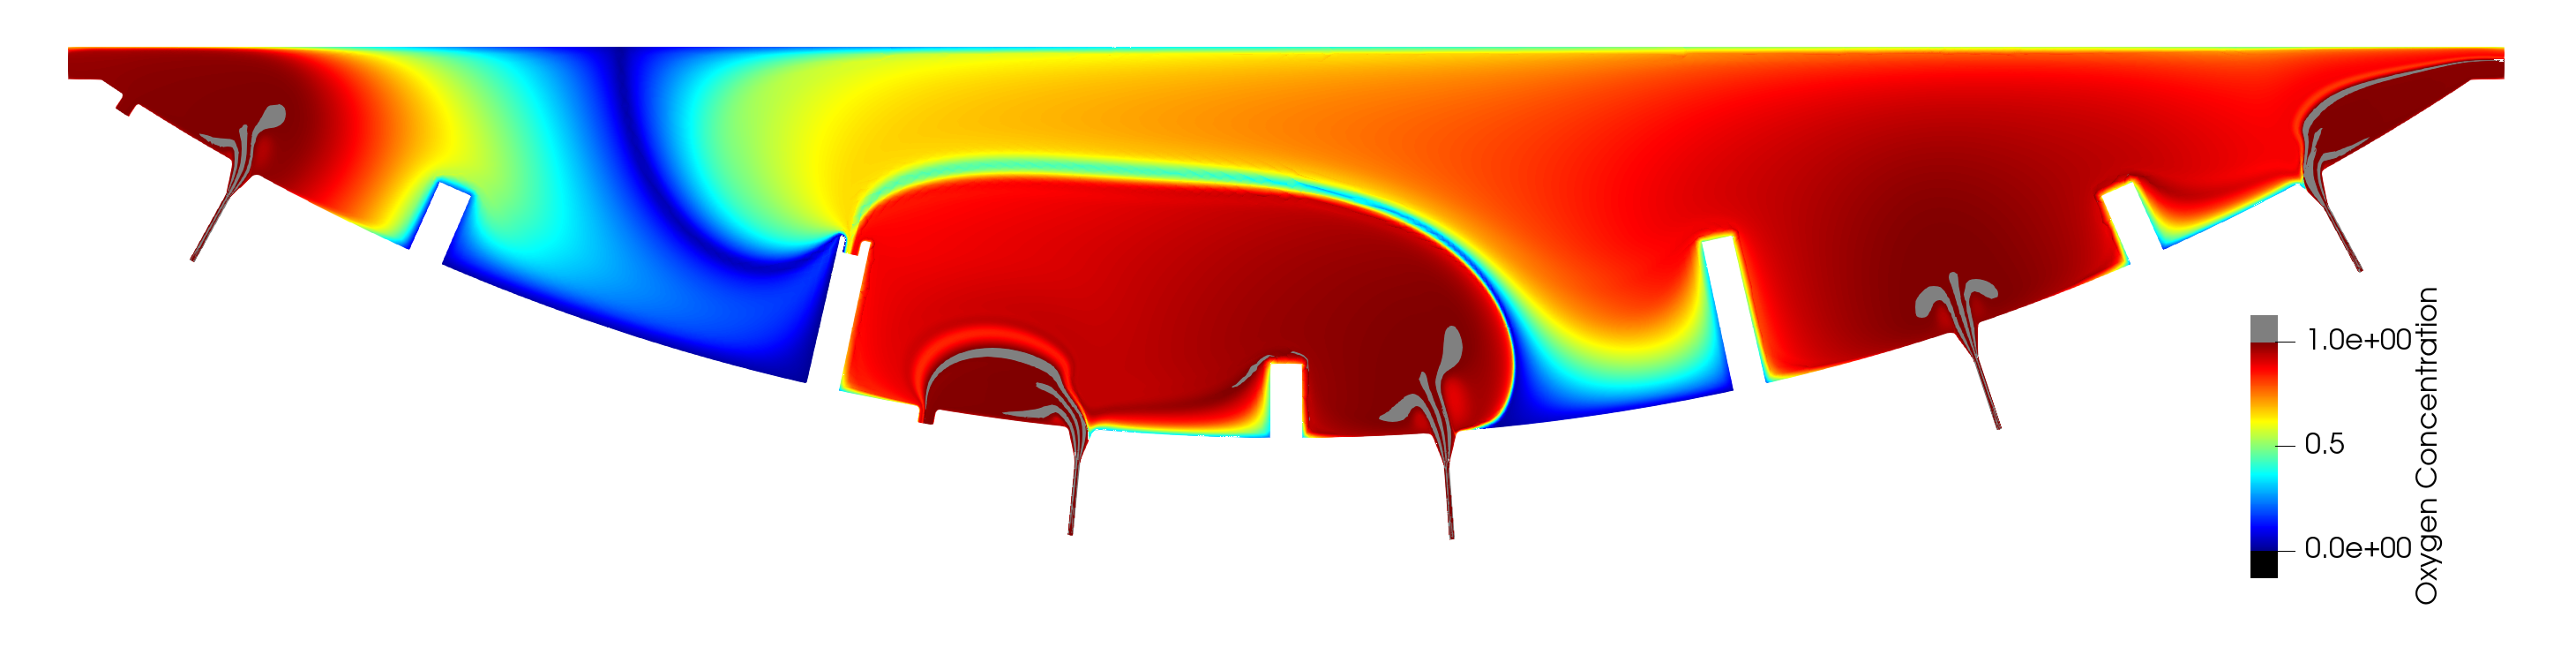
\includegraphics[width=181.52pt,height=46.13pt]{diagrams/results-variations/122-oxygen.png}};
%Image [id:dp8850565235206664] 
\draw (462.5,169.25) node  {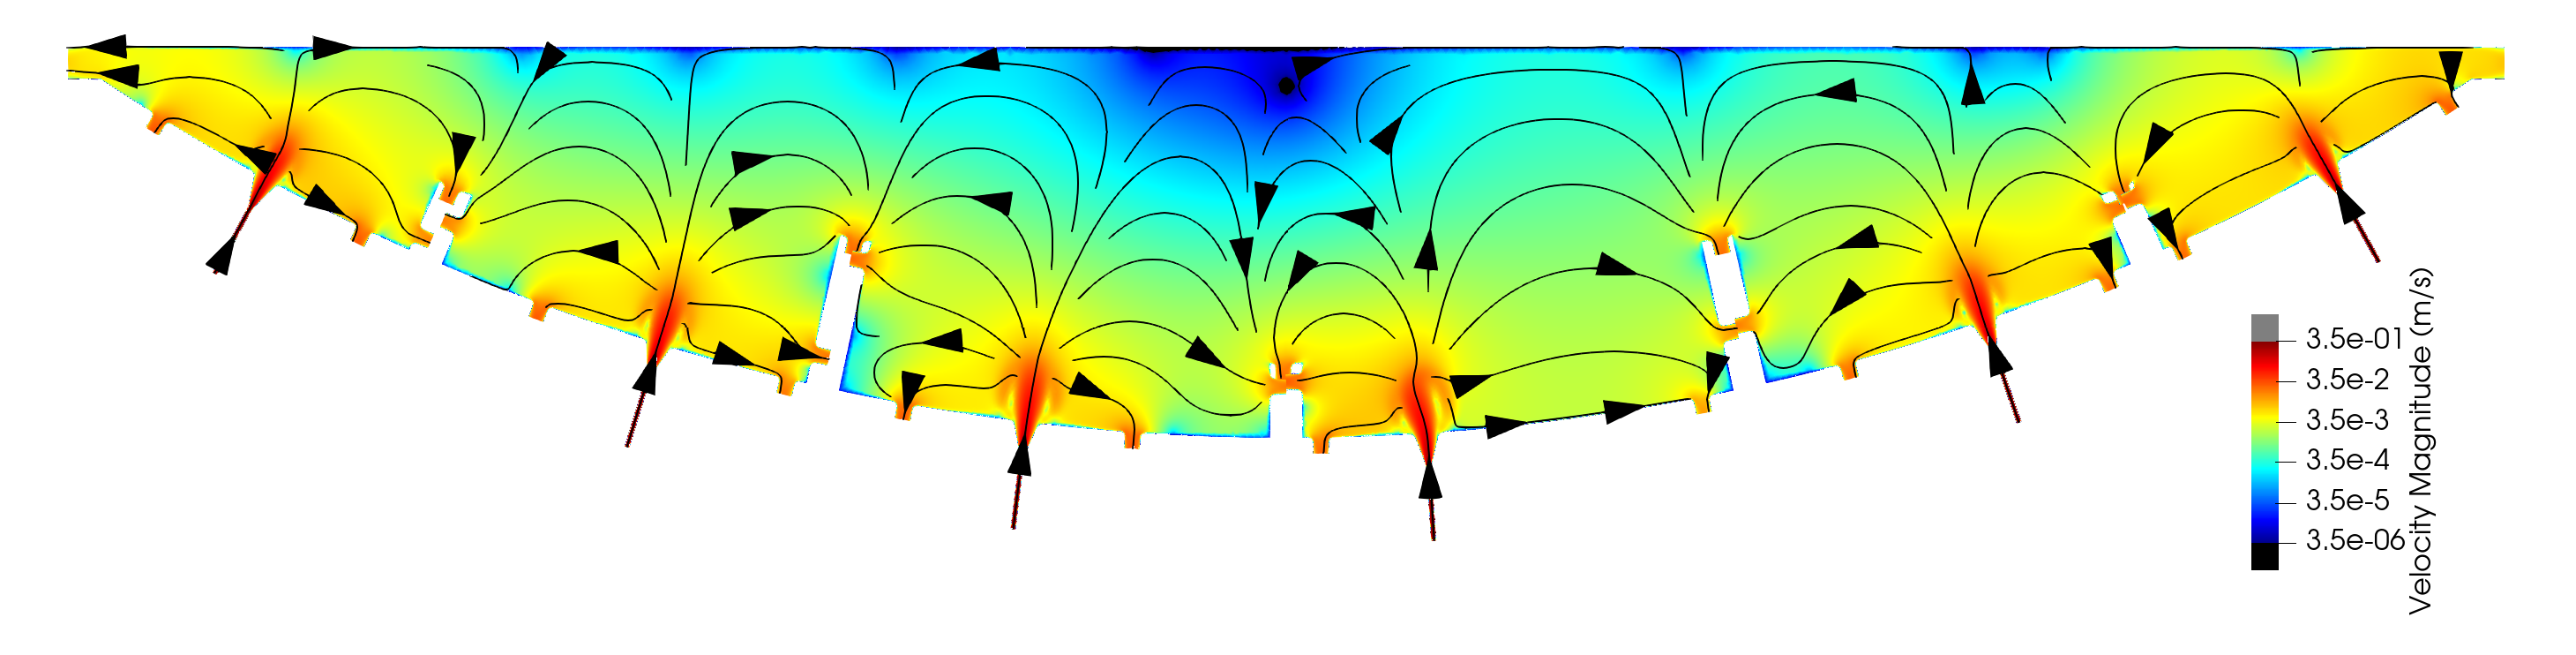
\includegraphics[width=181.5pt,height=46.12pt]{diagrams/results-variations/90-velocity.png}};
%Image [id:dp16362593587874552] 
\draw (462.01,224.25) node  {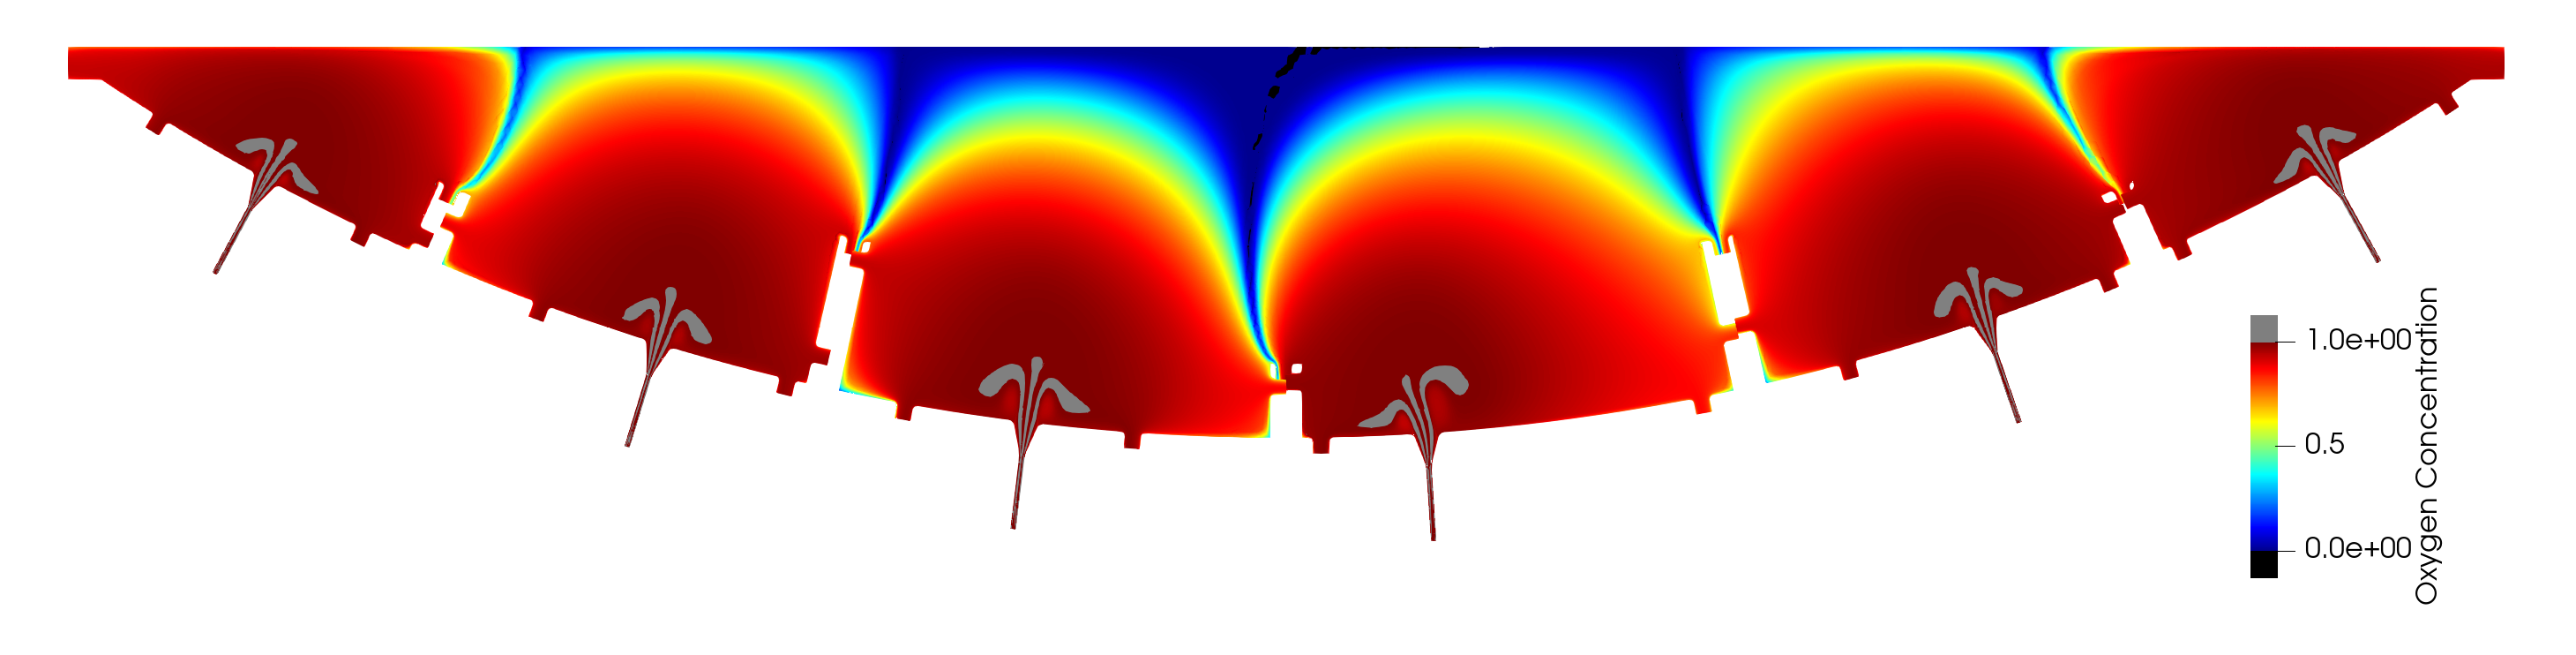
\includegraphics[width=181.52pt,height=46.13pt]{diagrams/results-variations/90-oxygen.png}};

% Text Node
\draw (258.42,70.43) node [anchor=west] [inner sep=0.75pt]    {$ \begin{array}{l}
N_{\text{A}} =1\\
N_{\text{V}} =1
\end{array}$};
% Text Node
\draw (584.92,69.93) node [anchor=west] [inner sep=0.75pt]    {$ \begin{array}{l}
N_{\text{A}} =2\\
N_{\text{V}} =24
\end{array}$};
% Text Node
\draw (258.92,196.43) node [anchor=west] [inner sep=0.75pt]    {$ \begin{array}{l}
N_{\text{A}} =5\\
N_{\text{V}} =3
\end{array}$};
% Text Node
\draw (585.42,195.93) node [anchor=west] [inner sep=0.75pt]    {$ \begin{array}{l}
N_{\text{A}} =6\\
N_{\text{V}} =27
\end{array}$};


\end{tikzpicture}

                    \caption{}
                    \label{fig:mega-vessels1:simulations}
                \end{subfigure}
                \caption{(a) Graphs that show how $\bar{v}(\Omega_\text{IVS})$ and $\bar{c}$ vary according to the number of vessels. From left to right, each column has grouped the data from all $N_\text{sim}$ simulations according to $N_\text{A}$, $N_\text{V}$, and $N_\text{V}/N_\text{A}$. In each panel, the blue dotted line corresponds to the median, and the surrounding blue shaded region corresponds to the area between the $25$th and $75$th percentile of the data. Individual outlier points are plotted outside this region. Orange lines visualise a subset of the data, as indicated by the inset legends. (b) Four selected simulations out of $N_\text{sim}$, visualising the velocity field (top) and the oxygen concentration field (bottom); the numbers of arteries $N_\text{A}$ and veins $N_\text{V}$ are indicated. The coloured crosses in (a) correspond to the coloured boxes surrounding the simulations in (b). The colour scales are small in subfigure (b), but range as before: $|\vec{u}| \in [3.5\times10^{-6}, 3.5\times10^{-1}]$ and $c \in [0, 1]$.}
                \label{fig:mega-vessels1}
            \end{figure}
        
            Upon studying Figure \ref{fig:mega-vessels1:results}, we firstly note that the coloured crosses (indicating the four chosen realisations) sometimes fall outside the shaded areas; these particular simulations were chosen to demonstrate the relatively high variability in the data presented here. Secondly, there are some clear correlations between the number of arteries and both $\bar{v}(\Omega_\text{IVS})$ and $\bar{c}$; according to the results presented here, placentas with $N_\text{A} = 6$ maximise both the average speed of the blood flow and the uptake of oxygen. Conversely, the maximal values of $\bar{v}(\Omega_\text{IVS})$ for the number of veins is when $N_\text{V} = 0$, which is because marginal sinuses are always available here as a route of venous drainage and will draw the blood flow across the domain.
            
            As can be seen in the corresponding four visualisations of the velocity fields in Figure \ref{fig:mega-vessels1:simulations}, the flow is, in general, much slower when $N_\text{V}$ is higher; this is because, when there are more veins, fluid has the opportunity to `short-circuit' and exit through nearby veins, rather than be drawn across the placenta. This is illustrated when comparing the red- and green-boxed simulations in Figure \ref{fig:mega-vessels1:simulations}, where in the former the fluid speed is at least an order of magnitude slower than the latter in many parts of the domain. The maximal values of $\bar{c}$ are again when $N_\text{A} = 6$ or $N_\text{V} = 0$, but the effect of the veins is less powerful here. Instead, it is the number of arteries that has the greatest effect on $\bar{c}$, although there is a clear plateau as $N_\text{A}$ approaches $6$; this is further shown in the second column, where the variability for varying $N_\text{V}$ is very large, which is due to the number of arteries in each simulation dominating in the value of $\bar{c}$. Interestingly, for $N_\text{V}/N_\text{A}$, there is a much less variable relationship for both $\bar{v}(\Omega_\text{IVS})$ and $\bar{c}$, shown by the smaller shaded region surrounding the dotted median line, showing that this ratio is important in determining $\bar{v}(\Omega_\text{IVS})$ and $\bar{c}$ for a given simulation. The maximal values for both $\bar{v}$ and $\bar{c}$ are obtained when $N_\text{V}/N_\text{A} = 0$.
            
            The orange lines plot a subset of the data so that we can more clearly see the effects of varying $N_\text{A}$ and $N_\text{V}$ separately. The values of $\bar{v}(\Omega_\text{IVS})$ and $\bar{c}$ for varying $N_\text{A}$ and fixed $N_\text{V} = 27$ in the first column are plotted in orange and are clearly less variable than when any $N_\text{V}$ is considered in blue, and shows that having more veins overall decreases both $\bar{v}(\Omega_\text{IVS})$ and $\bar{c}$; this supports the idea that more veins may lead to more short-circuiting behaviour and oxygen leaving the placenta in relatively high concentration \cite{erianMaternalPlacentalBlood1977,chernyavskyMathematicalModelIntervillous2010}. Indeed, this is also the case when considering the second column, where $N_\text{V}$ is varied. Fixing now $N_\text{A} = 6$ and considering variations in $N_\text{V}$ shown in orange in the second column, we see that high numbers of arteries overall increases $\bar{v}(\Omega_\text{IVS})$ and $\bar{c}$, which is sensible when considering the increased flux of blood and oxygen entering the placenta.

            Existing MRI studies have measured the mean flow speed in vivo to be between $\qty{0.4}{\milli\metre\per\second}$ and $\qty{0.94}{\milli\metre\per\second}$ \cite{lecarpentierComputationalFluidDynamic2016,dellschaftHaemodynamicsHumanPlacenta2020,serovOptimalVilliDensity2015}; this range corresponds to the data shown for $N_\text{A} = 1$ and $N_\text{A} = 2$, but $\bar{v}(\Omega_\text{IVS})$ is in general higher for other numbers of vessels. The faster mean speeds measured in our simulations could be due to the study of 2D flow in this thesis, or because a large number of arteries in this setting is unphysical. Furthermore, the MRI study by \citeauthor{dellschaftHaemodynamicsHumanPlacenta2020} \cite{dellschaftHaemodynamicsHumanPlacenta2020} found that diseased placentas in general had a faster mean speed of $\qty{0.7}{\milli\metre\per\second}$, as opposed to $\qty{0.4}{\milli\metre\per\second}$ for healthy placentas. From this, our results suggest that placentas with a large number of arteries or small number of veins may be characteristic of placental disease; however, an interesting contradiction arises here, as these are the cases where oxygen uptake is maximised in our results, which in itself suggests that these are the best-performing placentas.

            In summary, these results show that increasing $N_\text{A}$ increases both $\bar{v}(\Omega_\text{IVS})$ and $\bar{c}$, with the effect most pronounced for $\bar{c}$, and reducing $N_\text{V}$ increases both $\bar{v}(\Omega_\text{IVS})$ and $\bar{c}$, with the effect most pronounced for $\bar{v}(\Omega_\text{IVS})$. Plotting $\bar{v}(\Omega_\text{IVS})$ and $\bar{c}$ against the ratio $N_\text{V}/N_\text{A}$ gave a smaller interquartile range, and overall for higher $N_\text{V}/N_\text{A}$ gave decreasing values of the two measures.

        \subsection{Effects on \texorpdfstring{$v_\text{slow}$}{slow velocity percentage}} \label{sec:nutrient-uptake:slow-velocity-percentage}
            For a given simulation, we define four velocity thresholds under which to define `slow velocity':
            \begin{itemize}
                \item $V_\text{threshold} = \bar{v}(\Omega_\text{IVS})~\unit{\metre\per\second}$: average speed of this simulation over $\Omega_\text{IVS}$. 
                \item $V_\text{threshold} = \bar{v}(\Omega)~\unit{\metre\per\second}$: average speed of this simulation over $\Omega$.
                \item $V_\text{threshold} = \qty{0.0005}{\metre\per\second}$: threshold taken by definition of slow velocity in \citeauthor{dellschaftHaemodynamicsHumanPlacenta2020} \cite{dellschaftHaemodynamicsHumanPlacenta2020}.
                \item $V_\text{threshold} = \qty{0.0026}{\metre\per\second}$: threshold equals $\bar{v}(\Omega)$ calculated from the placenta simulation in \S\ref{sec:numerical-methods:blood-flow-experiments:comparison}.
            \end{itemize}
            We emphasise that the first two of these thresholds relate to the average speed of the given simulation, whereas the last two of these choices are fixed across all simulations. 
            
            We chose the threshold $V_\text{threshold} = \qty{0.0005}{\metre\per\second}$ as it has been previously categorised as a threshold for `slow flow' in the literature; \citeauthor{dellschaftHaemodynamicsHumanPlacenta2020} \cite{dellschaftHaemodynamicsHumanPlacenta2020} found that MRI scans of the placenta contained regularly spaced regions of relatively fast-moving blood ($|\vec{u}| > \qty{0.001}{\metre\per\second}$) interspersed with regions of slow-moving blood ($|\vec{u}| < \qty{0.0005}{\metre\per\second}$); they were able to identify regions of fast-moving blood to be close to spiral arteries, with the slow regions likely occurring in the surrounding IVS. 

            The final choice of threshold, $V_\text{threshold} = \qty{0.0026}{\metre\per\second}$, was chosen by computing $\bar{v}(\Omega)$ on the symmetric placenta simulation of NSD presented in \S\ref{sec:numerical-methods:blood-flow-experiments:comparison}. We chose to compare against this simulation because of its similarity to the position and number of vessels that have previously been used in the mathematical modelling literature \cite{lecarpentierComputationalFluidDynamic2016,chernyavskyMathematicalModelIntervillous2010}.

            Inspecting Figure \ref{fig:mega-vessels2}, these first two thresholds show that, regardless of the number and positions of vessels, the percentage of flow slower than the average speed remains roughly constant at approximately $30\%$; this is not immediately obvious by the flow simulations we've investigated so far.

            \begin{figure}
                \centering
                % Date generated: 2024-05-18 17:35:33
                % Commit: eac341b1ef691c92e8badeb0786f784648653b40
                % File run: ./drivers/variations_2024-03-21/vary_mega-vessels.py
                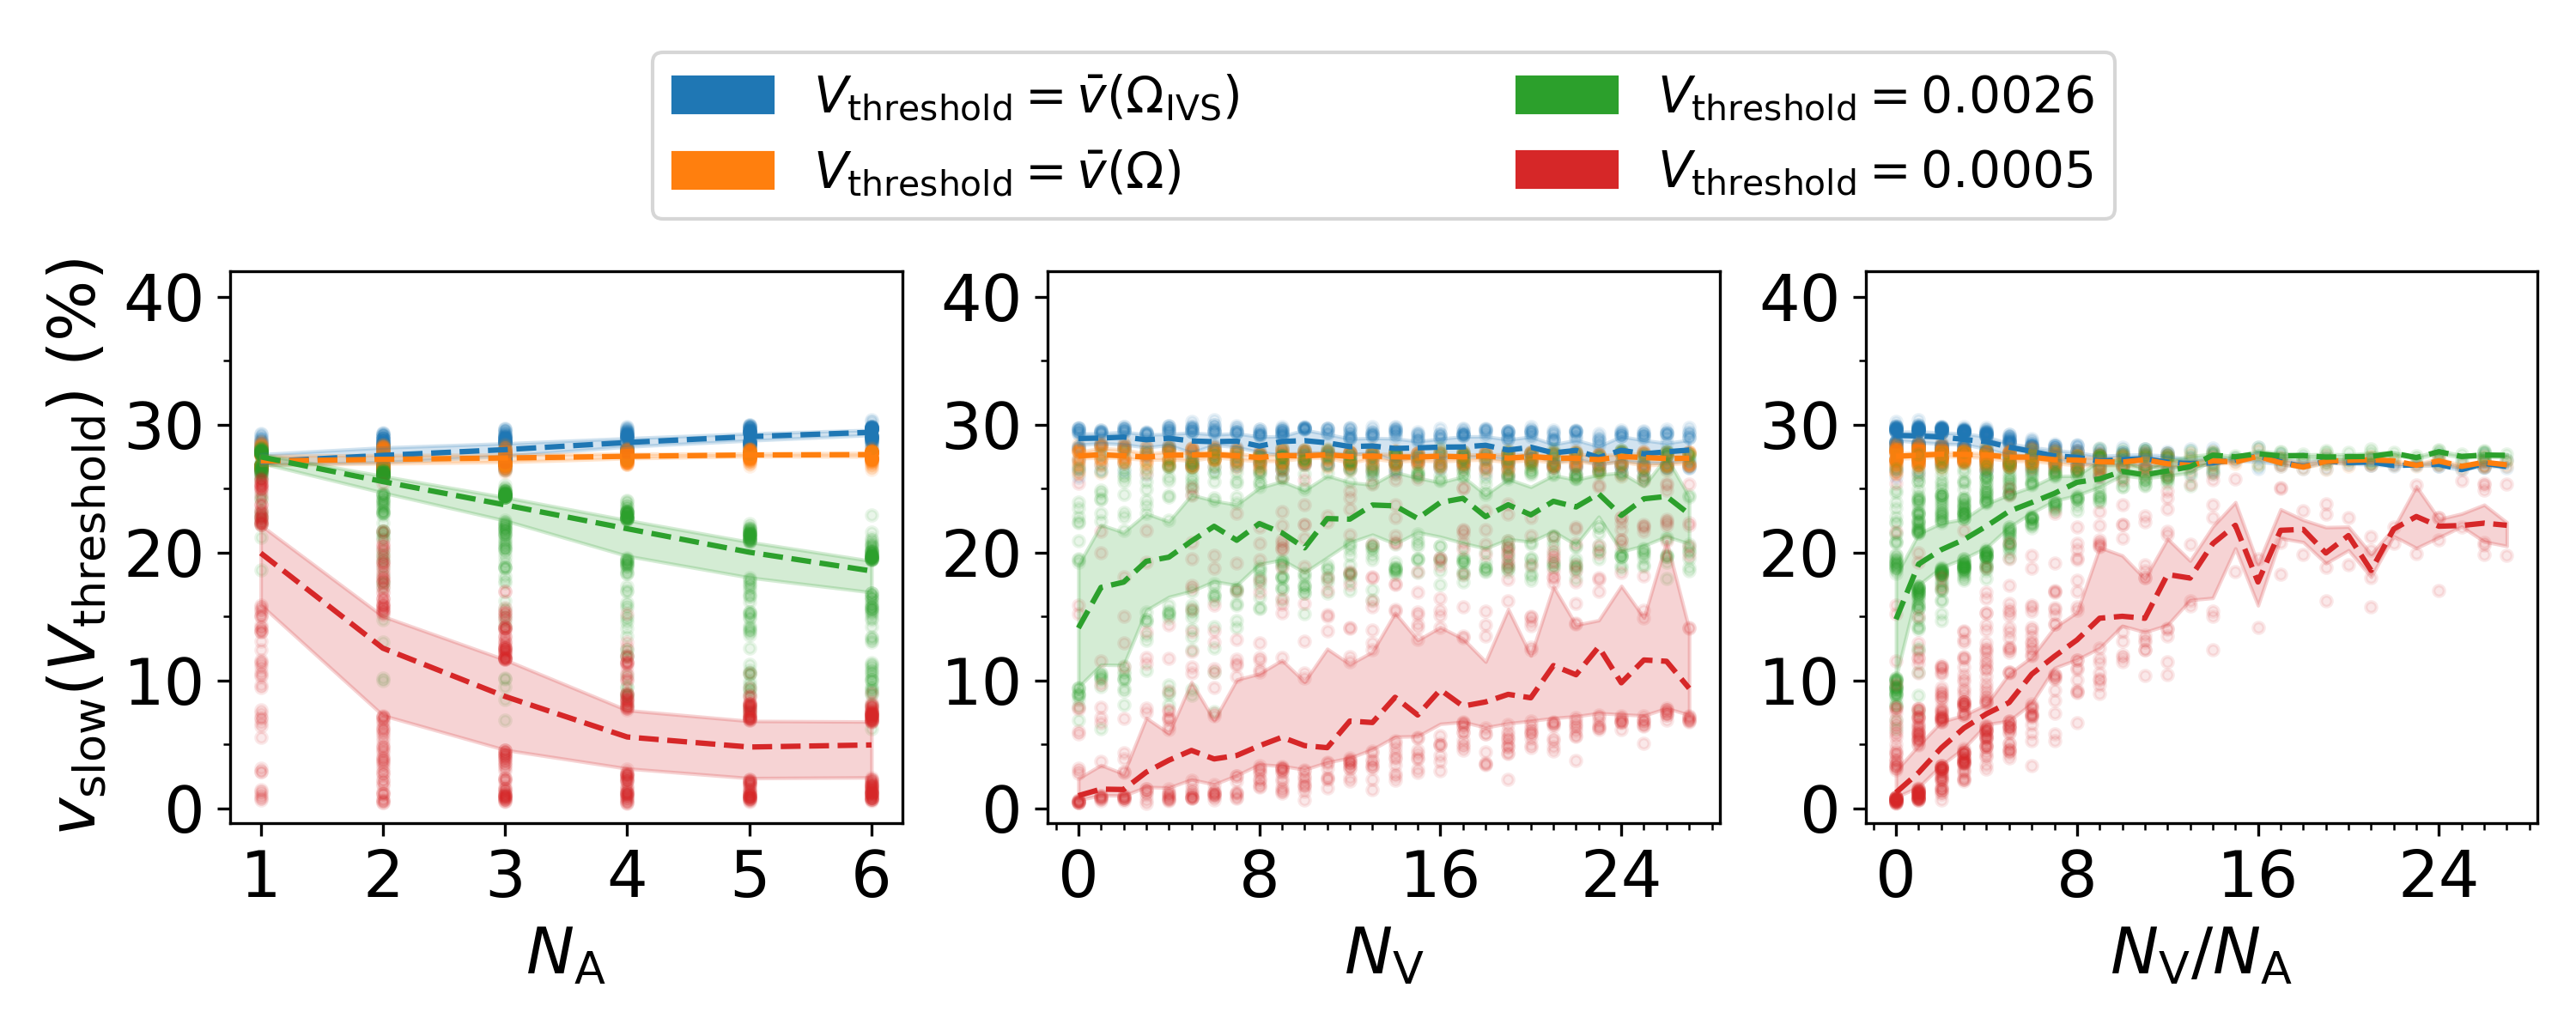
\includegraphics[width=\textwidth]{diagrams/results-variations/mega2_no-arteries_no-veins_veins-to-arteries.png}
                \caption{Graphs that show how $v_\text{slow}$ varies with changes in the number of arteries and veins. The first column plots these measures for varying the number of arteries from $1$ to $6$, the second column plots these measures for varying the number of veins from $0$ to $27$, and the third column plots these measures for the ratio between the number of veins and the number of arteries. In each panel, the dotted lines correspond to the median, and the surrounding shaded regions correspond to the area between the $25$th and $75$th percentile of the data, with individual outlier points plotted outside these regions. The legend above the plots indicates the choice of $V_\text{threshold}$.}
                \label{fig:mega-vessels2}
            \end{figure}
            
            There is, however, a slight separation between $v_\text{slow}(V_\text{threshold})$ for $V_\text{threshold} = \qty{0.0005}{\metre\per\second}$ and $\qty{0.0026}{\metre\per\second}$, with the former decreasing more rapidly with increasing $N_\text{A}$. Although there is a separation in these values of $v_\text{slow}$, the overall trends are the same, with $v_\text{slow}$ decreasing for larger $N_\text{A}$ and increasing for larger $N_\text{V}$; these results in general agree with those presented in \S\ref{sec:nutrient-uptake:average-velocity-and-concentration}. \citeauthor{dellschaftHaemodynamicsHumanPlacenta2020} \cite{dellschaftHaemodynamicsHumanPlacenta2020} found that diseased PE placentas generally had a lower proportion of slow-moving flow than healthy placentas; from the results presented here, this could suggest that placentas with either a small number of arteries or a large number of veins could be characteristic of PE placentas. However, a disparity arises here, as MRI scan slices of healthy placentas gave approximately $57\%$ of slow-moving blood below this threshold \cite{dellschaftHaemodynamicsHumanPlacenta2020}, which is much higher than any of the values presented here. As previously suggested, this could be due to the 2D study of flow here.

        \subsection{Effects on venous drainage}
            We now investigate the exit routes by the blood and the oxygen by considering $v_\text{flux}$ and $c_\text{flux}$ for basal plate, septal wall, and marginal sinus veins. For those results presented in Figure \ref{fig:mega-vessels3}, we compute
            \begin{equation*}
                \frac{v_\text{flux}(S)}{v_\text{flux}(\Gamma_\text{in})}
            \end{equation*}
            and
            \begin{equation*}
                \frac{c_\text{flux}(S)}{c_\text{flux}(\Gamma_\text{in})}
            \end{equation*}
            for three different choices of $S$: namely, we take these to be $S \subseteq \Gamma_\text{out}$ according to whether veins are placed on the basal plate ($\Gamma_\text{out,bp}$), septal wall ($\Gamma_\text{out,sw}$), or marginal sinus ($\Gamma_\text{out,ms}$).

            \begin{figure}
                \centering
                % Date generated: 2024-05-18 17:35:33
                % Commit: eac341b1ef691c92e8badeb0786f784648653b40
                % File run: ./drivers/variations_2024-03-21/vary_mega-vessels.py
                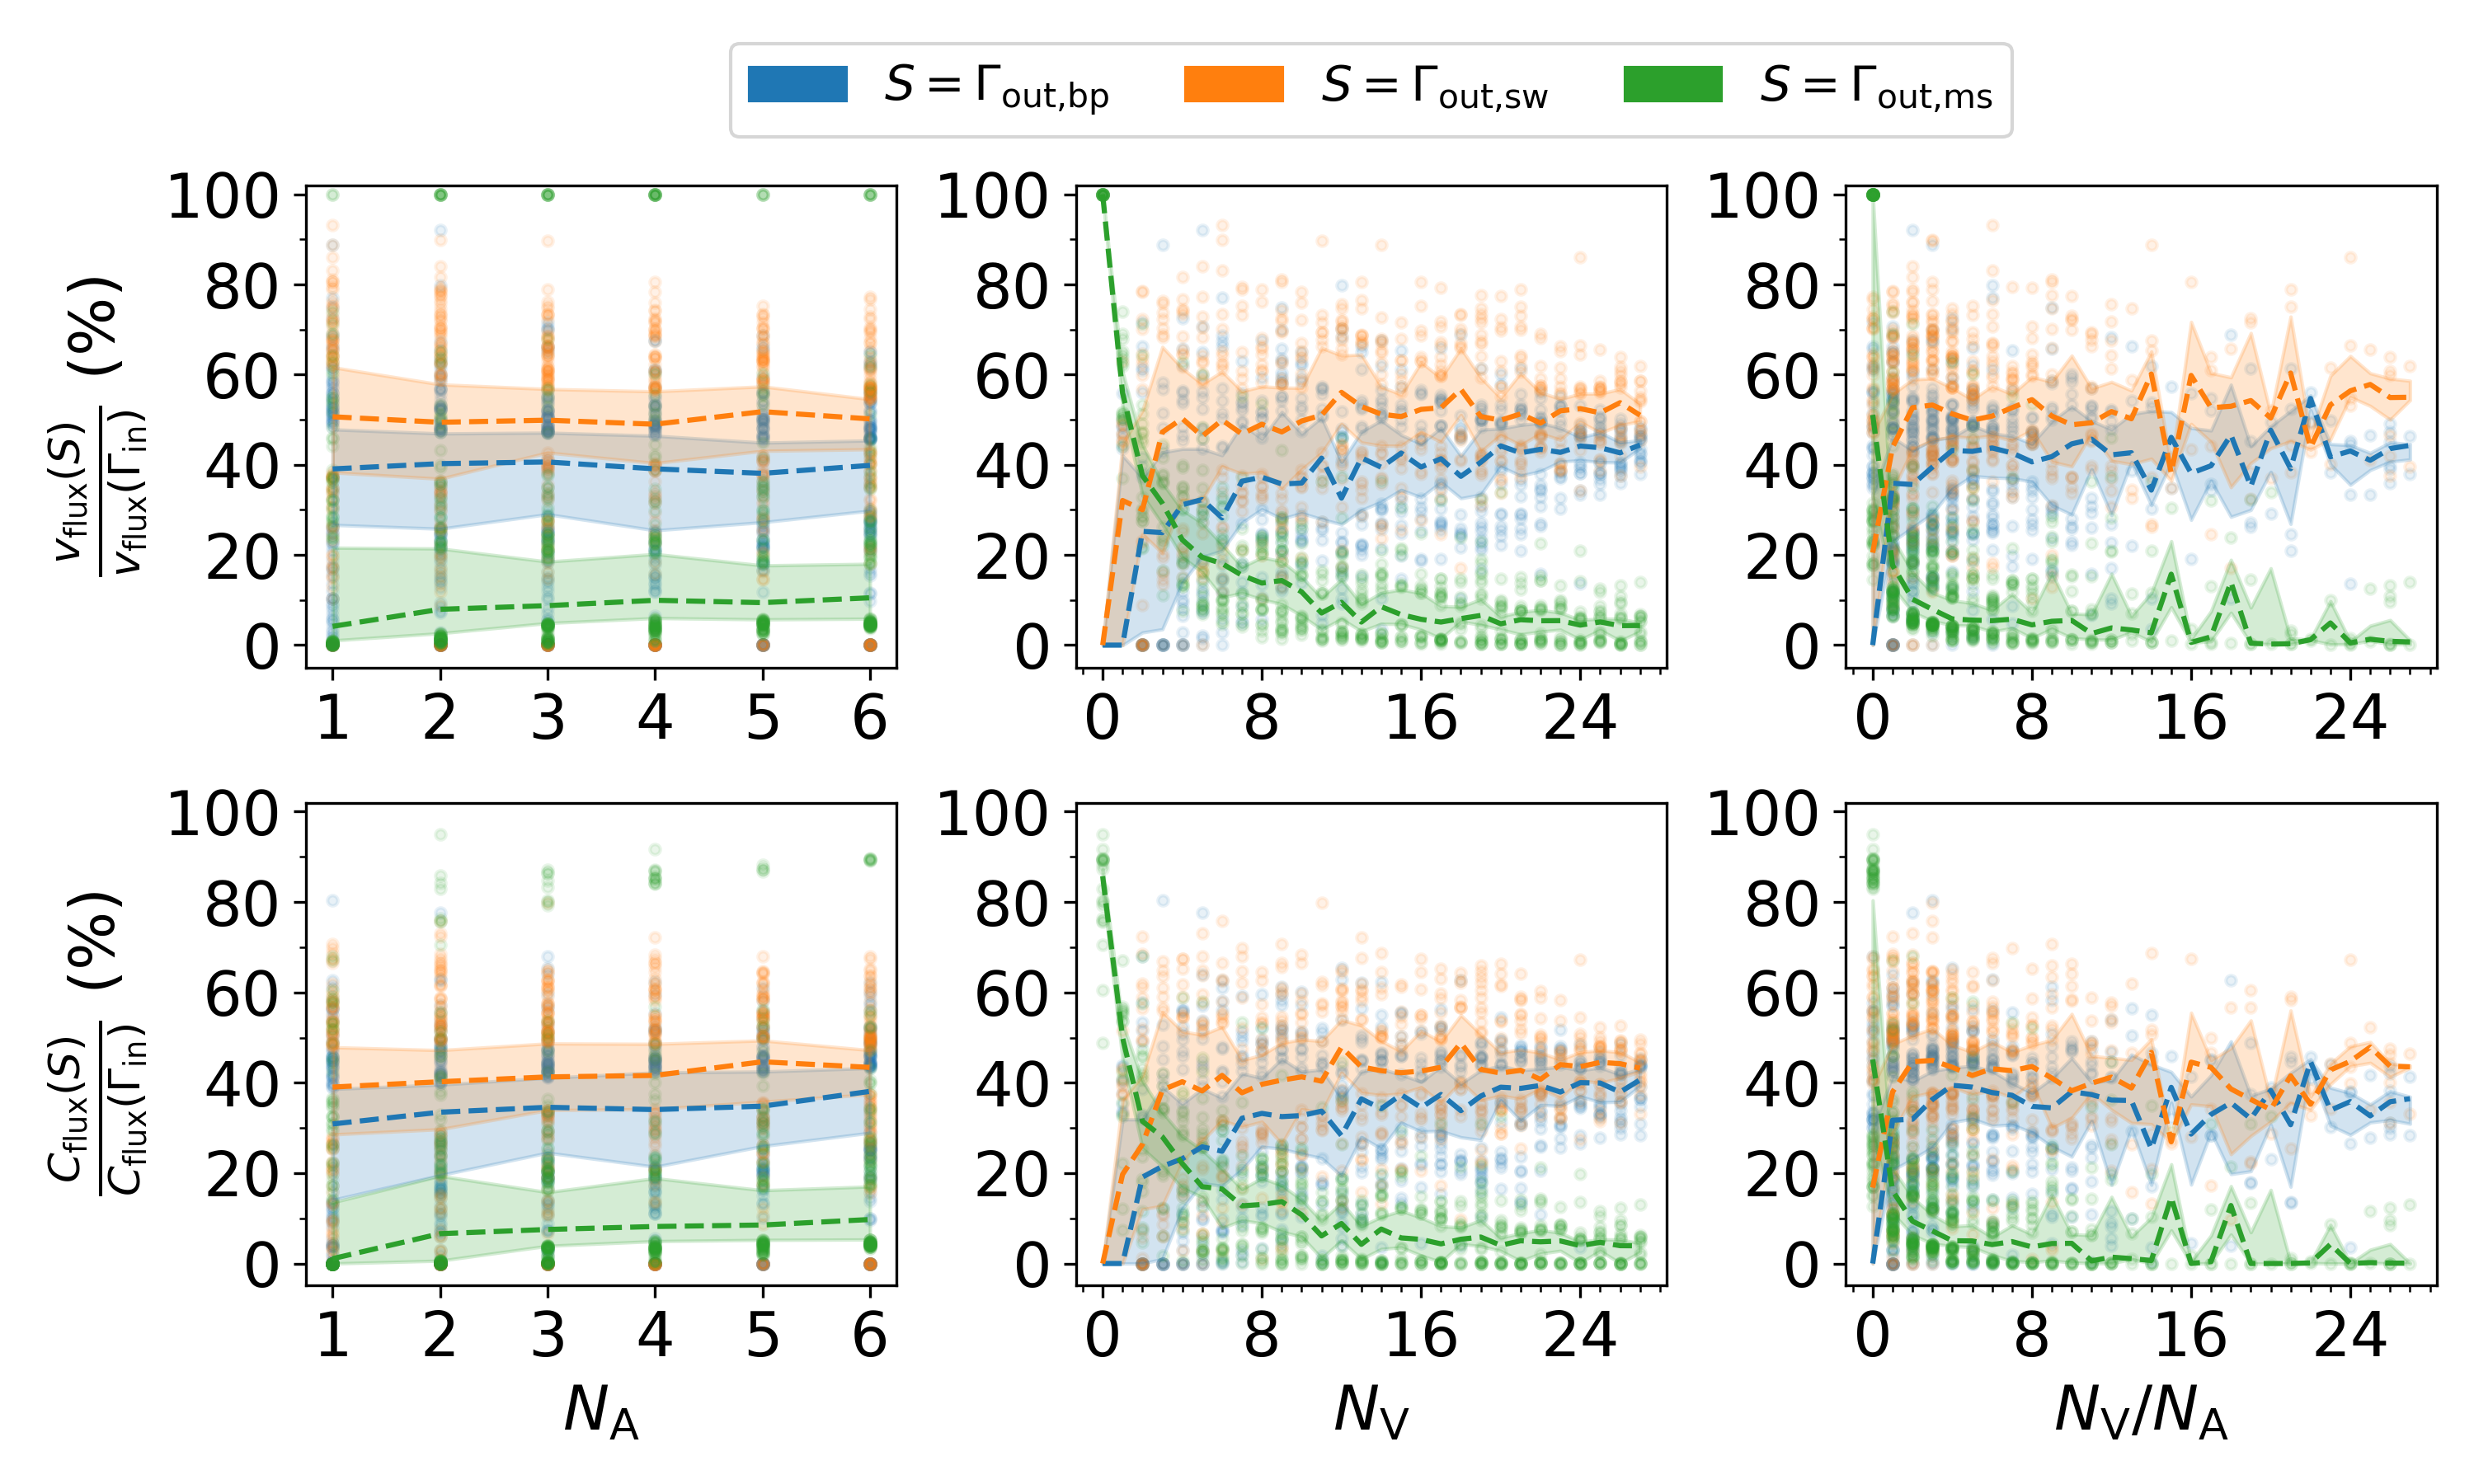
\includegraphics[width=\textwidth]{diagrams/results-variations/mega3_no-arteries_no-veins_veins-to-arteries.png}
                \caption{Graphs that show how $v_\text{flux}$ and $c_\text{flux}$ vary with changes in the number of arteries and veins. The first column plots these measures for varying the number of arteries from $1$ to $6$, the second column plots these measures for varying the number of veins from $0$ to $27$, and the third column plots these measures for the ratio between the number of veins and the number of arteries. In each panel, the dotted lines correspond to the median, and the surrounding shaded regions correspond to the area between the $25$th and $75$th percentile of the data, with individual outlier points plotted outside these regions. The legend above the plots indicates the choice of $S$.}
                \label{fig:mega-vessels3}
            \end{figure}
            
            We see little influence on route of exit for varying $N_\text{A}$. Instead, and unsurprisingly, the route of exit is strongly dependent upon the number of veins $N_\text{V}$. Fluid is conserved here, so we remark that
            \begin{equation*}
                \frac{v_\text{flux}(\Gamma_\text{out,bp})}{v_\text{flux}(\Gamma_\text{in})} + \frac{v_\text{flux}(\Gamma_\text{out,sw})}{v_\text{flux}(\Gamma_\text{in})} + \frac{v_\text{flux}(\Gamma_\text{out,ms})}{v_\text{flux}(\Gamma_\text{in})} = 1.
            \end{equation*}
            Therefore, as expected, we clearly see $100\%$ of the fluid exits through the marginal sinuses when $N_\text{V} = 0$.

            On the other hand, the oxygen flux exits the placenta at a lower concentration than how it entered, due to some of the oxygen being uptaken by the villous tree. For $N_\text{V} = 0$, approximately $85\%$ of the entering oxygen is exiting through the marginal sinus veins. Although not clearly illustrated here, calculating the sum of the blue, orange, and green curves (i.e., calculating $c_\text{flux}(\Gamma_\text{out})/c_\text{flux}(\Gamma_\text{in})$) gives values between $60\%$ and $90\%$ for all choices of numbers of vessels. This is a notably high concentration, considering that this is oxygen that could have been uptaken by the villous tree to be delivered to the fetus, which is arguably the placenta's most important function that we consider.
            
            As $N_\text{V}$ increases, the routes of exit for flow and oxygen slowly shift towards the basal plate and septal wall veins, for which there appears to be a slight preference for septal wall veins; however, this effect could be occurring simply because there are more septal wall veins through which blood can exit.

            We note that all three columns contain a relatively large amount of variability, especially in the third column for varying $N_\text{V}/N_\text{A}$; this suggests that $v_\text{flux}$ and $c_\text{flux}$ are more sensitive to something apart from the number of vessels, such as the position of the vessels. The third column shows more variability than the other two columns due to how $N_\text{A}$ and $N_\text{V}$ were sampled, meaning that there is a reduced number of simulations for higher numbers of $N_\text{V}/N_\text{A}$.

        \subsection{Effects on cross-placentone flow}
            We now discuss the effects on vessel variations on $v_\text{cross}$ in Figure \ref{fig:mega-vessels4}. This is an interesting feature to study because previous mathematical studies have mostly focussed on only single placentones \cite{lecarpentierComputationalFluidDynamic2016,chernyavskyMathematicalModelIntervillous2010}, whereas the study here focusses on a placenta with six placentones, which permits blood to move over the top of the septal walls.

            \begin{figure}
                \centering
                % Date generated: 2024-05-18 17:35:33
                % Commit: eac341b1ef691c92e8badeb0786f784648653b40
                % File run: ./drivers/variations_2024-03-21/vary_mega-vessels.py
                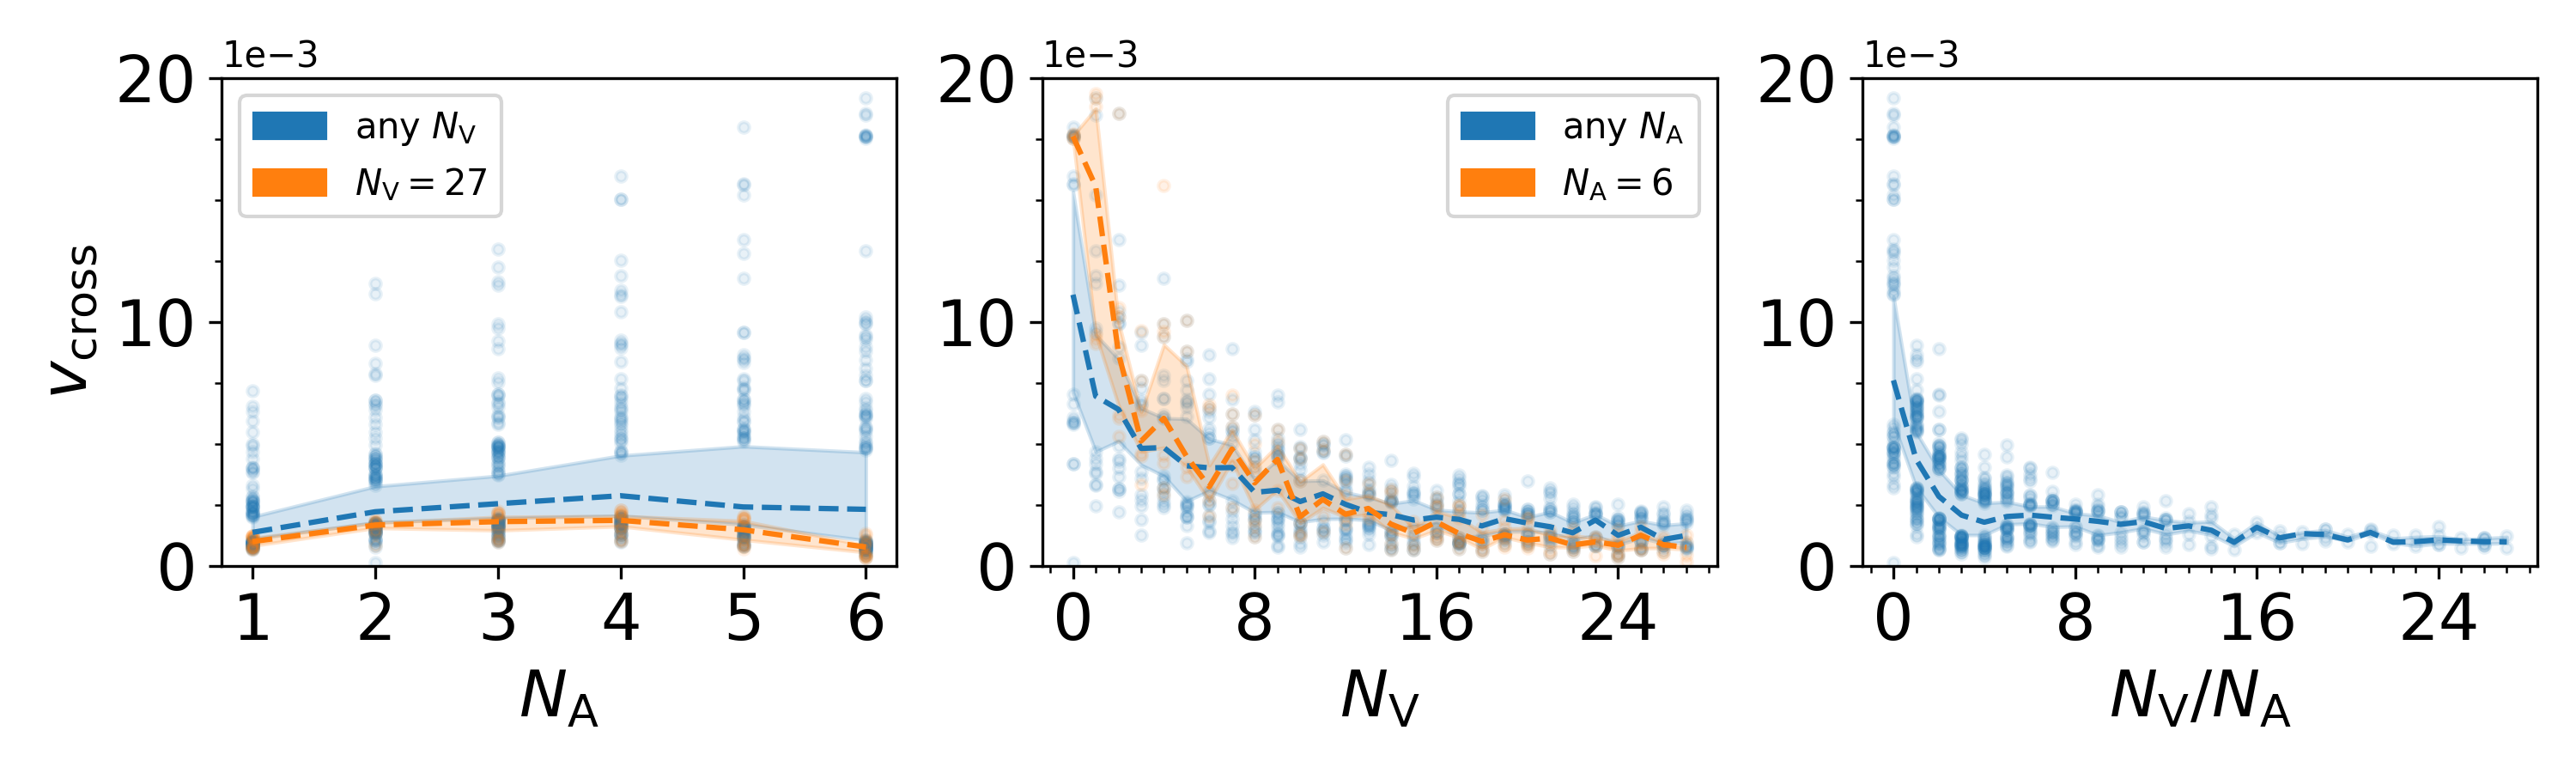
\includegraphics[width=\textwidth]{diagrams/results-variations/mega4_no-arteries_no-veins_veins-to-arteries.png}
                \caption{Graphs that show how $v_\text{cross}$ varies with changes in the number of arteries and veins. The first column plots these measures for varying the number of arteries from $1$ to $6$, the second column plots these measures for varying the number of veins from $0$ to $27$, and the third column plots these measures for the ratio between the number of veins and the number of arteries. In each panel, the dotted lines correspond to the median, and the surrounding shaded regions correspond to the area between the $25$th and $75$th percentile of the data, with individual outlier points plotted outside these regions. Blue data points correspond to all $N_\text{sim}$ simulations, whereas orange data points are some subset of this data.}
                \label{fig:mega-vessels4}
            \end{figure}
            
            Increasing $N_\text{A}$ has an interesting influence on $v_\text{cross}$ in that the median plotted in blue is non-monotonic, with the maximum median value attained at roughly $N_\text{A} = 4$. The orange curve for $N_\text{V} = 27$ makes this even clearer, with almost no cross-flow flux at all when $N_\text{V} = 27$ and $N_\text{A} = 6$; this suggests that high $v_\text{cross}$ benefits from more arteries (giving overall more flow) and strongly asymmetric artery placement (roughly speaking, when $N_\text{A} \neq 6$). That said, both the number of outlier points and the shaded blue area drastically increase in size for higher $N_\text{A}$, showing that the variability is also increasing here; this is due to variations in $N_\text{V}$ dominating the value of $v_\text{cross}$.
            
            Turning our attention to the second and third columns we learn that, like the effects on venous drainage, $N_\text{V}$ has by far the most influence on cross-placentone flux here. When $N_\text{V}$ is small, there is a high amount of variability in where those veins are positioned, which in extreme cases could be placed far from arteries. In these cases, assuming a negligible amount of drainage through the marginal sinus veins, blood would be drawn over several septal walls to exit through those veins. In contrast, when $N_\text{V}$ is high, there is a high likelihood that veins are close to arteries, allowing blood to easily exit through nearby veins. This further reinforces the idea of short-circuiting being commonly available when $N_\text{V}$ is high.

        \subsection{Effects on kinetic energy flux}
            We finally discuss the effects of vessel variations on $E_\text{kinetic}$ in Figure \ref{fig:mega-vessels5}. We will specifically study the energy flux loss ratio (EFLR), which is calculated by
            \begin{equation*}
                \frac{E_\text{kinetic}(\Gamma_\text{in}) - E_\text{kinetic}(\Gamma_\text{out})}{E_\text{kinetic}(\Gamma_\text{in})}.
            \end{equation*}
            This gives a measure of how kinetic energy is lost as the blood passes through the villous tree.

            \begin{figure}
                \centering
                % Date generated: 2024-09-25 21:00:03
                % Commit: 6f2093f52291a15fff9408dbc5b0eff090c5f72f
                % File run: ./drivers/variations_2024-03-21/vary_mega-vessels.py
                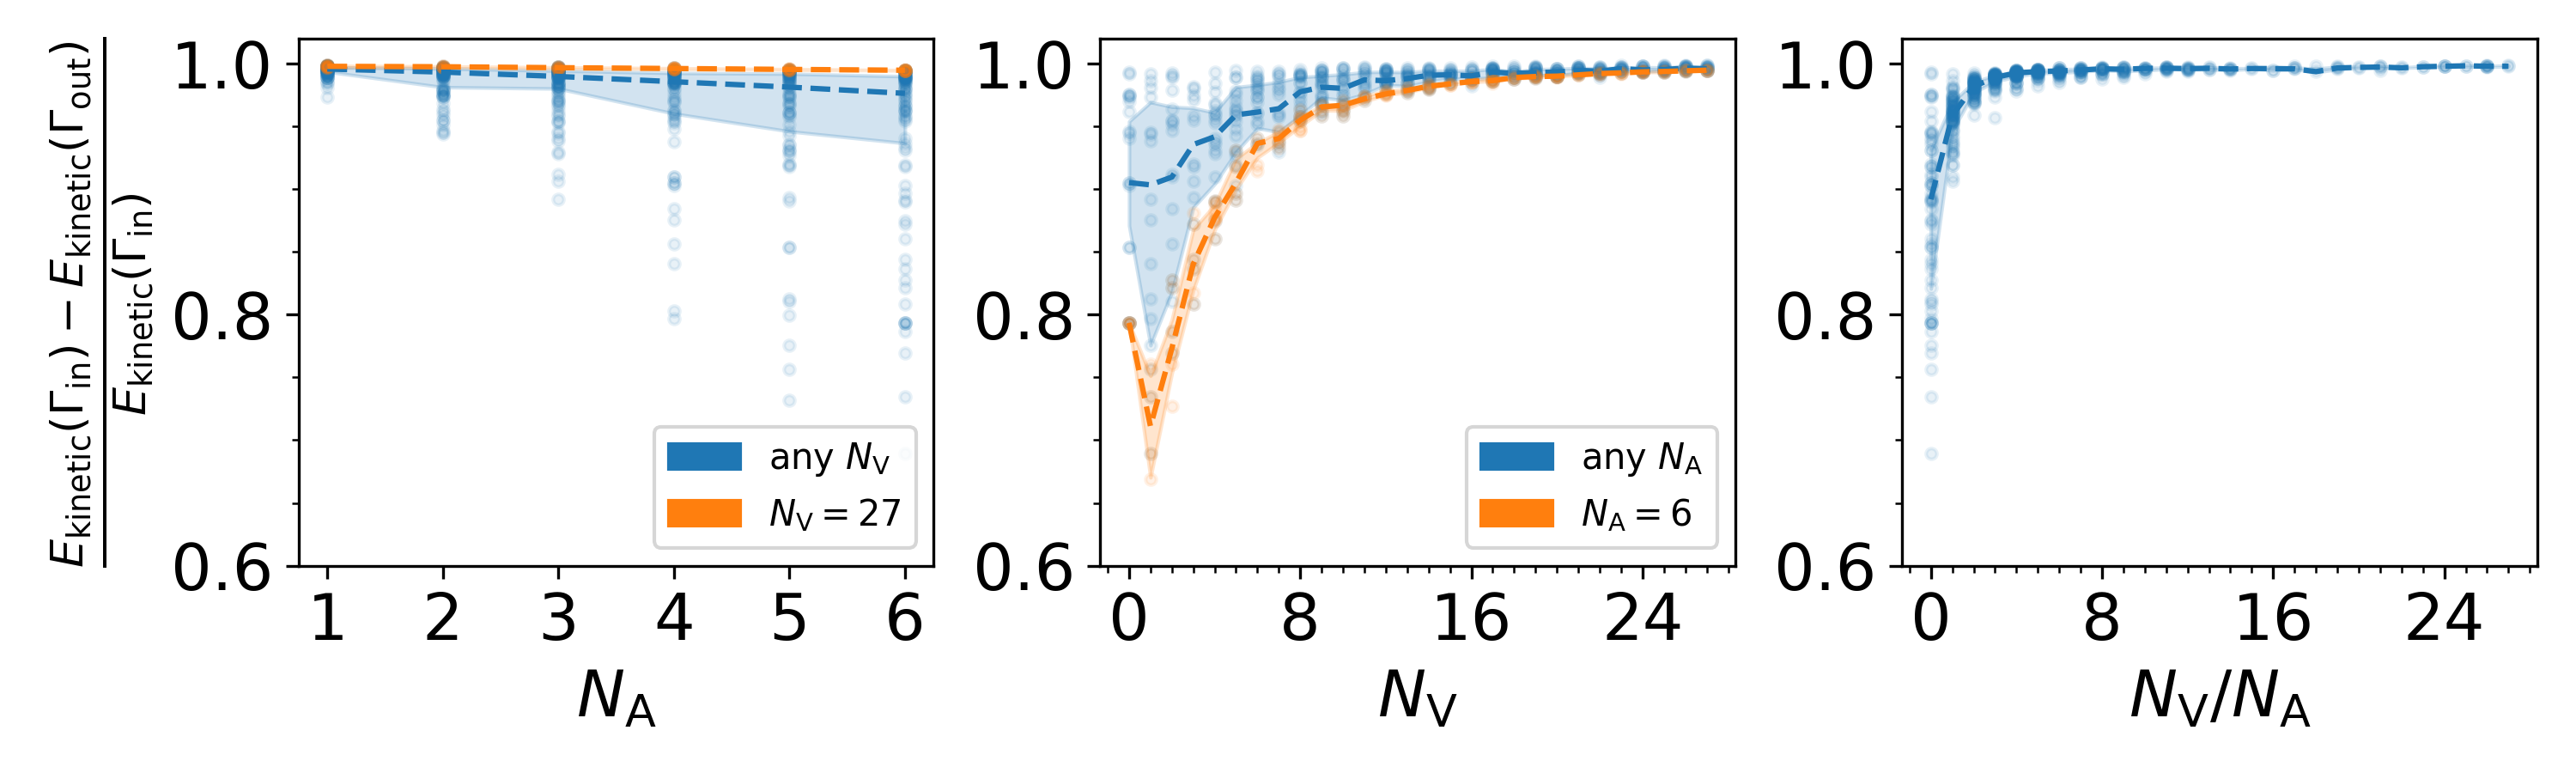
\includegraphics[width=\textwidth]{diagrams/results-variations/mega5_no-arteries_no-veins_veins-to-arteries.png}
                \caption{Graph that shows how $E_\text{kinetic}$ varies with changes in the number of arteries and veins. The first column plots these measures for varying the number of arteries from $1$ to $6$, the second column plots these measures for varying the number of veins from $0$ to $27$, and the third column plots these measures for the ratio between the number of veins and the number of arteries. In each panel, the dotted lines correspond to the median, and the surrounding shaded regions correspond to the area between the $25$th and $75$th percentile of the data, with individual outlier points plotted outside these regions. Blue data points correspond to all $N_\text{sim}$ simulations, whereas orange data points are some subset of this data.}
                \label{fig:mega-vessels5}
            \end{figure}
            
            % The main motivation for studying the kinetic energy flux $E_\text{kinetic}$ is because we can derive an analytical expression for how this ought to behave for difference numbers of arteries and veins. We will study the energy flux loss ratios (EFLRs), which for the kinetic and total energy are respectively calculated by
            % \begin{equation*}
            %     \frac{E_\text{kinetic}(\Gamma_\text{in}) - E_\text{kinetic}(\Gamma_\text{out})}{E_\text{kinetic}(\Gamma_\text{in})},
            % \end{equation*}
            % \begin{equation*}
            %     \frac{E_\text{total}(\Gamma_\text{in}) - E_\text{total}(\Gamma_\text{out})}{E_\text{total}(\Gamma_\text{in})}.
            % \end{equation*}

            % Before we interpret the results of our simulations, we will briefly introduce the main ideas behind deriving an analytical expression $\Phi$ for describing the relationship between the kinetic EFLR and the number of vessels in the placenta. To be clear,
            % \begin{equation*}
            %     \Phi(N_\text{A}, N_\text{V}) \approx \frac{E_\text{kinetic}(\Gamma_\text{in}) - E_\text{kinetic}(\Gamma_\text{out})}{E_\text{kinetic}(\Gamma_\text{in})},
            % \end{equation*}
            % and is defined as
            % \begin{equation}
            %     \Phi(N_\text{A}, N_\text{V}) = \frac{N_\text{A} - 3N_\text{V}K-1^2 - 12k_2^2}{N_\text{A}},
            %     \label{eq:kinetic-energy-relationship}
            % \end{equation}
            % where
            % \begin{align*}
            %     k_1 & = \frac{N_a}{3(2+N_v)}, \\
            %     k_2 & = \frac{k_1}{4}.
            % \end{align*}
            % The derivation of $\Phi$ is outlined in \S\ref{??}.

            The most straightforward relationship is the one for varying $N_\text{A}$ in the first column; we see that for increasing $N_\text{A}$, there is a relatively small decrease in the energy measure shown in blue, with an even smaller decrease visible when fixing $N_\text{V} = 27$ in orange. For the data points for any choice of $N_\text{V}$ in blue, there is a higher variability as $N_\text{A}$ increases, which is due to simulations with small $N_\text{V}$ having a large effect there; this is especially evident through the fact that there is not a high variability for $N_\text{V} = 27$ and there is a much larger change in behaviour for lower numbers of veins, as previously discussed.

            Focussing now on the second column for varying $N_\text{V}$, we see that there is non-monotonic behaviour for increasing $N_\text{V}$: the energy briefly decreases from $N_\text{V} = 0$ to low $N_\text{V}$, but then increases up to a plateau for a larger number of veins. The visualisation for $N_\text{A} = 6$ in orange exaggerates this behaviour, which has an even sharper decrease in value for smaller numbers of veins. This is interesting behaviour, as it suggests that there is a unique situation present in the flow when $N_\text{V}$ is small that overall expels more kinetic energy between entering and exiting the placenta.
            
            % Physically, this can be explained by referring back to the purple-boxed simulation in Figure \ref{fig:mega-vessels1:simulations}, where there is only one septal wall vein present; clearly, the majority of the fast (and high kinetic energy) flow is concentrated near this septal wall vein in this particular simulation, with much lower overall kinetic energy present elsewhere in the domain. For $N_\text{V} = 0$, flow would instead be faster over more of the domain as it would be drawn towards the two marginal sinus veins, and for higher numbers of veins, there would be more opportunity for flow to remain locally fast and short-circuit. Therefore, in the case where $N_\text{V}$ is small, we have a unique situation where there is a balance between highly kinetic flow exiting through nearby veins, and a smaller amount of highly kinetic flow no longer reaching marginal sinus veins.
            
            %Interestingly, this behaviour is captured by $\Phi$, which also predicts a sharp decrease before smoothly increasing up to the plateau.

            % The behaviour of these EFLRs in our study of the placenta is quite different from the previous studies on the heart \cite{rijnbergEnergeticsBloodFlow2018,whiteheadNonlinearPowerLoss2007}; high values of EFLRs are associated with efficient cardiac output, whereas low values of EFLRs suggest energy has been unnecessarily wasted through, for example, turbulent flow, which results in reduced cardiac output. The behaviour of these EFLRs in our results show that the placenta expels almost all of the incoming energy for almost all choices of $N_\text{A}$ and $N_\text{V}$, due to 

            We will now assume that the number and position of all vessels are fixed, and instead consider variations in seven different parameters.

    \section{Variation of seven other parameters} \label{sec:nutrient-uptake:variation-of-other-parameters}        
        Similar to \S\ref{sec:nutrient-uptake:variation-of-vessels}, we will vary structural parameters to investigate their effects on the seven chosen measures of efficiency. Specifically, we will separately investigate the effects due to variations in artery mouth widths ($r_a$), vein widths ($r_v$), septal wall heights ($h$), oxygen diffusivity ($D$), oxygen uptake rate ($R$), maximum permeability of the IVS ($k$), and inlet blood flow speed ($U$). Note that the number and position of the vessels remain fixed in this study and are positioned in the same way as the simulations presented in \S\ref{sec:numerical-methods:blood-flow-experiments:comparison} (i.e., 1 artery and 2 basal plate veins per placentone). This is a constraint that may affect our results, but was chosen because of its similarity to the position and number of vessels that have previously been used in the mathematical modelling literature \cite{lecarpentierComputationalFluidDynamic2016,chernyavskyMathematicalModelIntervillous2010}.
        
        We vary the artery mouth widths from $2r_a = \qty{0.5}{\milli\metre}$ (no widening of artery) to $2r_a = \qty{3}{\milli\metre}$ \cite{burtonRheologicalPhysiologicalConsequences2009}; we recall from Table \ref{tab:structural-parameters} that the nominal value for the artery width used elsewhere in this thesis is $2r_a = \qty{2.4}{\milli\metre}$. Similarly, we vary the vein widths from $2r_v = \qty{1}{\milli\metre}$ and $2r_v = \qty{3}{\milli\metre}$, where we recall that the nominal width is $2r_v = \qty{1.5}{\milli\metre}$. We take the septal wall heights to vary at fractions of $h/h_0 = 1/3$ and $h/h_0 = 2$ times their original heights from Table \ref{tab:structural-parameters}\footnote{This involves the small and tall walls respectively varying \qtyrange{2.30}{13.80}{\milli\metre} and \qtyrange{4.69}{28.14}{\milli\metre}.}. For the oxygen diffusivity and oxygen uptake rate, we vary these from $0.1$ and $5$ times their nominal values; this involves varying between $D = \qty{1.667e-10}{\milli\metre^2\per\second}$ and $D = \qty{8.335e-9}{\milli\metre^2\per\second}$, and $R = \qty{1.667e-3}{\per\second}$ and $R = \qty{8.335e-2}{\per\second}$. We follow work by \citeauthor{lecarpentierComputationalFluidDynamic2016} \cite{lecarpentierComputationalFluidDynamic2016} and choose to vary the maximum permeability between $k = \qty{1e-10}{\metre^2}$ and $k = \qty{1e-6}{\metre^2}$. Finally, we follow the work of references \cite{burtonRheologicalPhysiologicalConsequences2009,saghianAssociationPlacentalJets2017,chernyavskyMathematicalModelIntervillous2010} and choose to vary the inlet blood speed between $U = \qty{0.1}{\metre\per\second}$ and $U = \qty{1}{\metre\per\second}$, where we recall that the nominal speed is $U = \qty{0.35}{\metre\per\second}$.
        
        The algorithm for generating these simulations is much more straightforward than in \S\ref{sec:nutrient-uptake:variation-of-vessels}, as we choose to keep the numbers and positions of vessels as they are presented in \S\ref{sec:modelling:geometries:2d-placenta}. Specifically, the variations in each of these parameters are chosen uniformly on the ranges described above and simulations run with these chosen parameters\footnote{Due to the behaviour of the permeability, we select the permeabilities logarithmically uniformly, i.e., $k \sim 10^{X}, X \sim \mathcal{U}(-10, -6)$.}. We run $N_\text{sim} = 1000$ simulations for \textit{each} of these seven parameter variations ($7000$ total simulations). Figures \ref{fig:mega-other1} and \ref{fig:mega-other2} present the main results of \S\ref{sec:nutrient-uptake:variation-of-other-parameters} for all seven efficiency measures, which we will discuss throughout the remainder of \S\ref{sec:nutrient-uptake:variation-of-other-parameters}; we highlight that the simulations presented in each of the seven columns are a \textit{different} ensemble of simulations, in contrast to the results presented in \S\ref{sec:nutrient-uptake:variation-of-vessels}. We make clear that the choice of seven \textit{parameters} and seven \textit{efficiency measures} is a coincidence.

        The most striking feature of Figures \ref{fig:mega-other1} and \ref{fig:mega-other2} is that almost all the efficiency measures change very little due to variations in each of the seven parameters compared to the vessel variations. We split the discussion into two parts: \S\ref{sec:nutrient-uptake:variation-of-other-parameters:1} will discuss the results of Figure \ref{fig:mega-other1}, and \S\ref{sec:nutrient-uptake:variation-of-other-parameters:2} will discuss the results of Figure \ref{fig:mega-other2}.

        \subsection{Effects due to geometrical variations} \label{sec:nutrient-uptake:variation-of-other-parameters:1}
            Here, we focus on the results of Figures \ref{fig:mega-other1:1} and \ref{fig:mega-other1:2}, which in each column separately considers variations in artery width, vein width, and septal wall height for all seven efficiency measures.

            \begin{figure}
                \vspace{-1.5cm}
                % Date generated: 2024-09-25 21:00:03
                % Commit: 6f2093f52291a15fff9408dbc5b0eff090c5f72f
                % File run: ./drivers/variations_2024-03-21/vary_mega-others.py
                \centering
                \begin{subfigure}{\textwidth}
                    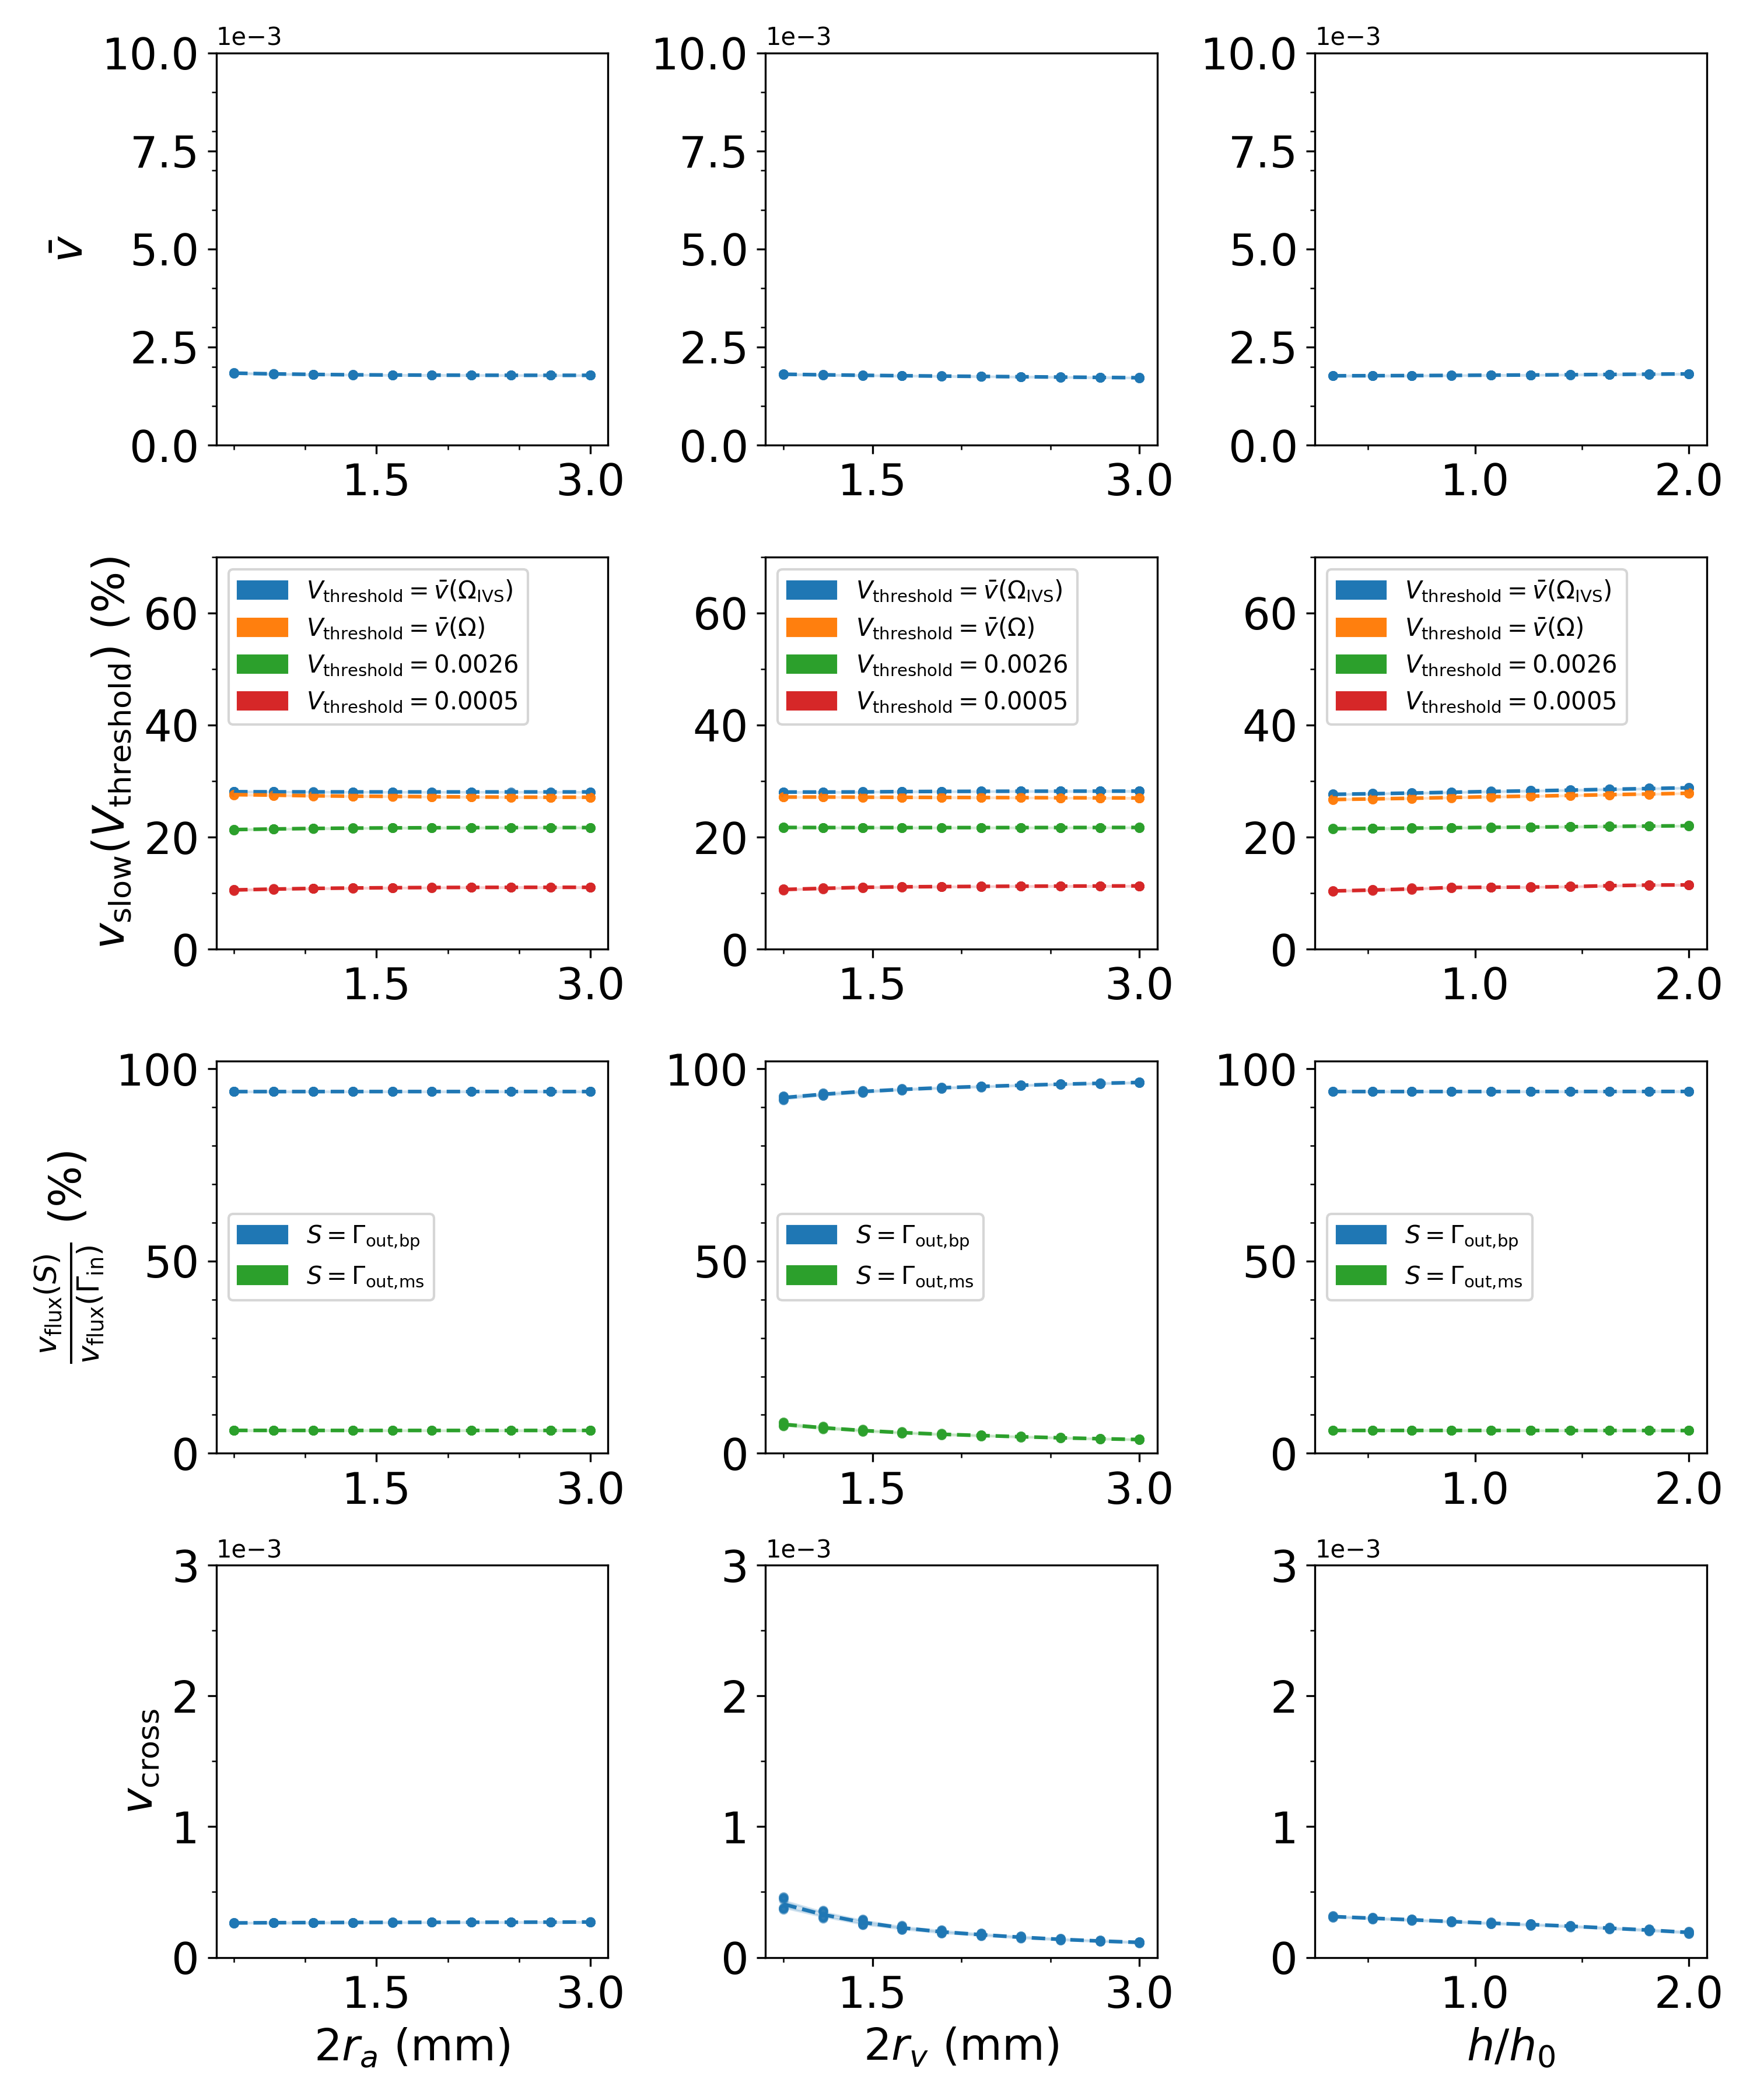
\includegraphics[width=\textwidth]{diagrams/results-variations/mega1_artery_width_vein_width_wall_height_ratio.png}
                    \caption{}
                    \label{fig:mega-other1:1}
                \end{subfigure}
                \caption{Graphs that show how each of the seven measures of placental efficiency from \S\ref{sec:nutrient-uptake:measures-of-efficiency} vary with changes in three different structural parameters. The seven rows are labelled the $y$-axis, utilising each of the efficiency measures once. In each panel, the dotted lines correspond to the median, and the surrounding shaded regions correspond to the area between the $25$th and $75$th percentile of the data, with individual outlier points plotted outside these regions. In panels that contain a legend, each colour indicates a different quantity computed on the vertical axis. The first column plots these measures for varying spiral artery mouth width, the second column plots these measures for varying vein width, and the third column plots these measures for different proportions of original wall height. (a) Presents the results including the first four efficiency measures: $\bar{v}$, $v_\text{slow}$, $v_\text{flux}$, and $v_\text{cross}$. (continued on next page)}
            \end{figure}
            \begin{figure}\ContinuedFloat
                \centering
                \begin{subfigure}{\textwidth}
                    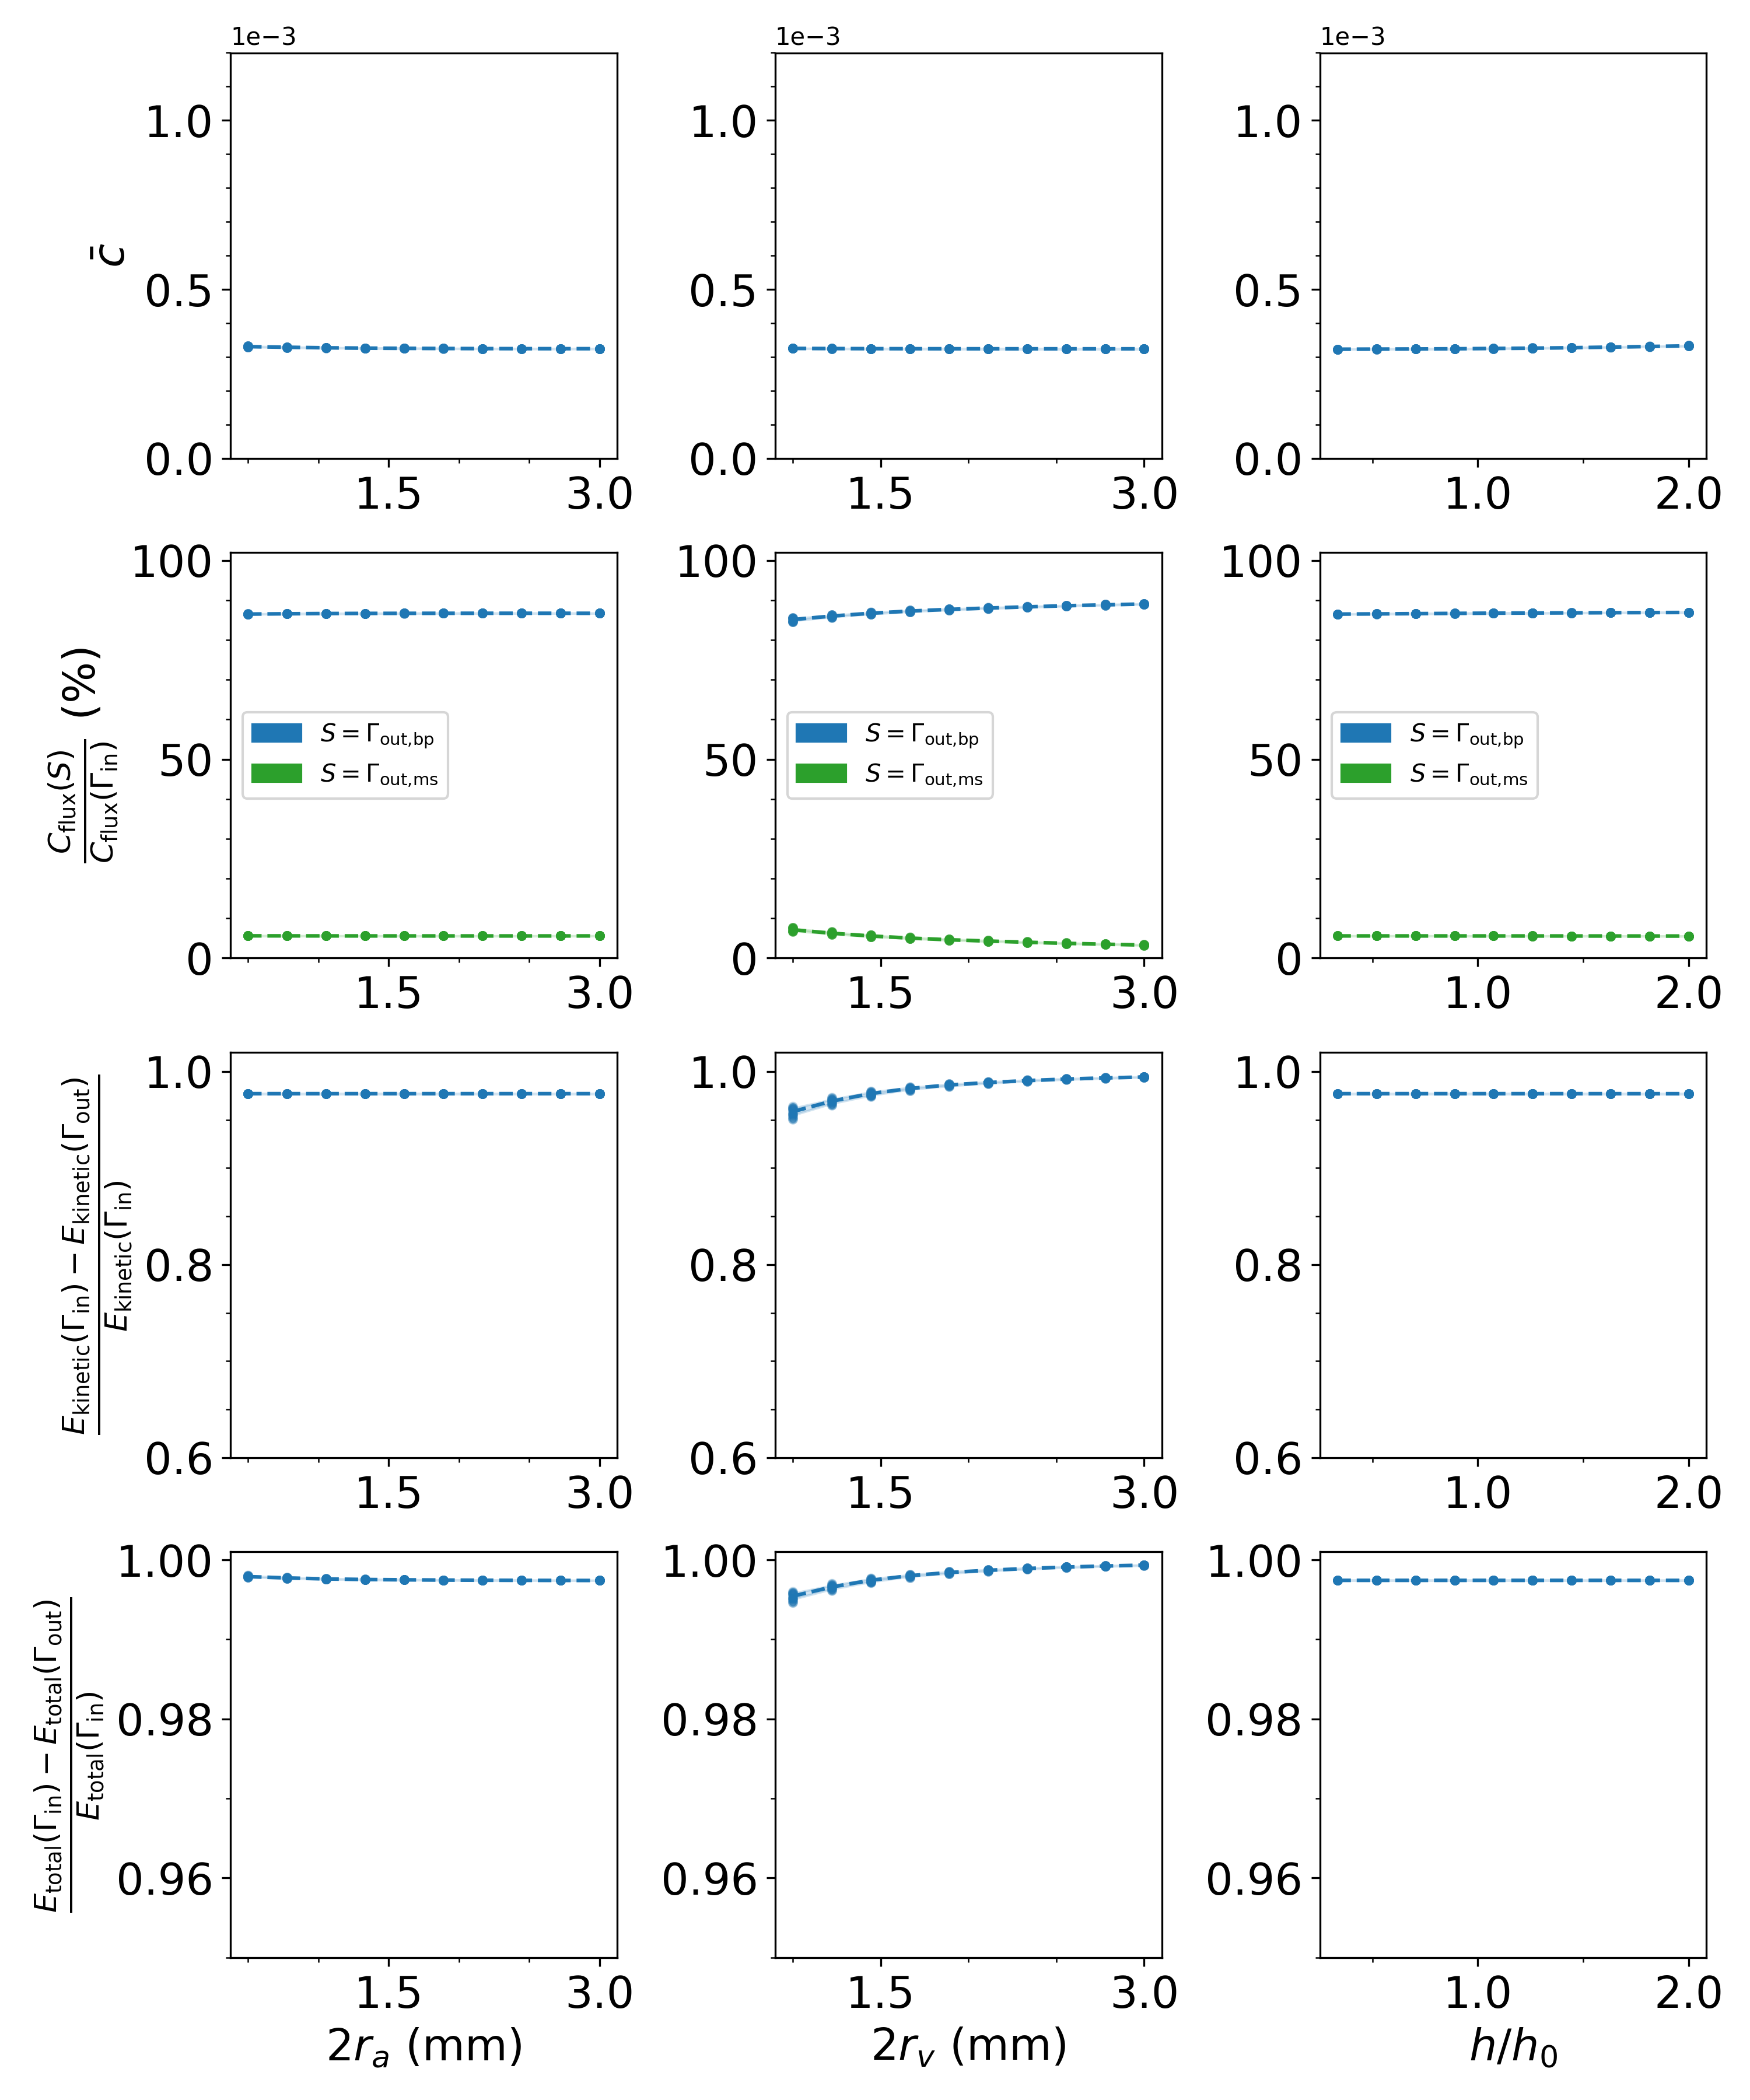
\includegraphics[width=1\textwidth]{diagrams/results-variations/mega2_artery_width_vein_width_wall_height_ratio.png}
                    \caption{}
                    \label{fig:mega-other1:2}
                \end{subfigure}
                \caption{(continued) (b) Presents the results including the next three efficiency measures: $\bar{c}$, $c_\text{flux}$, and $E_\text{kinetic}$.}
                \label{fig:mega-other1}
            \end{figure}

            % Artery widths.
            In the first column, artery width variations have by far the least impact on the efficiency measures out of these three parameters. We note that the variations we have performed here vary all six artery widths simultaneously, and change only the artery mouth width, not the artery width at the base on $\Gamma_\text{in}$; we are therefore not affecting the flux of blood entering through the arteries, instead affecting only the speed at which it exits into the central cavity. However, this is still unexpected, as other studies have suggested that small artery mouth widths would substantially increase flow rates and decrease overall oxygen uptake \cite{burtonRheologicalPhysiologicalConsequences2009}.

            % Vein widths.
            In the second column, we vary the vein widths. We remind the reader that in this particular setup, there are no septal wall veins, and we specifically perform variations in the basal plate vein widths along their entire lengths, which therefore affects the size of both the mouth and base of these veins. The third row of Figure \ref{fig:mega-other1:1} and the second row of Figure \ref{fig:mega-other1:2} show in the second column that smaller vein widths lead to more flow to exit out of the marginal sinus, with correspondingly higher concentrations of oxygen. This behaviour is due to a slight preference for the flow to exit through the much wider (\qty{3}{\milli\metre}) marginal sinus veins when the basal plate veins are small. It therefore makes sense that for small vein widths that $v_\text{cross}$ is also elevated, as flow will be drawn across the domain in this case. A final related feature is present in the kinetic EFLR (energy flux loss ratio), which is lowered for smaller vein widths. This is again due to the preference for the marginal sinus veins, and mirrors the results discussed in \S\ref{sec:nutrient-uptake:variation-of-vessels} when the marginal sinus vein drainage was preferred.

            % Septal wall height.
            We recall that the variations to septal wall heights are ratios ($h/h_0$) between $1/3$ and $2$ times their nominal heights ($h_0$), which are chosen at one of two sizes: one taller height to represent wall heights between lobes, and another smaller height to represent wall heights between lobules (see Figure \ref{fig:inverted-circle-slice-6-flat:dimensions} and accompanying discussion in \S\ref{sec:modelling:geometries:2d-placenta}). Like artery width, septal wall heights have very little impact on the seven measures of placental efficiency, with the only notable effect that $v_\text{cross}$ decreases for increasing septal wall height. This makes physical sense, as for taller wall heights, there will be a smaller gap between the walls and the chorionic plate for flow to pass through, which could therefore decrease the overall flux of blood crossing between placentones. However, it is not obvious that this would have such a small influence on the other efficiency measures. The small influence is due to the relatively low-speed flow passing over the walls, which have previously been visualised with logarithmically-scaled colours.

            % Summary.
            Overall, these parameter variations had a much smaller effect on the efficiency measures compared to the vessel variations presented in \S\ref{sec:nutrient-uptake:variation-of-vessels}. Surprisingly, the only parameter variation that had a discernable effect was the vein widths, which is due to the larger marginal sinus veins being preferred. It was unexpected that artery widths influenced the measures very little, given that studies have previously suggested that non-widening arteries are likely to have a significant effect on placental function \cite{burtonRheologicalPhysiologicalConsequences2009}. We will give a discussion on this feature in \S\ref{sec:nutrient-uptake:summary}. We also found that variations in the wall height had little effect on the measures; although $v_\text{cross}$ decreased slightly for increasing wall height, there was no other obvious disruption to the flow and oxygen concentration fields, due to the relatively low-speed flow.

            Next, we will consider the results of Figure \ref{fig:mega-other2}.

        \subsection{Effects due to changes to the villous tree, oxygen diffusivity, and inlet blood speed} \label{sec:nutrient-uptake:variation-of-other-parameters:2}
            Here, we focus on the results of Figures \ref{fig:mega-other2:1} and \ref{fig:mega-other2:2}, which in each column separately considers variations in oxygen diffusivity, oxygen uptake rate, maximum permeability of the villous tree, and the inlet blood flow speed for all seven efficiency measures. We remark that panels containing flow markers for variations in the oxygen concentration field are hidden, as they are not affected by the variations; this is because changes in $D$ and $R$ only affect $c$, not $\vec{u}$.

            \begin{figure}
                % Date generated: 2024-09-25 21:00:03
                % Commit: 6f2093f52291a15fff9408dbc5b0eff090c5f72f
                % File run: ./drivers/variations_2024-03-21/vary_mega-others.py
                \hspace{-0.8cm}
                \centering
                \begin{subfigure}{\textwidth}
                    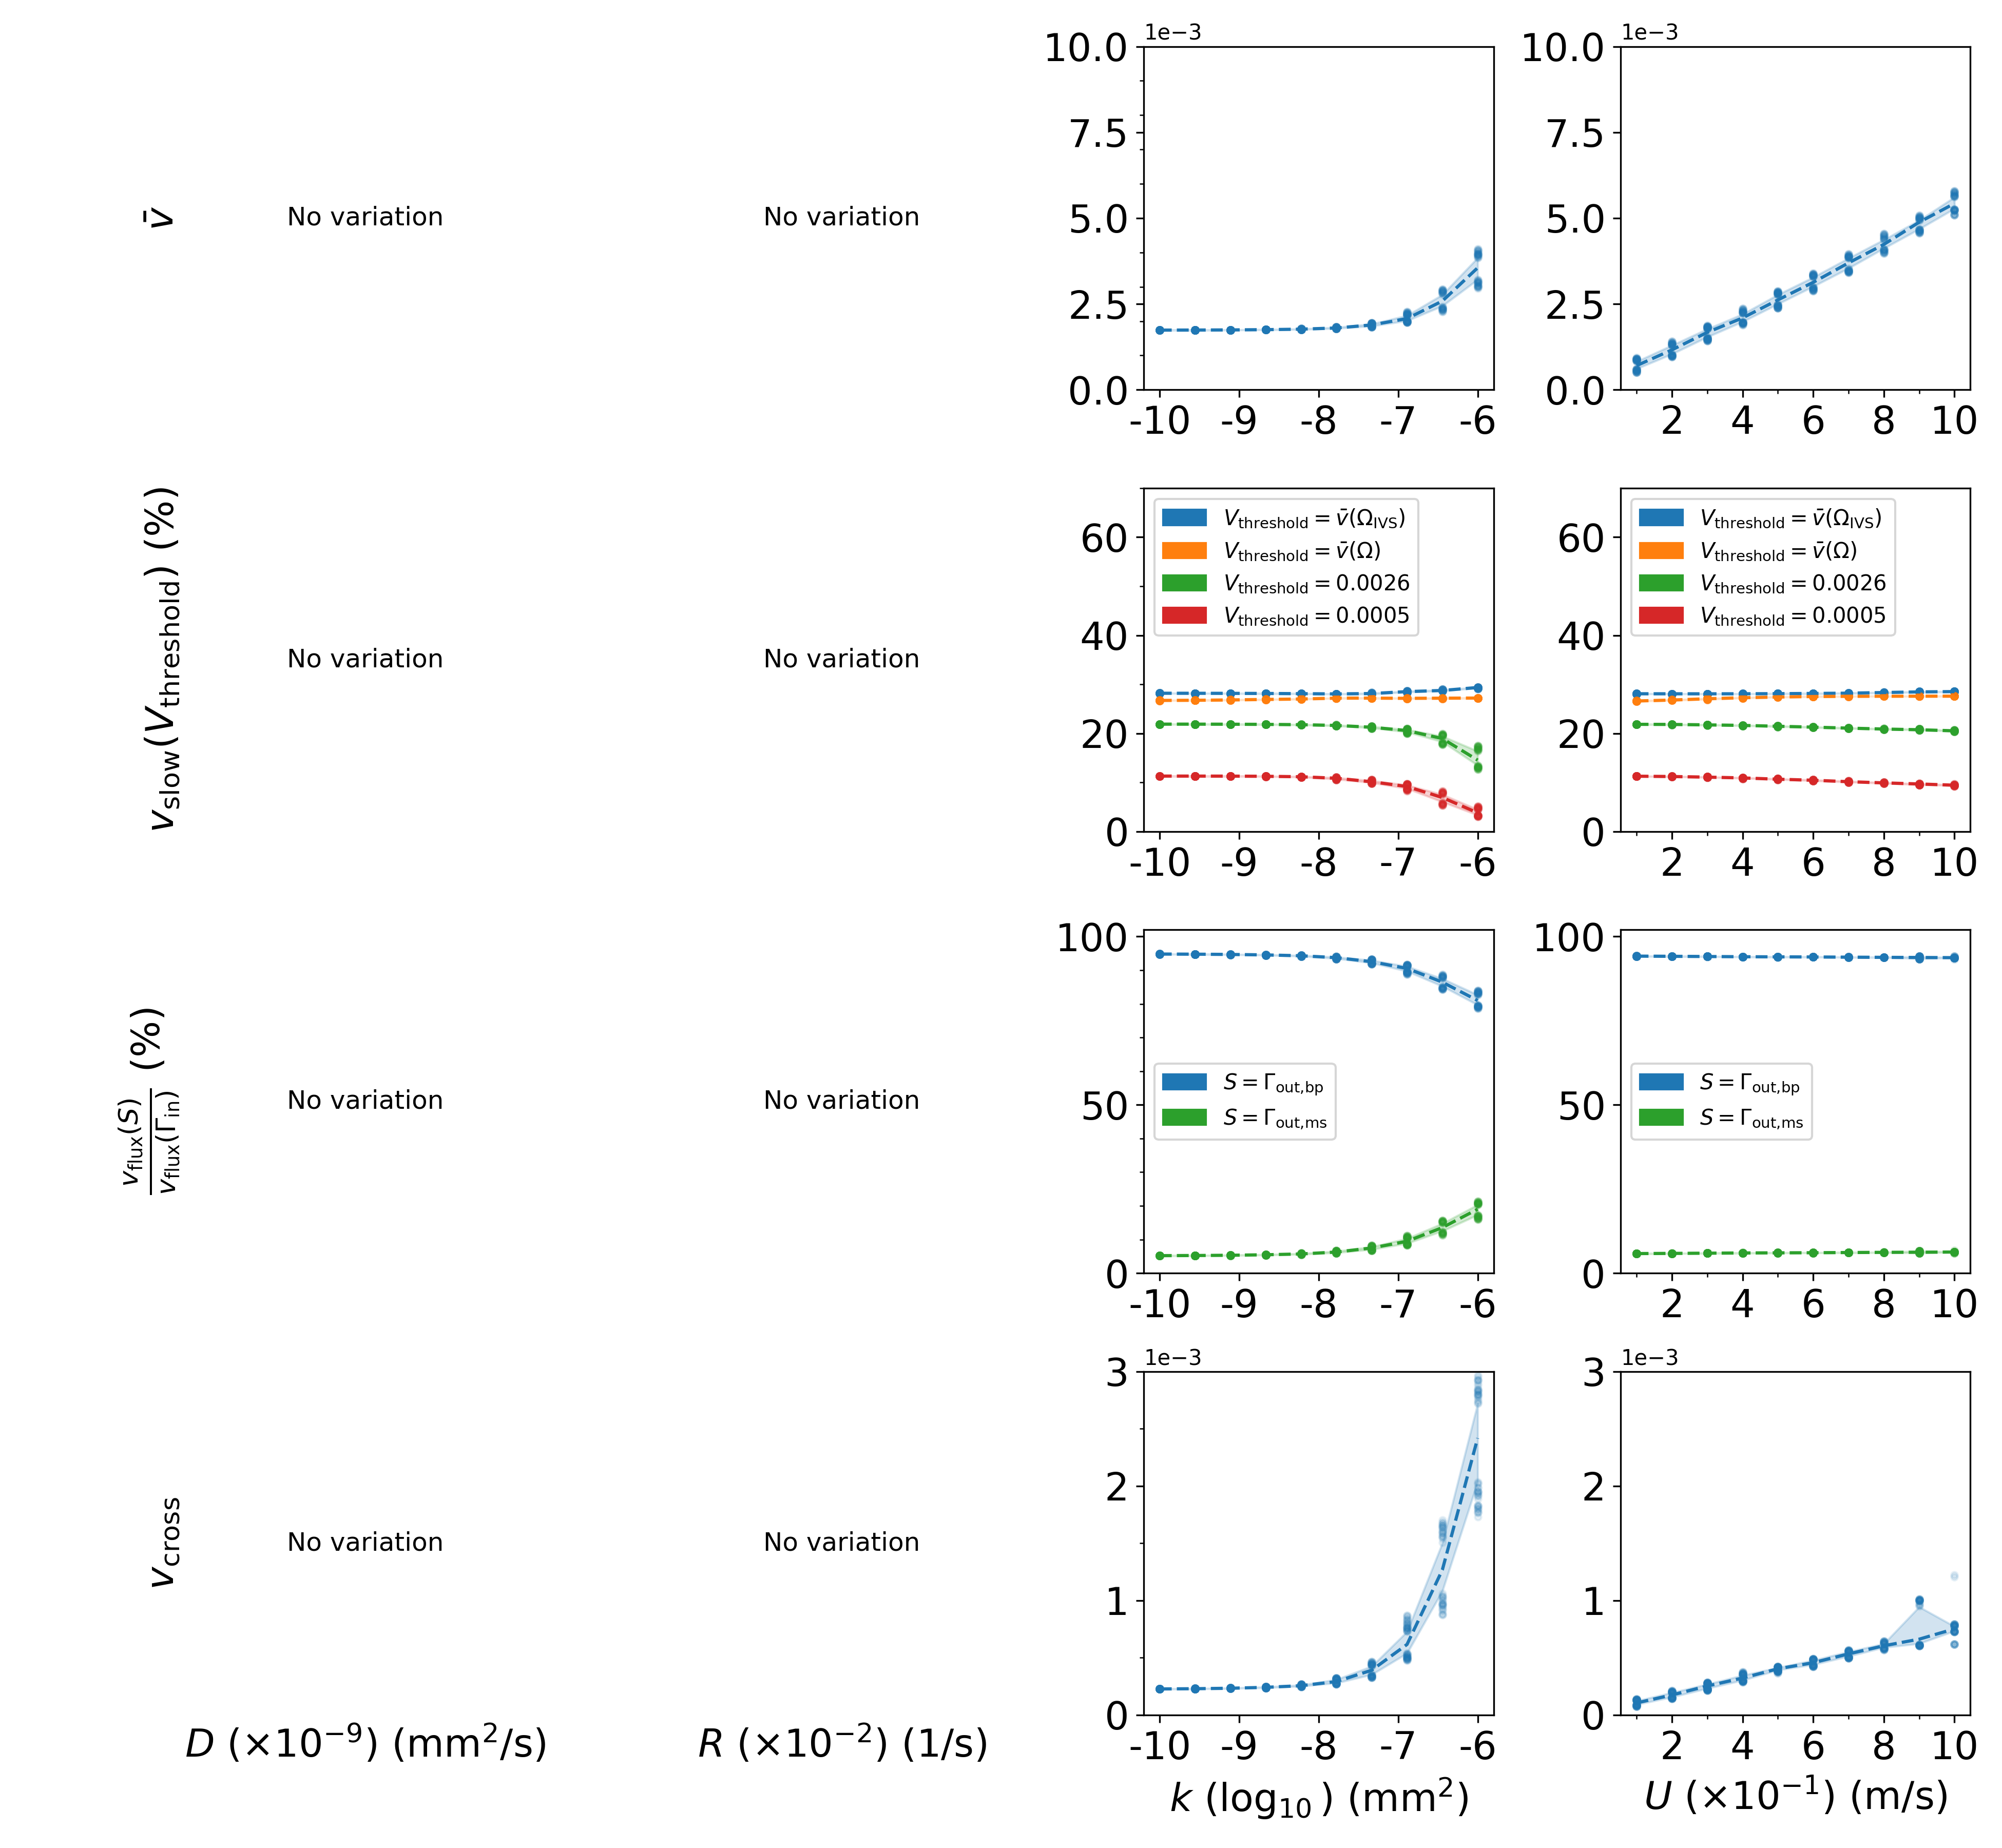
\includegraphics[width=1.0\textwidth]{diagrams/results-variations/mega1_oxygen_diffusivity_oxygen_uptake_permeability_inlet_velocity.png}
                    \caption{}
                    \label{fig:mega-other2:1}
                \end{subfigure}
                \caption{Graphs that show how each of the seven measures of placental efficiency from \S\ref{sec:nutrient-uptake:measures-of-efficiency} vary with changes in four different flow and structural parameters. The seven rows are labelled the $y$-axis, utilising each of the efficiency measures once. In each panel, the dotted lines correspond to the median, and the surrounding shaded regions correspond to the area between the $25$th and $75$th percentile of the data, with individual outlier points plotted outside these regions. In panels that contain a legend, each colour indicates a different quantity computed on the vertical axis. The first column plots these measures for varying oxygen diffusivity, the second column plots these measures for varying oxygen uptake rate, the third column plots these measures for varying permeability of the villous tree, and the fourth column plots these measures for varying inlet blood speed. Note that panels containing flow markers are hidden for variations in the oxygen concentration model. (a) Presents the results including the first four efficiency measures: $\bar{v}$, $v_\text{slow}$, $v_\text{flux}$, and $v_\text{cross}$. (continued on next page)}
            \end{figure}
            \begin{figure}\ContinuedFloat
                \hspace{-1.9cm}
                \centering
                \begin{subfigure}{\textwidth}
                    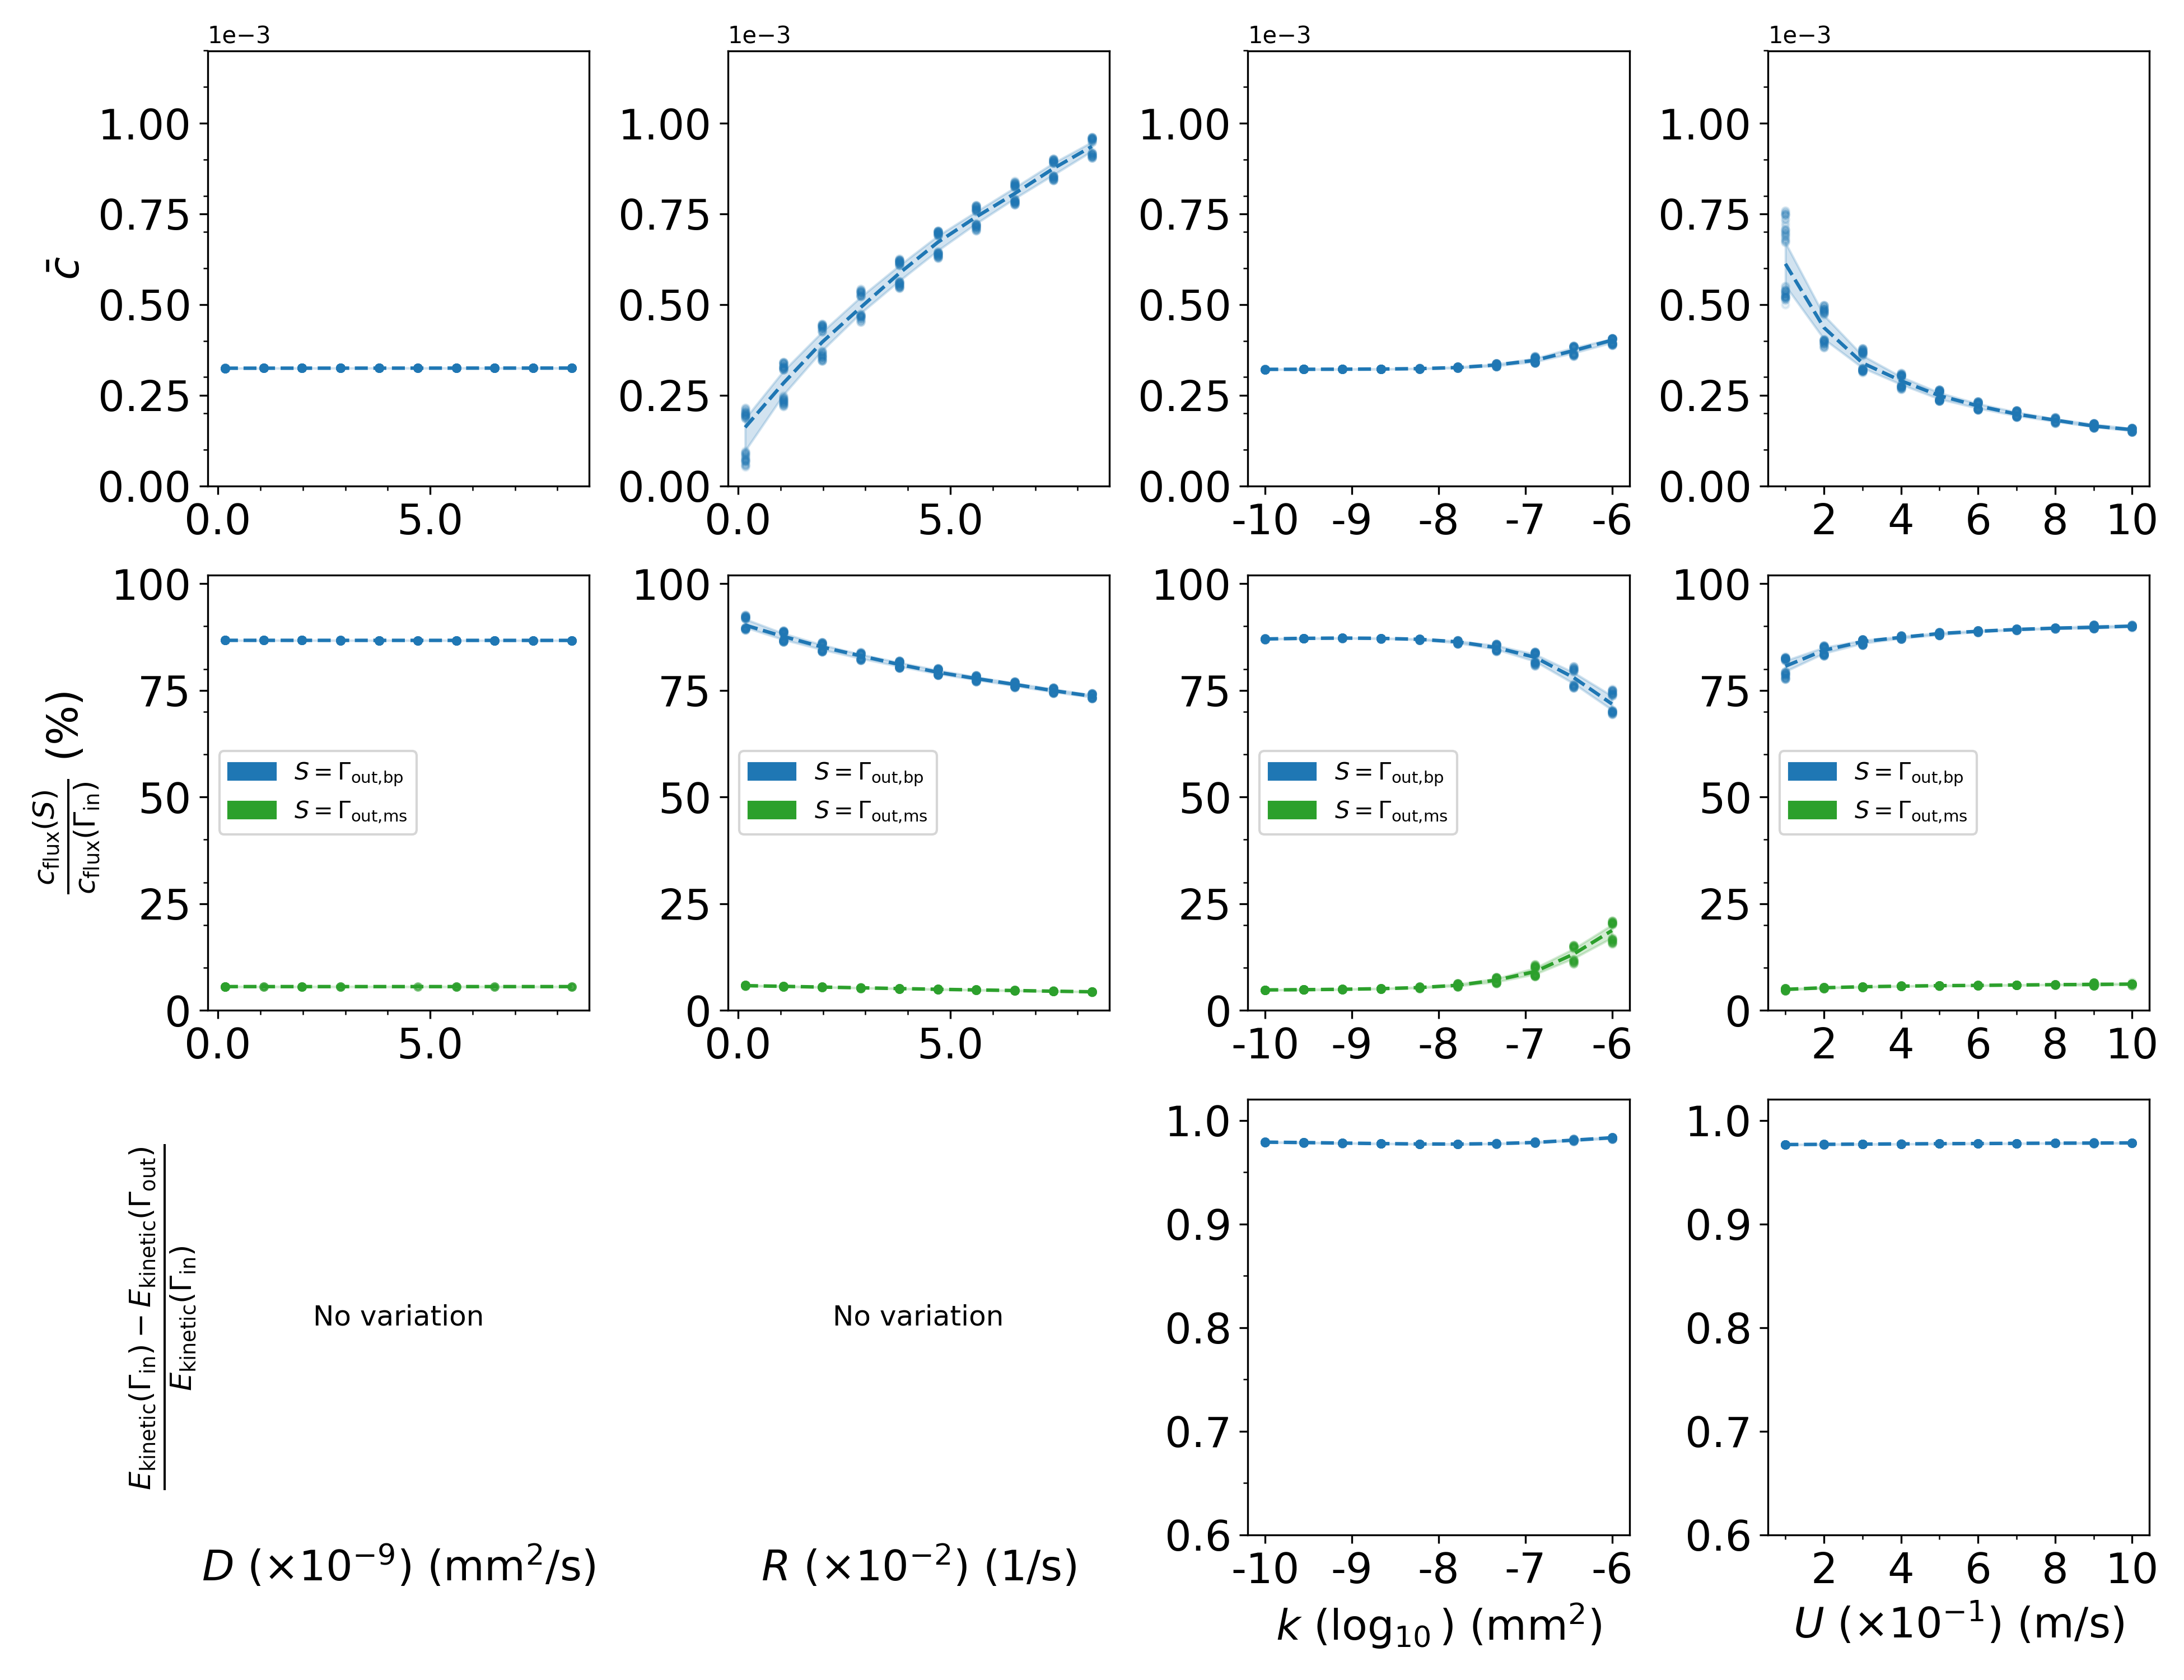
\includegraphics[width=1.1\textwidth]{diagrams/results-variations/mega2_oxygen_diffusivity_oxygen_uptake_permeability_inlet_velocity.png}
                    \caption{}
                    \label{fig:mega-other2:2}
                \end{subfigure}
                \caption{(continued) (b) Presents the results including the next three efficiency measures: $\bar{c}$, $c_\text{flux}$, and $E_\text{kinetic}$.}
                \label{fig:mega-other2}
            \end{figure}

            % Oxygen diffusivity and oxygen uptake rate
            % * Duffisivity has seemingly no impact -> Chernyavsky 2011
            % * Uptake rate has a direct influence on c and c_flux; understandably has no impact on the other six velocity-based measures.
            The first column of Figures \ref{fig:mega-other2:1} and \ref{fig:mega-other2:2} considers variations in the oxygen diffusivity, which has the smallest effect on the efficiency measures. This suggests that the transport of oxygen here is not diffusion-limited and is instead limited by some other factor in this parameter regime.
            
            We now concentrate on the oxygen uptake rate, shown in the second column of Figures \ref{fig:mega-other2:1} and \ref{fig:mega-other2:2}. The first row of Figure \ref{fig:mega-other2:2} measures $\bar{c}$ and shows a direct increase for increasing oxygen uptake rate, which suggests that the oxygen uptake here is limited by the speed at which the villous tree can absorb oxygen; however, this curve starts to flatten for higher uptake rates, suggesting that for higher uptake rates that there is another limiting factor in uptake in play (for example, instead limited by advection). Related to this, increasing oxygen uptake rate also causes a direct reduction in the oxygen concentration exiting the placenta, as shown in the second row of Figure \ref{fig:mega-other2:2}; this is not surprising and is of course advantageous to placental function.

            % Villous tree permeability
            % * Greatest impact.
            % * v and c
            % * V_slow
            % * V_flux and c_flux
            % * V_cross
            % * Energies
            The third column of Figures \ref{fig:mega-other2:1} and \ref{fig:mega-other2:2} considers variations of $k$, which is the maximum permeability of the villous tree; we recall that the effective resistance to flow is controlled by $\Psi \frac{\mu}{k}$ in Equation \eqref{eq:nsb}. When the resistance to flow is lower (i.e., $k \approx 10^{-6}$), $\bar{v}$ increases due to higher-speed flow penetrating deeper into the IVS; $v_\text{cross}$ and $v_\text{flux}(\Gamma_\text{out,ms})/v_\text{flux}(\Gamma_\text{in})$ both also increase here, due to the deeper penetration of blood, which makes it easier for blood to cross septal walls to then exit through the marginal sinus veins rather than through the basal plate veins. It is not surprising that $v_\text{slow}$ decreases in this regime, with an increase in oxygen exiting through the marginal sinus veins that matches the increase in flow. We also see a small increase in oxygen uptake, which is due to oxygen being transported deeper into the IVS, into regions where there typically is very little oxygen for the villous tree to uptake. The kinetic EFLR remains roughly constant, except for a slight increase when resistance to flow is lower (i.e., $k \approx 10^{-6}$); this is because the fluid experiences more kinetic energy loss when resistance to flow is higher.

            % Blood inlet speed
            % * Better-than-linear increase in v
            % * Little impact on V_slow, V_flux, and E_kinetic
            % * VERY interesting behaviour on V_cross; groups (numbers); citations
            % * Reduction in c for faster inlet speed, as expected; corresponding increase in c_flux
            Finally, we consider the blood inlet speed, shown in the fourth column of Figures \ref{fig:mega-other2:1} and \ref{fig:mega-other2:2}. $\bar{v}$ directly increases for higher $U$, whilst $\bar{c}$ decreases; these phenomena have been reported in the literature, with the reduction in oxygen uptake thought to be due to faster circulation times in which the villous tree has a reduced opportunity in which to uptake oxygen \cite{burtonRheologicalPhysiologicalConsequences2009}. Related to this, there is a corresponding increase in $c_\text{flux}(\Gamma_\text{out,bp})$ for faster inflow; it is not immediately obvious that the oxygen flux through $\Gamma_\text{out,ms}$ remains roughly constant for all values of $U$, although it is clear that is it related to the behaviour of $v_\text{flux}(\Gamma_\text{out,ms})$. Changes in $U$ don't have a considerable impact on $v_\text{slow}$, $v_\text{flux}$, and $E_\text{kinetic}$. However, $v_\text{cross}$ displays a very interesting feature: whilst there is a roughly linear relationship for most choices of $U$, the values of $v_\text{cross}$ illustrated at $U = \qty{0.9}{\metre\per\second}$ do not continue this pattern. In fact, the data itself is partitioned into $v_\text{cross} \in [\num{6.0e-4}, \num{7.1e-4}]$ and $v_\text{cross} \in [\num{9.2e-4}, \num{10.1e-4}]$.

            % Bifurcations.
            To further investigate the behaviour of $v_\text{cross}$ for varying $U$, we visualise the velocity field for one simulation in each of the two groups. Figure \ref{fig:bifurcations:452} shows a simulation with $U = \qty{0.8866}{\metre\per\second}$ and has $v_\text{cross} = \num{6.0e-4}$, and \ref{fig:bifurcations:512} shows a simulation with $U = \qty{0.8850}{\metre\per\second}$ and has $v_\text{cross} = \num{10.1e-4}$. We note that these simulations have been selected due to their similar values of $U$ but contrasting values of $v_\text{cross}$. Figures \ref{fig:bifurcations:452-zoom} and \ref{fig:bifurcations:512-zoom} respectively show a zoomed view of the right-most placentone for these two simulations, where we can see the jets of blood have a preference for either the left or right side of the central cavity, likely due to a bifurcation in the underlying PDE; related to this, we also see fewer streamlines cross the right-most wall in Figure \ref{fig:bifurcations:452} than in Figure \ref{fig:bifurcations:512}, which is why $v_\text{cross}$ is elevated in the latter simulation. This feature will be summarised and discussed further in \S\ref{sec:nutrient-uptake:summary}.

            \begin{figure}
                \centering
                \begin{subfigure}{\textwidth}
                    \centering
                    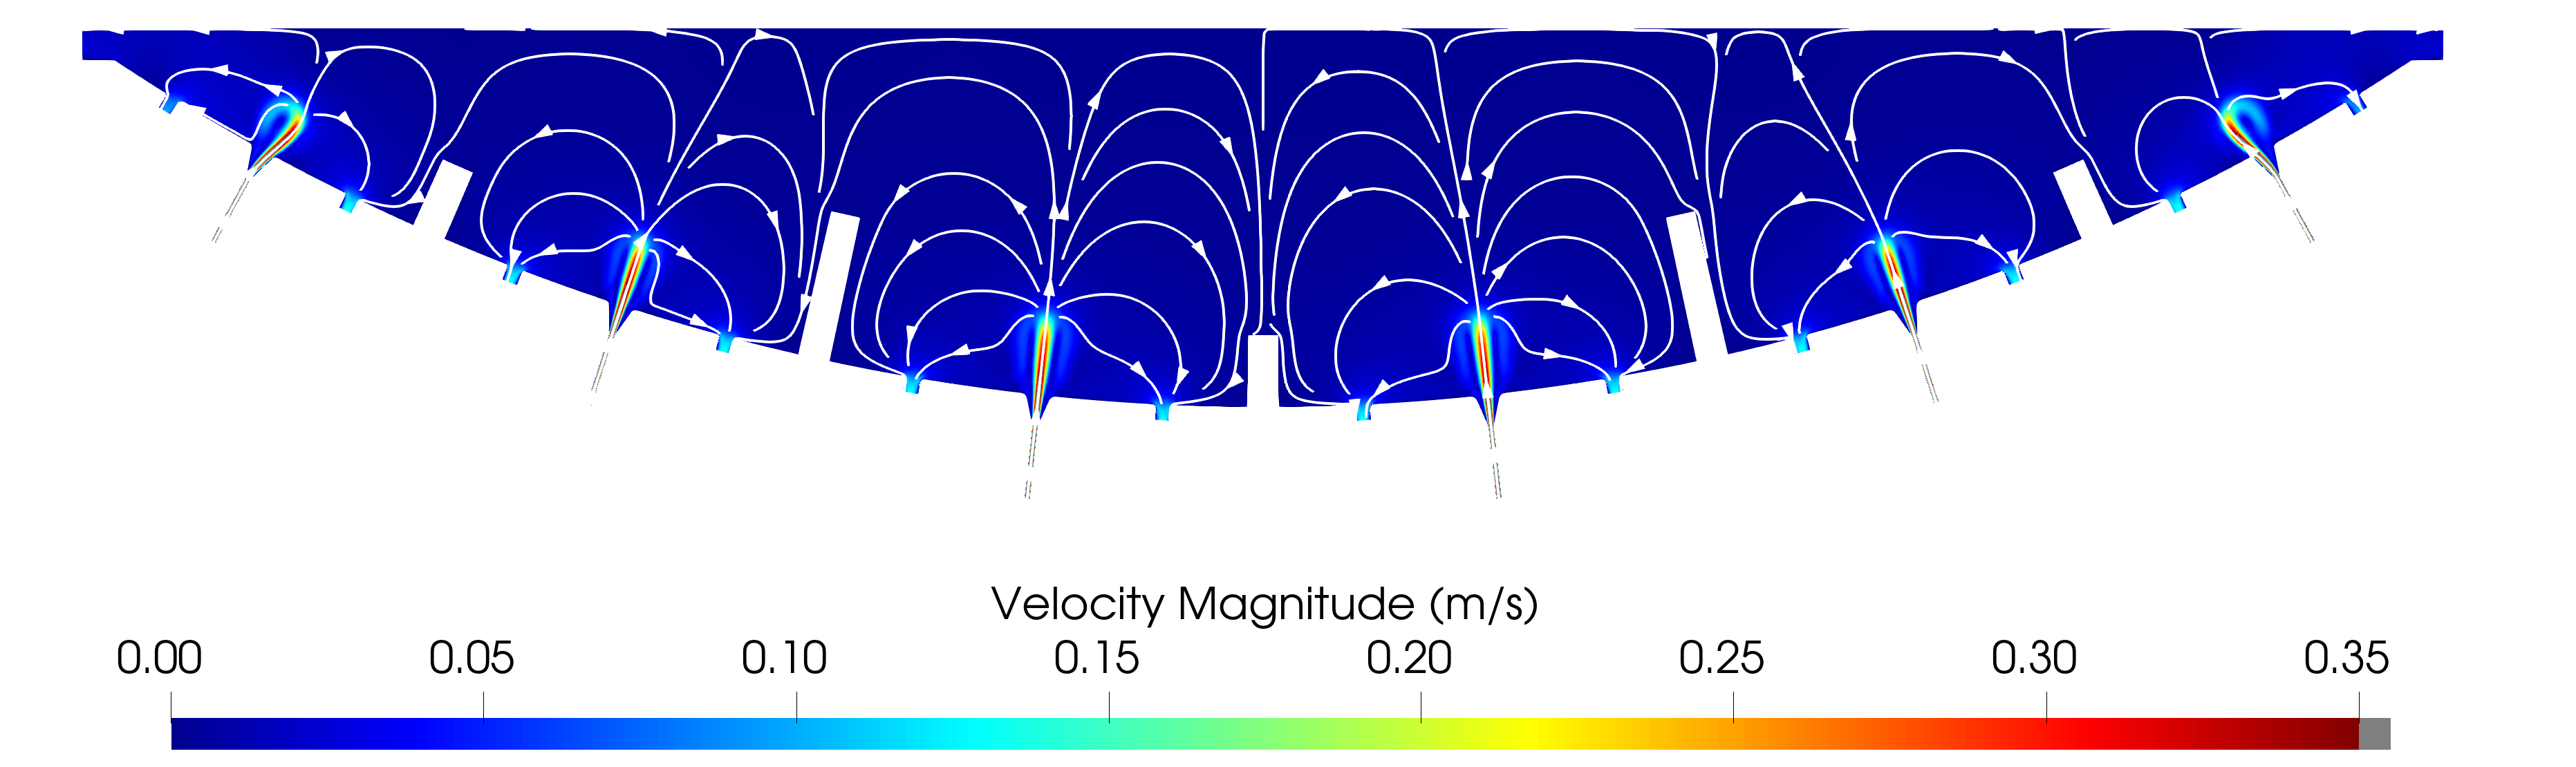
\includegraphics[width=\textwidth]{diagrams/results-variations/bifurcation-452.png}
                    \caption{}
                    \label{fig:bifurcations:452}
                \end{subfigure}
                \vfill
                \begin{subfigure}{\textwidth}
                    \centering
                    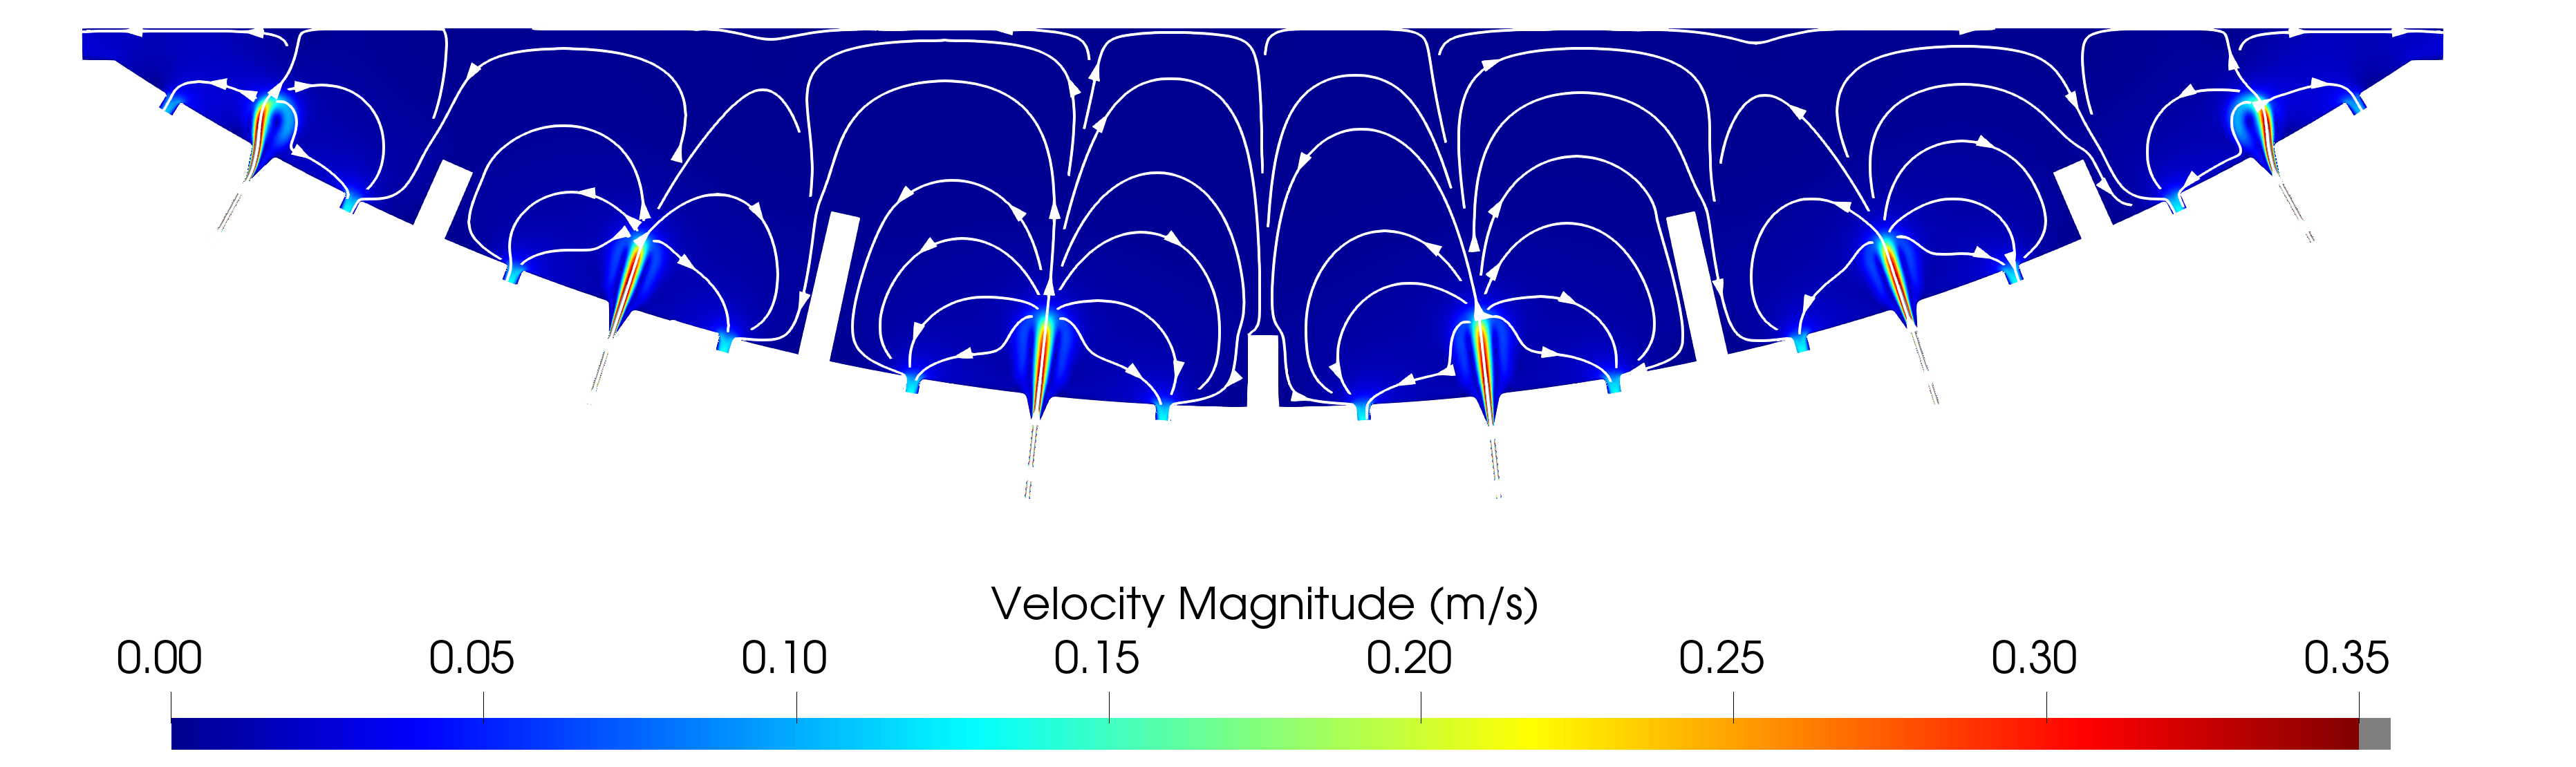
\includegraphics[width=\textwidth]{diagrams/results-variations/bifurcation-512.png}
                    \caption{}
                    \label{fig:bifurcations:512}
                \end{subfigure}
                \begin{subfigure}{0.45\textwidth}
                    \centering
                    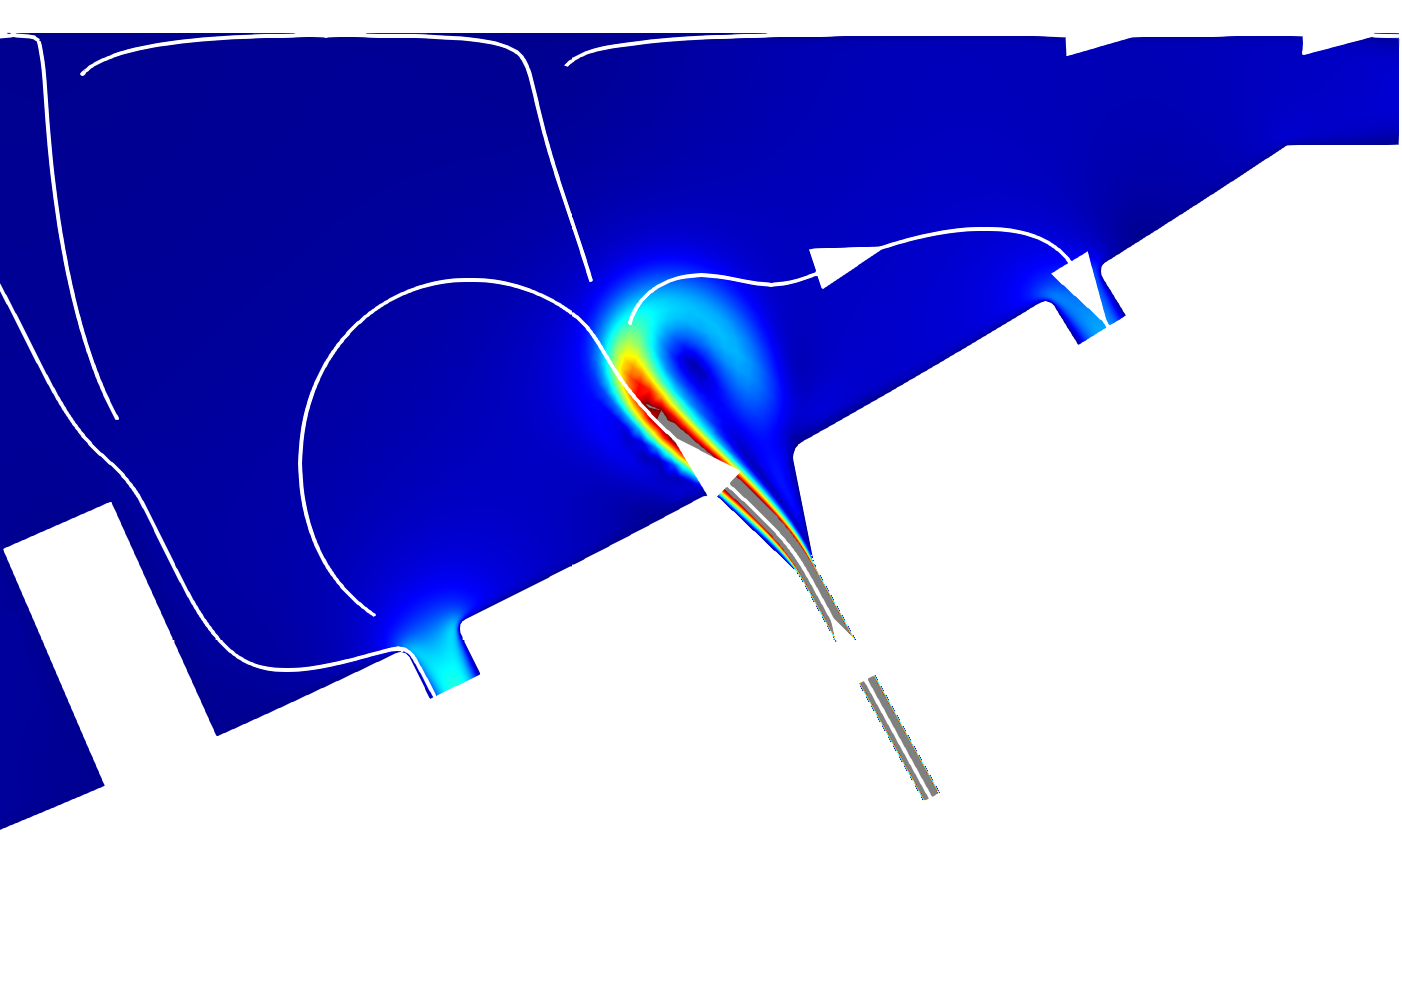
\includegraphics[width=\textwidth]{diagrams/results-variations/bifurcation-452-zoom.png}
                    \caption{}
                    \label{fig:bifurcations:452-zoom}
                \end{subfigure}
                \hfill
                \begin{subfigure}{0.45\textwidth}
                    \centering
                    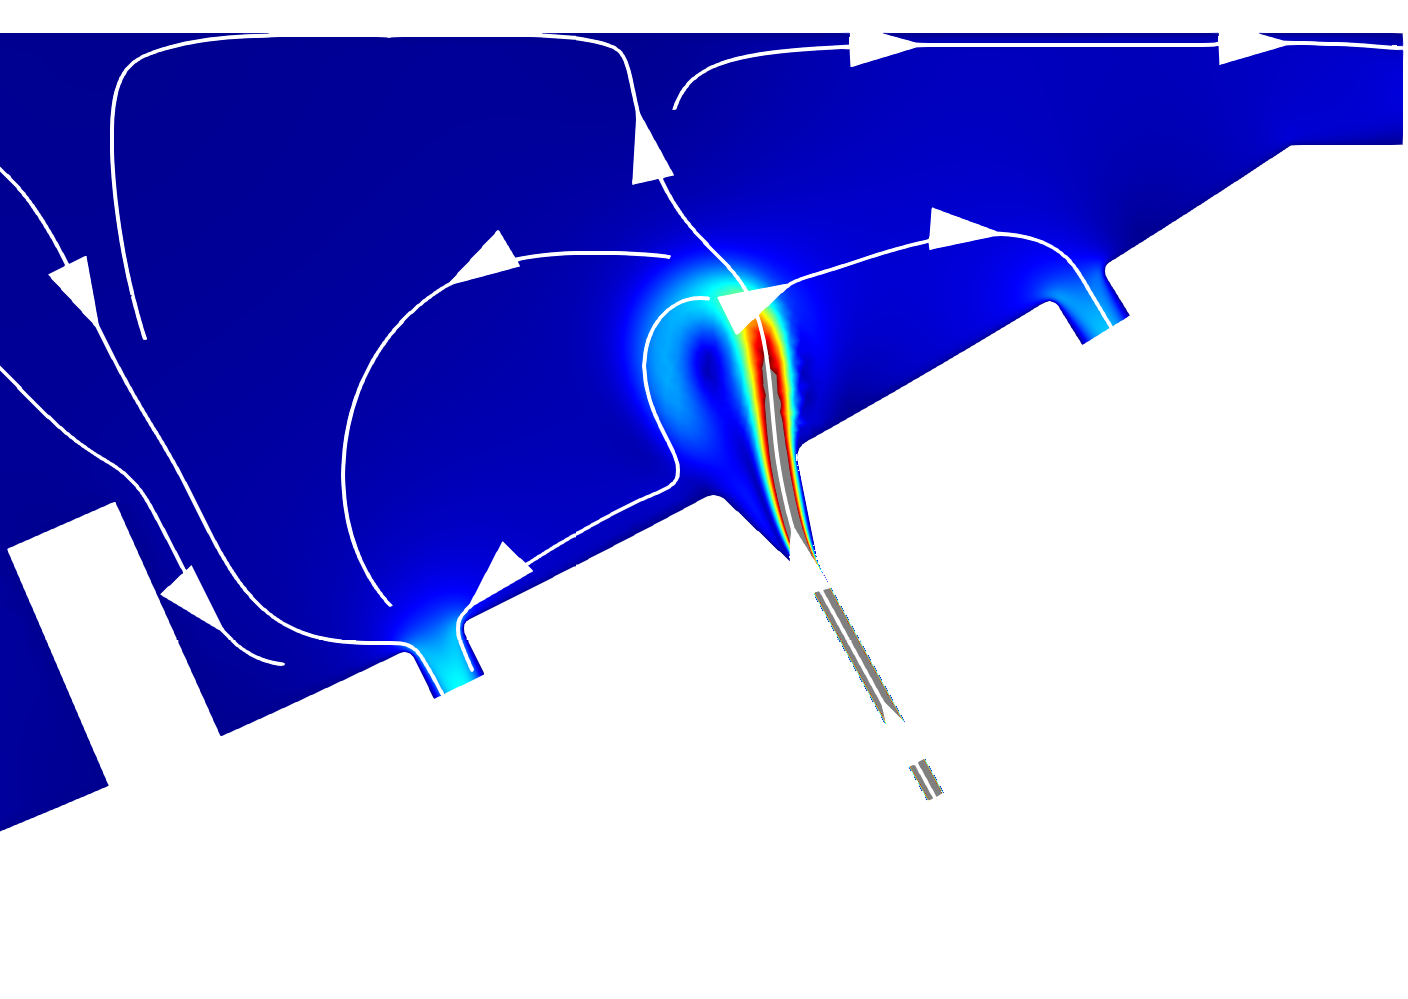
\includegraphics[width=\textwidth]{diagrams/results-variations/bifurcation-512-zoom.png}
                    \caption{}
                    \label{fig:bifurcations:512-zoom}
                \end{subfigure}

                \caption{Velocity plot with a \textit{linear} velocity magnitude colour scaling for simulations with (a) $U = \qty{0.8866}{\metre\per\second}$, and (b) $ U = \qty{0.8850}{\metre\per\second}$. (c) and (d) respectively show zoomed in views of the right-most placentones shown in (a) and (b).}
                \label{fig:bifurcations}
            \end{figure}

            Apart from the variations in number and location of vessels, this section has found that variations in $k$ and $U$ have the greatest impact on the efficiency measures.

    \section{Summary} \label{sec:nutrient-uptake:summary}  
        % Intro of what we did.
        Throughout Chapter \ref{sec:nutrient-uptake}, we have investigated the effects of various structural variations on placental function, as measured by seven chosen measures of placental efficiency. The value of the computational approach taken in this thesis is realised here, as this allowed us to explore these variations comprehensively across a large ensemble of realisations. \S\ref{sec:nutrient-uptake:variation-of-vessels} focussed specifically on variations in the number and positions of vessels, where numbers and positions of vessels were varied uniformly-at-random over $1000$ realisations, and \S\ref{sec:nutrient-uptake:variation-of-other-parameters} independently varied seven other parameters over $7000$ realisations.

        % Background and overall relevance.
        Existing work on the positioning of basal plate veins has been conducted by \citeauthor{chernyavskyMathematicalModelIntervillous2010} \cite{chernyavskyMathematicalModelIntervillous2010}, but this was restricted to a placentone with two symmetrically-placed basal plate veins. Others, such as \citeauthor{meklerImpactTissuePorosity2022} \cite{meklerImpactTissuePorosity2022} investigated the effects of many basal plate veins and their symmetry, but these were again limited to a single placentone and assumed the spiral artery was placed centrally. This thesis has considered a physically-relevant 2D placenta geometry for the first time, and has therefore allowed for a more physiologically relevant study of the influence of structural parameters than previous studies. Our results found the same `short-circuiting' behaviour reported by these previous studies, where blood exits through nearby veins and overall lowers oxygen uptake \cite{chernyavskyMathematicalModelIntervillous2010,meklerImpactTissuePorosity2022}. Whilst the results of this thesis are restricted to 2D, the computational demand is much lower than an equivalent 3D study.

        % Variability of results.
        In general, the results presented in \S\ref{sec:nutrient-uptake:variation-of-vessels} showed high variability in the values of the efficiency measures outside the interquartile range when comparing these against the varying numbers of arteries and veins, but showed a much lower variability when compared against the ratio of veins-to-arteries; this suggests that the ratio may be more important in determining flow and transport behaviour. Three of the seven parameters varied in \S\ref{sec:nutrient-uptake:variation-of-other-parameters} had very little effect on the seven placental efficiency measures; these were variations in the artery mouth width, septal wall height, and oxygen diffusivity. This was surprising in the case of the artery width, given that studies have suggested that small artery widths are related to diseased placentas, where flow enters the placenta at an order of magnitude faster \cite{burtonRheologicalPhysiologicalConsequences2009}; however, we note that the mechanism through which placental function is decreased could be due to damage to villous tree structure from the high-speed flow, rather than the behaviour that the small artery width directly influences. The other four choices of parameters --- namely vein width, oxygen uptake rate, permeability of the villous tree, and inlet blood flow speed --- had much more of an influence on our efficiency measures.

        % Slower flow and short-circuiting.
        We found that when there was a large number of veins, the flow was on average slower, due to the flow short-circuiting and exiting through nearby veins; this mirrors behaviour presented by \citeauthor{chernyavskyMathematicalModelIntervillous2010} \cite{chernyavskyMathematicalModelIntervillous2010} and \citeauthor{meklerImpactTissuePorosity2022} \cite{meklerImpactTissuePorosity2022}. \citeauthor{dellschaftHaemodynamicsHumanPlacenta2020} reported that diseased placentas generally had much less slow-moving blood, which from our results suggests that placentas with either a small number of arteries or large number of veins could be characteristic of disease. The fraction of slow flow in our simulations was two times lower than that reported in vivo by \citeauthor{dellschaftHaemodynamicsHumanPlacenta2020} \cite{dellschaftHaemodynamicsHumanPlacenta2020}, which could be due to the relatively large number of vessels to domain size in the 2D flow presented here, and highlights one of the restrictions of our 2D study.

        % Oxygen.
        We found that the number of arteries, the IVS permeability, the inlet blood flow speed, and (unsurprisingly) the oxygen uptake rate had the biggest influence on oxygen uptake. For the variations in the number of arteries, we found that the uptake rate is most affected due to each artery introducing a higher flux of flow and oxygen. For the variations in permeability, we instead found that higher speed flow penetrated deeper into the placenta, allowing a larger surface area for oxygen uptake. The results of \citeauthor{serovOptimalVilliDensity2015} \cite{serovOptimalVilliDensity2015} found an optimal density of the villous tree to enable the highest oxygen uptake, which balances resistive flow and uptake effects. However, our results found no such optimal value, instead finding that a more permeable villous tree gave the highest uptake. A reason for this is, unlike \citeauthor{serovOptimalVilliDensity2015} \cite{serovOptimalVilliDensity2015}, we did not simultaneously investigate changes to the uptake rate due to increased villous surface area, which is likely the driver of an optimal villous density. Additionally, we found that higher inlet blood flow speeds decreased oxygen uptake, which supports the work of \citeauthor{burtonRheologicalPhysiologicalConsequences2009} \cite{burtonRheologicalPhysiologicalConsequences2009}.

        % Venous drainage.
        We also studied venous drainage routes, finding that flow had a slight preference for septal wall veins over basal plate veins for all choices of number of vessels; however, we remarked that this could simply be due to the higher number of septal wall veins available for exit ($15$ septal wall veins, as opposed to $12$ basal plate veins). Interestingly, we found oxygen leaving the placenta at a high concentration (approximately $85\%$ of what entered) in almost all the variation studies. This is oxygen that could have been uptaken by the villous tree to be delivered to the fetus, but instead exits the placenta and returns to the maternal circulation.

        % Limitations of the measures themselves.
        The approach of this chapter was to consider several thousand realisations of flow and oxygen concentration fields. On this scale, we cannot make useful comparisons by visualising every individual flow and oxygen transport field, and therefore we turned to seven lower-dimensional measures, where each measure was chosen such that the main features of the fields are captured. However, there are several other choices of measure that would have given us further insight into flow and oxygen transport behaviour. For example, measures characterising vessel position or outlet routes via particle tracking would likely have been of value in this chapter's analysis, as these are features that our measures do not capture and are likely important to blood flow and oxygen transport. Furthermore, studies of the heart have used energy measures that incorporate the fluid pressure (e.g., \cite{rijnbergEnergeticsBloodFlow2018,whiteheadNonlinearPowerLoss2007}), which likely would have been relevant to our study of variations involving the villous tree.

        % Vein limitations.
        Three venous drainage aspects we did not investigate were (i) the position of veins, (ii) the relative importance of septal wall veins and basal plate veins, and (iii) the impact of removal of marginal sinuses. Therefore, an interesting piece of future work could be to either vary the number of septal wall veins separately from basal plate veins (so that we understand their sole influence), or to study the effect of septal wall vein position more carefully; for example, the green- and red-boxed simulations from Figure \ref{fig:mega-vessels1:simulations} appear to show a large flux of blood being drawn to septal wall veins that occur higher up on the septal walls. A further simplification during \S\ref{sec:nutrient-uptake:variation-of-vessels} is that we varied the position of the vessels simultaneously to the number of vessels; an obvious next step would be to consider these effects separately.

        % Limitations on vessel placement for second part.
        The number and position of vessels are an assumption that may affect results, especially in \S\ref{sec:nutrient-uptake:variation-of-other-parameters} where vessels were placed symmetrically. For simplicity, we parameterised our 2D placenta geometry such that there were at most one artery per placentone, two basal plate veins per placentone, three septal wall veins per septal wall, and two permanently retained larger marginal sinus veins; in reality, there may be no such restrictions, and could have an effect on the results presented here.

        % Limitations with comparisons to data.
        We compared some of our results to previous experimental data of mean placenta speed and slow flow percentage. Overall, we found that our simulated flow speeds were faster than what is reported in the literature, and that our slow flow percentage was roughly twice as small as what is reported by \citeauthor{dellschaftHaemodynamicsHumanPlacenta2020} \cite{dellschaftHaemodynamicsHumanPlacenta2020}. This disparity could be due to the 2D study of flow in this thesis, or due to unphysical parameter regimes chosen for the variations.

        % Cross-flow flux (relevant to other chapters).
        A unique aspect we studied in comparison to other studies is the flux of blood passing between placentones, which other studies have necessarily neglected due to considering only placentone geometries. We found that the amount of blood passing over septal walls (termed `cross-flow flux' here) on average had a non-monotonic relationship with the number of arteries. Our results indicated that there needs to be a careful balance between more arteries driving an overall larger volume of blood, and asymmetric placement of arteries to encourage flow to exit through non-adjacent veins. However, we did also find that there was a much larger variation in cross-flow flux for varying numbers of arteries, likely due to effects from the number of veins. Variations in the number of veins were much more impactful, giving much higher cross-flow flux for lower numbers of veins; higher numbers of veins likely created opportunities for entering arterial flow to short-circuit and easily exit through nearby veins. Study of the cross-flow flux for varying inlet blood flow speed highlighted an interesting bifurcation phenomenon, where the jets of blood entering the peripheral placentones would prefer either the left or right side of the central cavity, even when the values of $U$ were relatively similar. Bifurcations of the steady 2D Navier-Stokes equations have been documented by \citeauthor{cliffeAdaptivityPosterioriError2012} \cite{cliffeAdaptivityPosterioriError2012}, where they obtained a critical Reynolds number at which a bifurcation occurs of $\Re \approx 40.6$ in the context of a widening channel domain that expands with a 3-to-1 ratio; whilst the widening spiral artery of the placenta and widening channel domains are different, the Reynolds number at the base of the spiral artery mouth in our aforementioned simulations was $\Re \approx 110$, so it is reasonable that these phenomena are related.

        % Key findings + oxygen uptake and disease.
        One key observation of this chapter is that, of the parameter variations we have considered in this chapter, variations in the number of vessels are the most impactful on flow and oxygen concentration behaviour. Additionally, oxygen uptake is arguably the most important function of the placenta that we consider here; overall, our results found that low numbers of arteries, high numbers of veins, low permeability of the villous tree, and high-speed inlet blood flow reduce oxygen uptake, which may be characteristic of placental diseases such as PE and FGR.

        % Next chapter.
        The following chapter will take this thesis in a different direction to this chapter, instead investigating how we may compute numerical MRI signals from a computed velocity field. This allows us to directly compare MRI signals from real-world placentas with our computed MRI signals of our simulations of maternal blood flow.

        % LOOSE SENTENCES
        % Interestingly, as the first and third columns of Figure \ref{fig:mega-other} show that almost all the efficiency measures change very little due to varying the artery width and wall height. The only exception is that there is a slightly higher total energy, $E_\text{total}$, for small artery widths. \citeauthor{burtonRheologicalPhysiologicalConsequences2009} \cite{burtonRheologicalPhysiologicalConsequences2009} reported that PE placentas are characterised by non-widening arteries such as these, which ultimately leads to faster blood entering the placenta that damages the villous tree and leads to shorter circulation times. Our model does not show this, but this disparity could be due to not capturing villous structure damage in our modelling.
        
        % The remainder of \S\ref{sec:nutrient-uptake:variation-of-other-parameters} will consider variations to permeability, $k$. In varying $k$, we note that we are actually changing the value of the \textit{maximum} permeability, as we retain the smooth transition behaviour described in Equation \eqref{eq:smooth-transition}. We note that the nominal value of $k$ from Table \ref{tab:structural-parameters} is \qty{1e-8}{\metre^2}. 

        % We remark that the values of $v_\text{cross}$ are in general lower here, due to the geometry here containing symmetric placement of arteries and veins.

        % \todoitemone{George's data says: 57\% is slow and 6\% is fast.}

        % \todoitemone{Lots of loose sentences...}
        % the number of veins has a much stronger influence on flow and oxygen transport behaviour than the number of arteries. We also noted that, in general, much faster flow was presented here than in \S\ref{sec:numerical-methods:blood-flow-experiments}; this is due to flow in \S\ref{sec:numerical-methods:blood-flow-experiments} being symmetric.

        % Taking a different approach, \S\ref{sec:nutrient-uptake:variation-of-other-parameters} instead kept the symmetric placement of basal plate vessels that was originally presented in \S\ref{sec:numerical-methods:blood-flow-experiments}, and separately varied three parameters from Table \ref{tab:structural-parameters}. This is related to work by \citeauthor{serovOptimalVilliDensity2015} \cite{serovOptimalVilliDensity2015}, where they performed many simulations over cylinders (used to represent villi), and were able to find an optimal villi density in order to maximise oxygen uptake. Our results indicated that septal wall heights and artery width have very little influence on our chosen efficiency measures; however, other authors have predicted that small artery widths --- which are generally associated with diseased PE and FGR placentas --- should negatively impact oxygen uptake. We noted that this disparity could be due to damaged villous tree structures, the effects of which are not captured in our modelling.

        % There are a number of limitations to our approach here. Firstly, we considered a lot of these variations in isolation to each other, which likely masks some possible interacting behaviour. Secondly, there is uncertainty is several of the other parameters in Tables \ref{tab:structural-parameters} and \ref{tab:problem-parameters} which we have not considered; these include varying the vein width (including independently varying the vessel widths), varying central cavity size (cf. \cite{chernyavskyMathematicalModelIntervillous2010}), and the oxygen diffusivity or uptake rate; no definitive conclusions can be deduced from a study that does not consider all sources of possible error. Thirdly, we made some strong assumptions on the ordering of vessels on the basal plate, as well as the number of vessels allowed to exist on the basal plate and septal walls, which of course would ideally be relaxed.

        % \todoitemtwo{Cite others that did other nutrients other than oxygen.}